\section*{Introduction}\index{Acercaria}
Here we begin looking at taxa classified in \textbf{Acercaria}, a taxon characterized in part by the presence of stylate laciniae. These three orders, Hemiptera, Psocodea, and Thysanoptera, may comprise a monophyletic lineage that is sister to Holometabola (the taxon with truly larval immature stages). Alternatively, based on genome-scale molecular data \citep{Misof763}, these taxa are related as ((Thysanoptera, Hemiptera),(Psocodea, Holometabola)). Acercaria share the following characteristics \citep{beutel2013insect}; do they represent synapomorphies?

\begin{itemize}
\item legs with $\le$3 tarsomeres
\item cerci absent 
\item labial palps relatively small or absent 
\item maxilla modified into stylet (maxillary laciniae are separated from the rest of the maxilla and are stylet-like)
\item postclypeus relatively large, accommodates cibarial dilator muscles for sucking
\item many species with inactive stage prior to adult
\end{itemize}

\section{Hemiptera (true bugs, scale, aphids, hoppers, \textit{etc}.)}\index{Hemiptera}
\noindent{}\textit{Diagnostic characters:} antenna usually with 5--10 antennomeres, sometimes reduced; piercing/sucking mouthpart (mandible and maxillae rod-like stylets); labium elongate, multi-segmented and surrounds the stylets posteriorly (beak); prothorax is usually wider than long; fore wing is sometimes more sclerotized than hind wing (\textit{e.g.}, Heteroptera); arolium (apicomedial membraneous area of pretarsus) balloon shaped, often exceeds tarsal claw apically, sometimes absent, not eversible; cercus absent.\vspace{3mm}

\subsection{Sternorrhyncha (psyllids, whiteflies, aphids, scale insects)}\index{Sternorrhyncha}
\noindent{}\textit{Diagnostic characters:} tarsi 1- or 2-segmented; antennae filiform, sometimes absent labium arises from the head in between the procoxae when the head is in normal position, sometimes reduced; ovipositor reduced.\vspace{3mm}

\subsubsection{Psylloidea (plantlice)}\index{Psylloidea}
\noindent{}\textit{Diagnostic characters:} tarsi 2-segmented; antennae usually with 10 antennomeres; fore wings often more sclerotized than hind wing; superficially resemble tiny cicadas.\vspace{3mm}

\noindent{}\textit{Natural history:} More than 800 species of plantlice have been described worldwide, and several species are important pests (\textit{e.g}., \textit{Diaphorina citri} Kuwayama, 1908 and \textit{Trioza erytreae} Del Guercio, 1918, which both vector the bacterium that causes citrus greening).\vspace{3mm}

\begin{figure}[ht!]
 \centering
 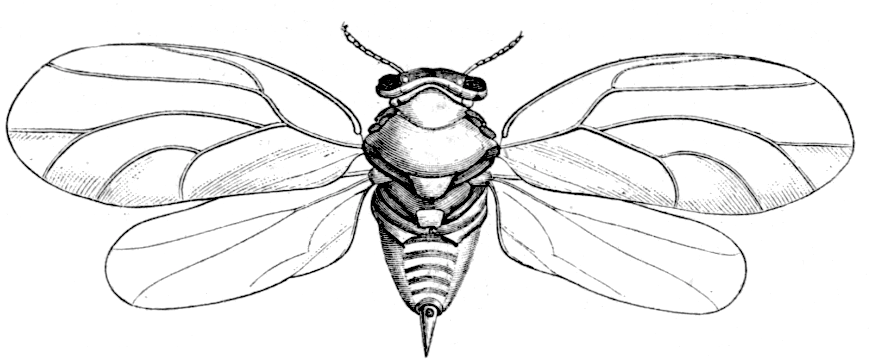
\includegraphics[width=0.6\textwidth]{acercaria/PsyllidHabitus}
 \caption{Psylloidea habitus \citep[][Fig. 10d]{bhlpart17516}}
 \label{fig:psyllid}
\end{figure}

\subsubsection{Aleyrodidae (whiteflies)}\index{Aleyrodidae}
\noindent{}\textit{Diagnostic characters:} tarsi 2-segmented, antennae 7-segmented (figure \ref{fig:aleyrodid1}); hind wing almost as large as fore wings; wings held horizontally over body while at rest; body and wings covered with white, waxy powder (depending on preservation) (figure \ref{fig:aleyrodid2}).\vspace{3mm}

\noindent{}\textit{Natural history:} More than 1,500 species are known worldwide, including many pest species. The typical whitefly life cycle is, at least superficially, similar to holometabolous development. Immature stages are even referred to as larvae, and the resting stage prior to eclosion of the adult is called the pupa or puparium (the resting stage resides inside the cast skin of an earlier instar).\vspace{3mm}

\begin{theo}
{}What is the function of the white ``powder'' that covers whitefly bodies? How would you test your hypothesis?
\end{theo} 

\begin{figure}[ht!]
 \centering
 \begin{subfigure}[ht!]{0.12\textwidth}
  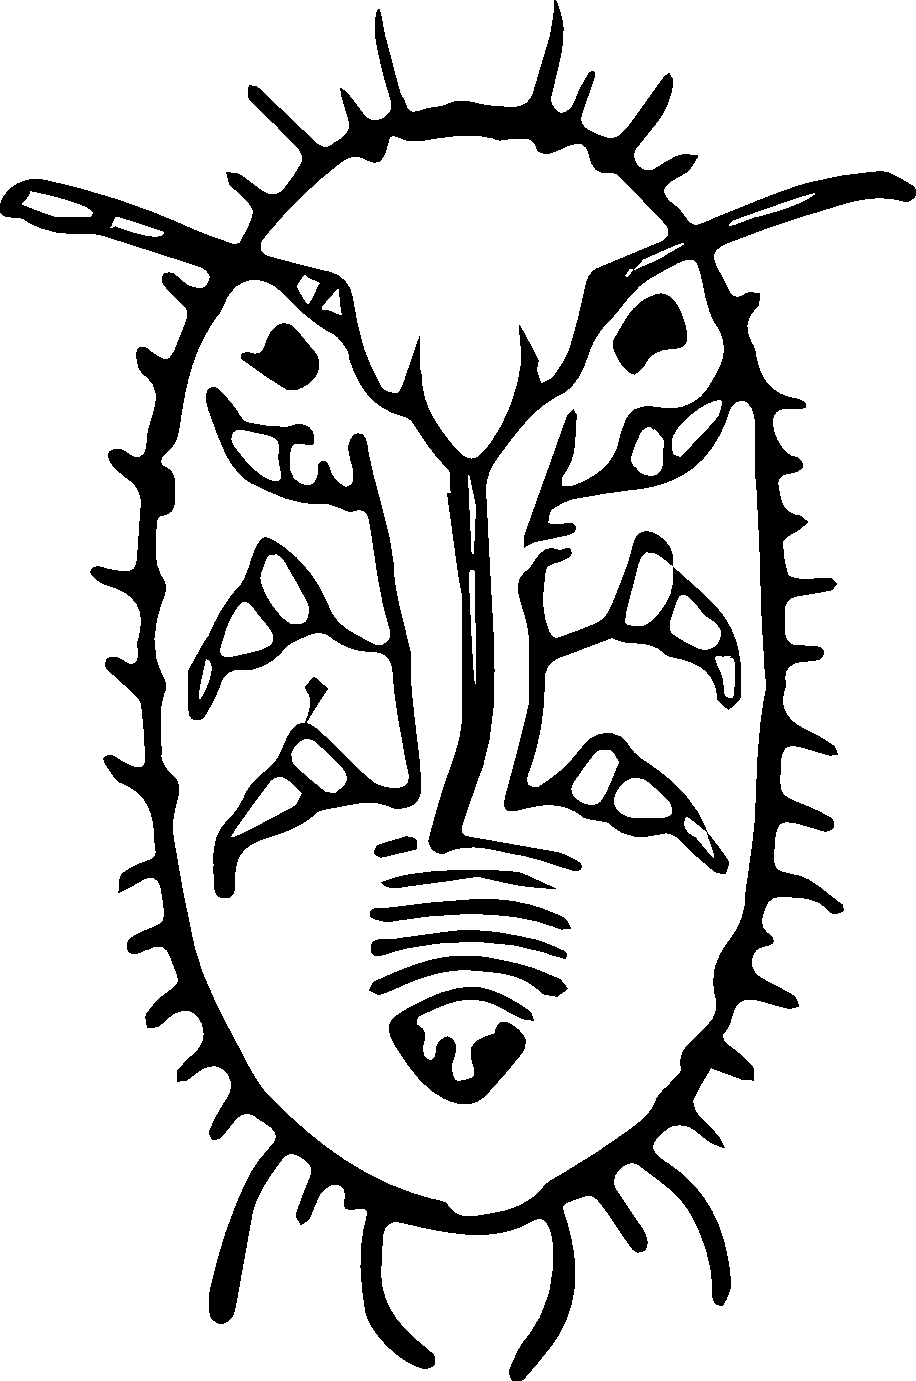
\includegraphics[width=\textwidth]{acercaria/aleyrodid1}
  \caption{}
  \label{fig:aleyrodid1}
 \end{subfigure}
 \hfill
 \begin{subfigure}[ht!]{0.3\textwidth}
  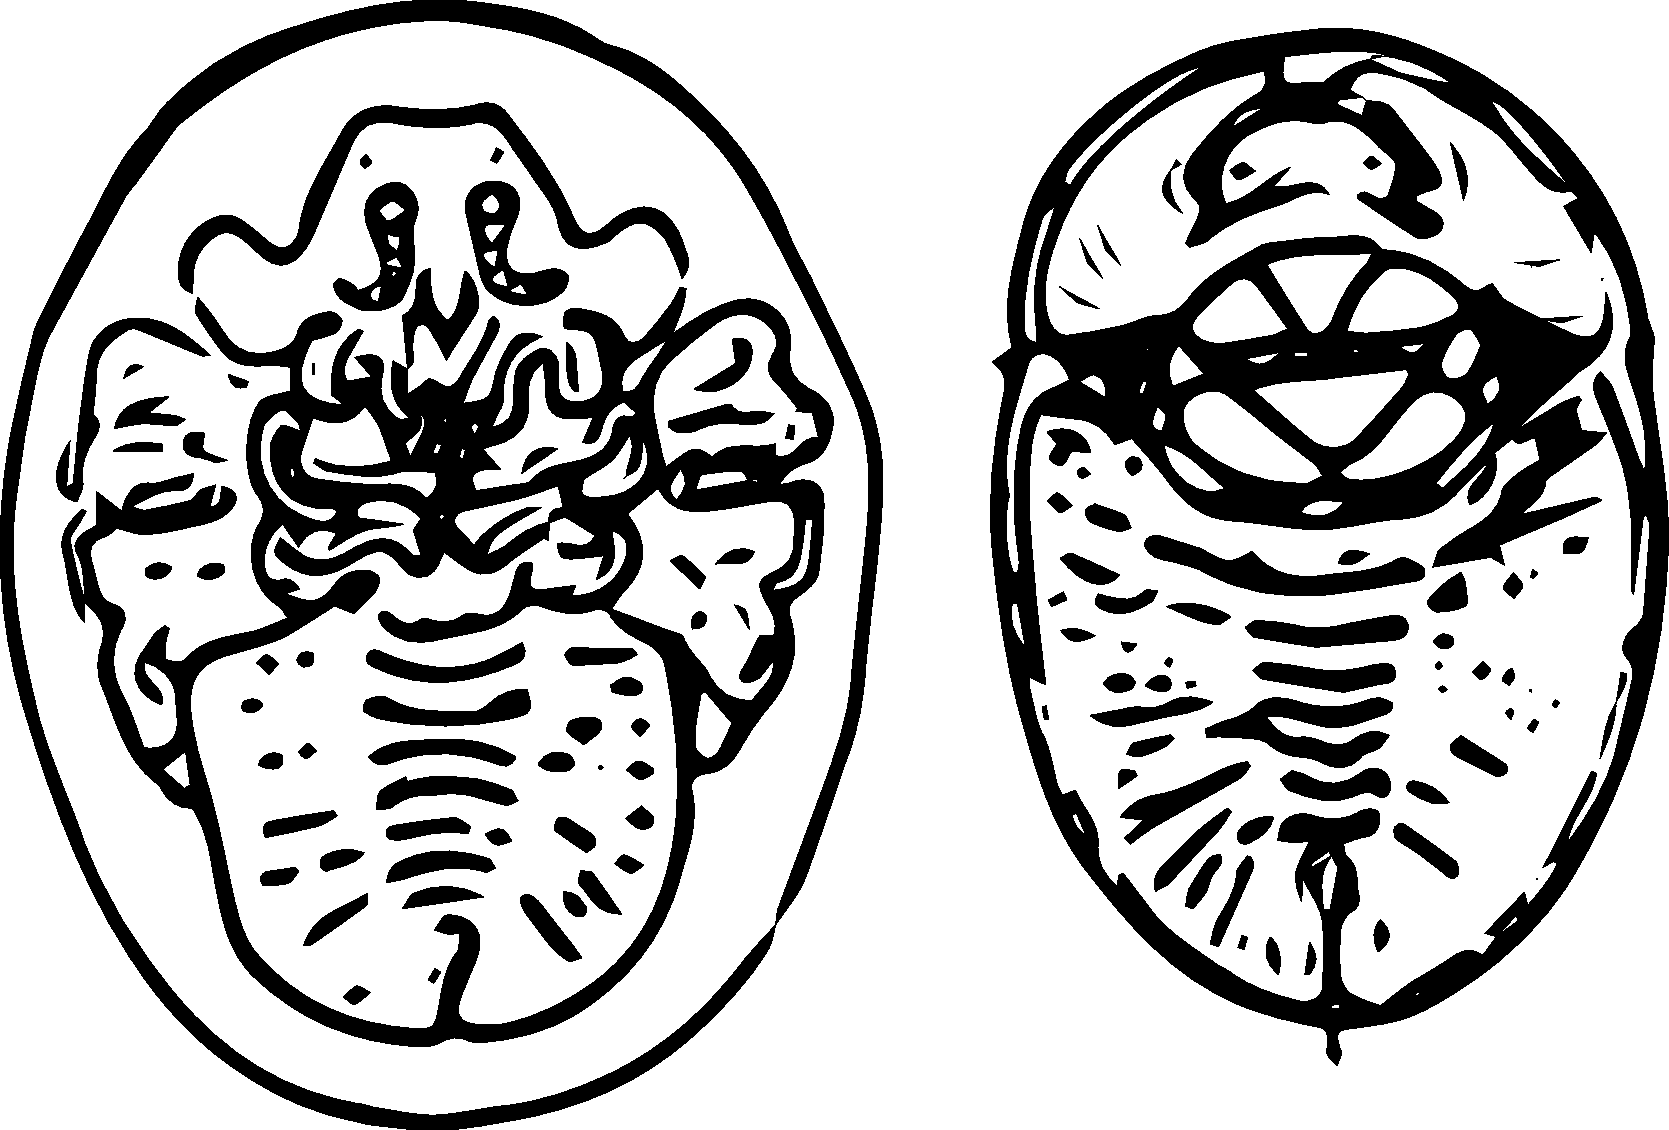
\includegraphics[width=\textwidth]{acercaria/aleyrodid2}
  \caption{}
  \label{fig:aleyrodid2}
 \end{subfigure}
 \hfill
 \begin{subfigure}[ht!]{0.53\textwidth}
  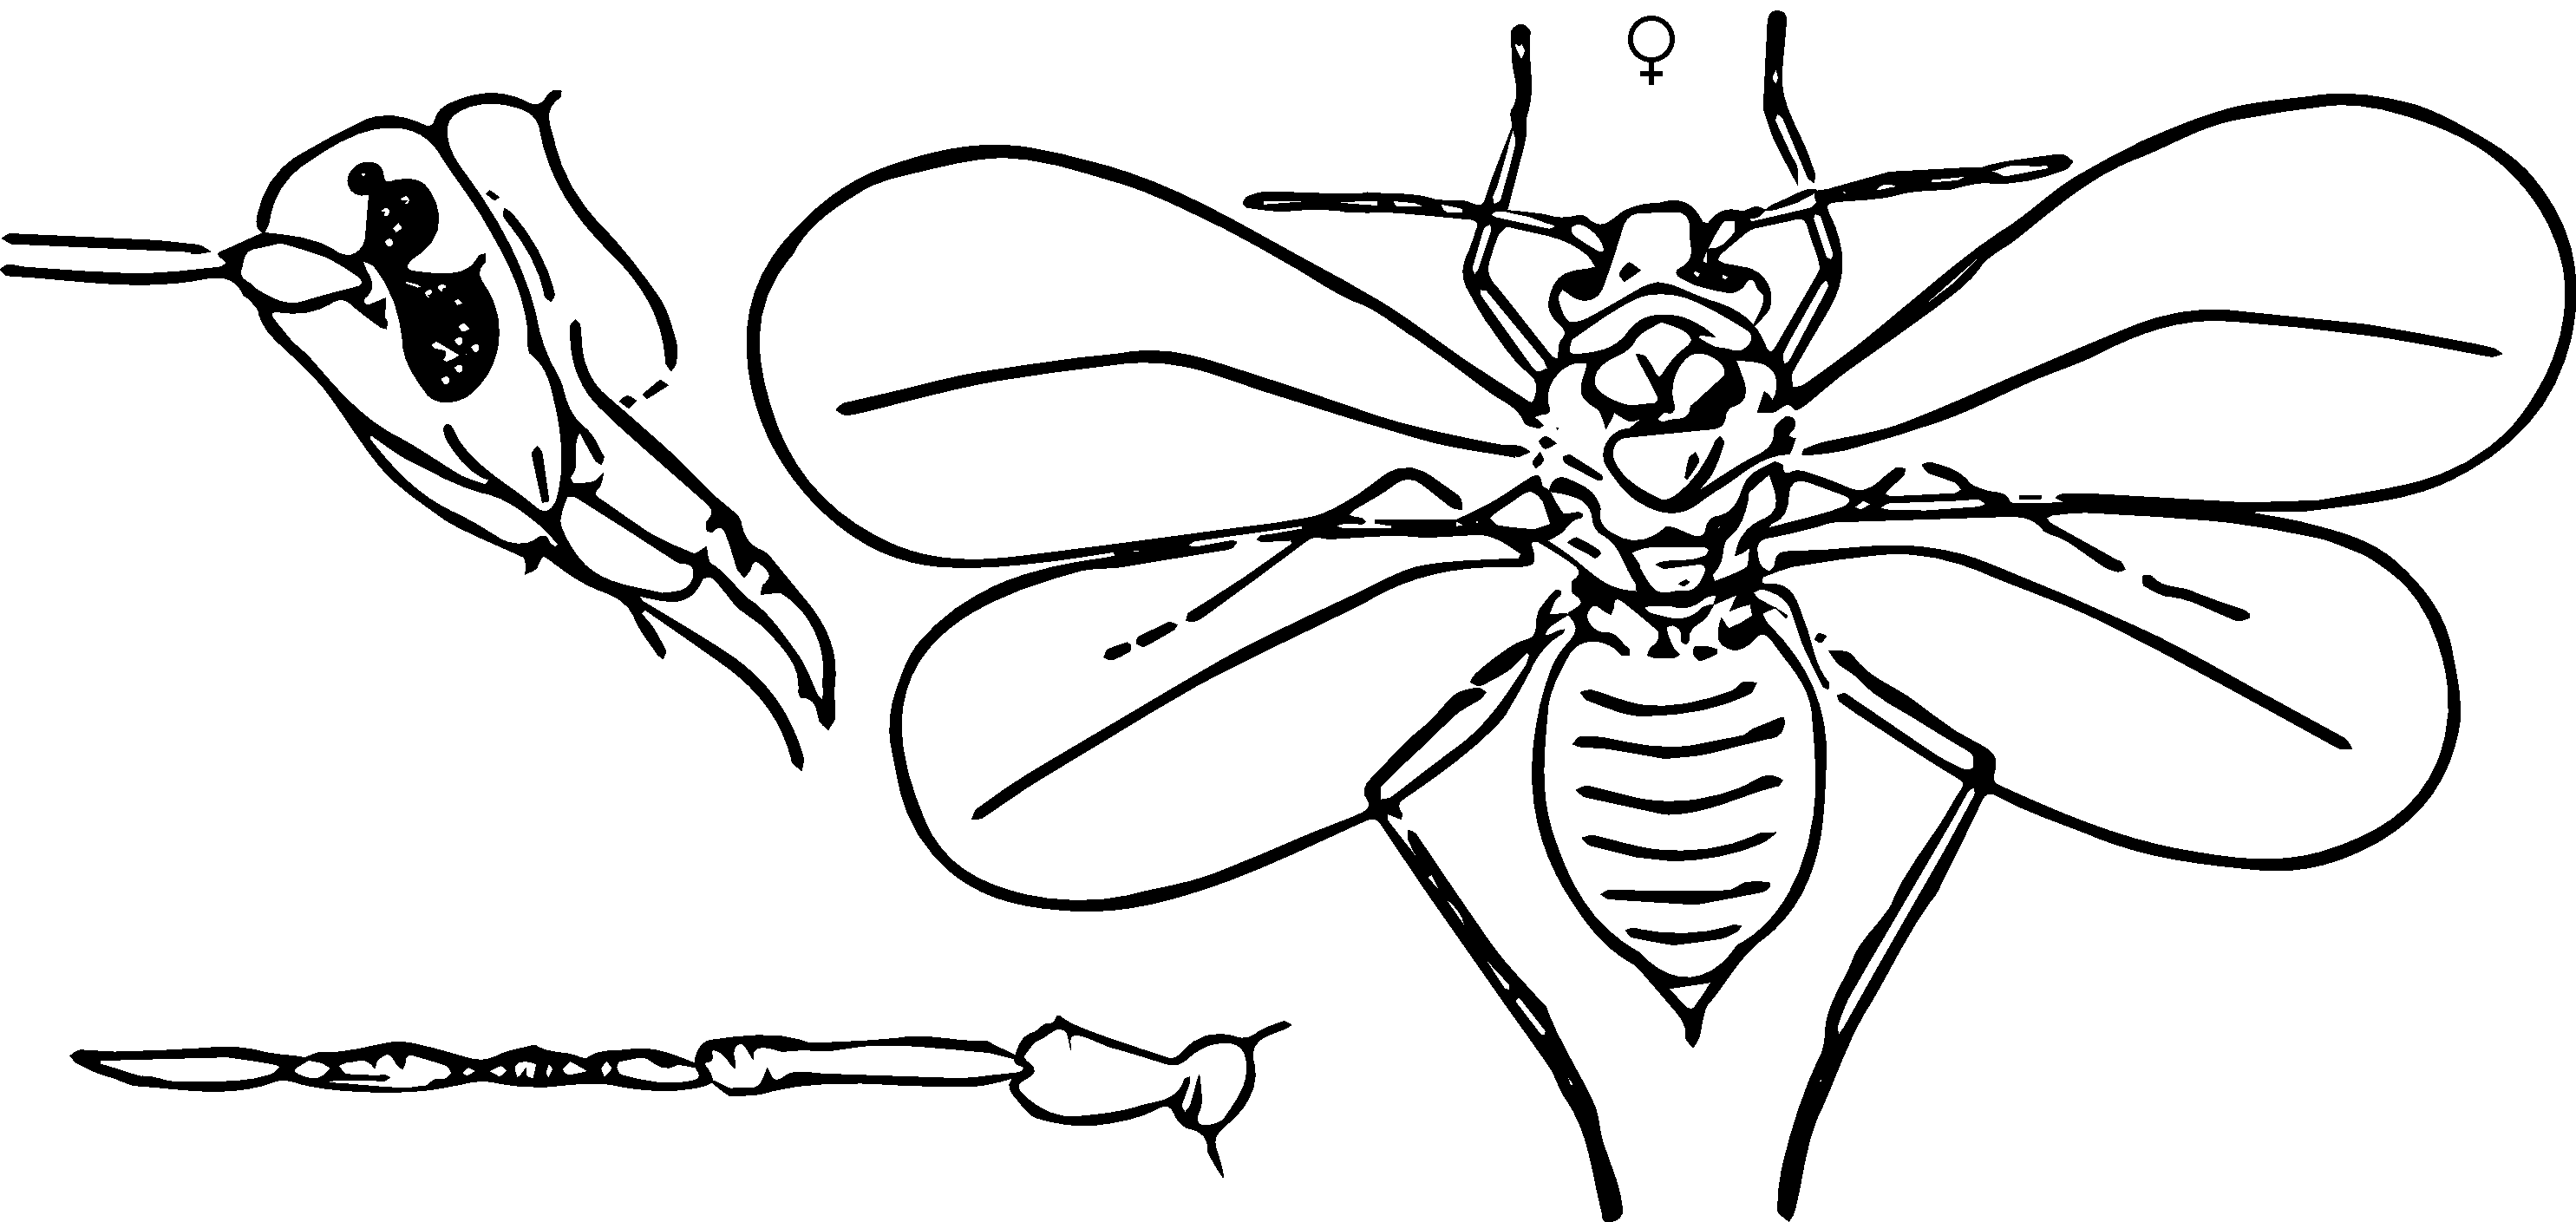
\includegraphics[width=\textwidth]{acercaria/aleyrodid3}
  \caption{}
  \label{fig:aleyrodid3}
 \end{subfigure}
 \caption{Aleyrodidae. \textbf{(a)} Nymph/larva; \textbf{(b)} pupae; \textbf{(c)} adult head, dorsal habitus, antenna \citep[][Figs. 8,9]{bhlitem192425}}\label{fig:aleyrodid}
\end{figure}

\subsubsection{Coccomorpha (scale insects, mealy bugs, \textit{etc}.)}\index{Coccomorpha}
\noindent{}The classification within this infraorder remains in flux, with possibly two superfamilies and more than 30 extant families. They share the following characteristics: adult males winged, 1-segmented tarsi (rarely 2), 1 pair of wings, no beak; females always wingless, sometimes legless or nearly so, often with a waxy or scale-like covering; first instar nymphs (``crawlers'') are quite mobile and have distinct legs and antennae.\vspace{3mm}

\noindent{}These insects also live primarily sedentary lives, with virtually no locomotion after the first instar or ``crawler'' stage (at least for females). As you examine these scale specimens, think about their adaptations to this kind of lifestyle. Spend time with both the specimens we have \textit{in situ} (\textit{i.e.}, on a branch or leaf) and the slide-mounted specimens. For the latter specimens try to find the following structures, which are important for family-level diagnostics:
\begin{itemize}
    \item proboscis
    \item antennae
    \item legs
    \item anal opening
    \item adominal spiracles (may be absent in some taxa)
\end{itemize}

\noindent{}We'll look at one family, Diaspididae, which should give you a sense of the phenotypes used in diagnosing lower-level taxa.\vspace{3mm}

\subsubsection{Diaspididae (armored scale insects)}\index{Diaspididae}
\noindent{}\textit{Diagnostic characters:} adult female flattened, disc-like with hard covering formed of wax and cast skins of earlier instars; antenna reduced to one segment; terminal abdominal segments form fused pygidium, anal opening without setae; legs absent.\vspace{3mm}

\noindent{}\textit{Natural history:} A diverse family of scale insects, with well over 2,500 described species. Exuviae from early instars, along with plant material and even frass, are often incorporated into a protective ``shell'' that can be quite tough. Like other scale families, this one includes some important pests.\vspace{3mm}

\begin{figure}[ht!]
 \centering
 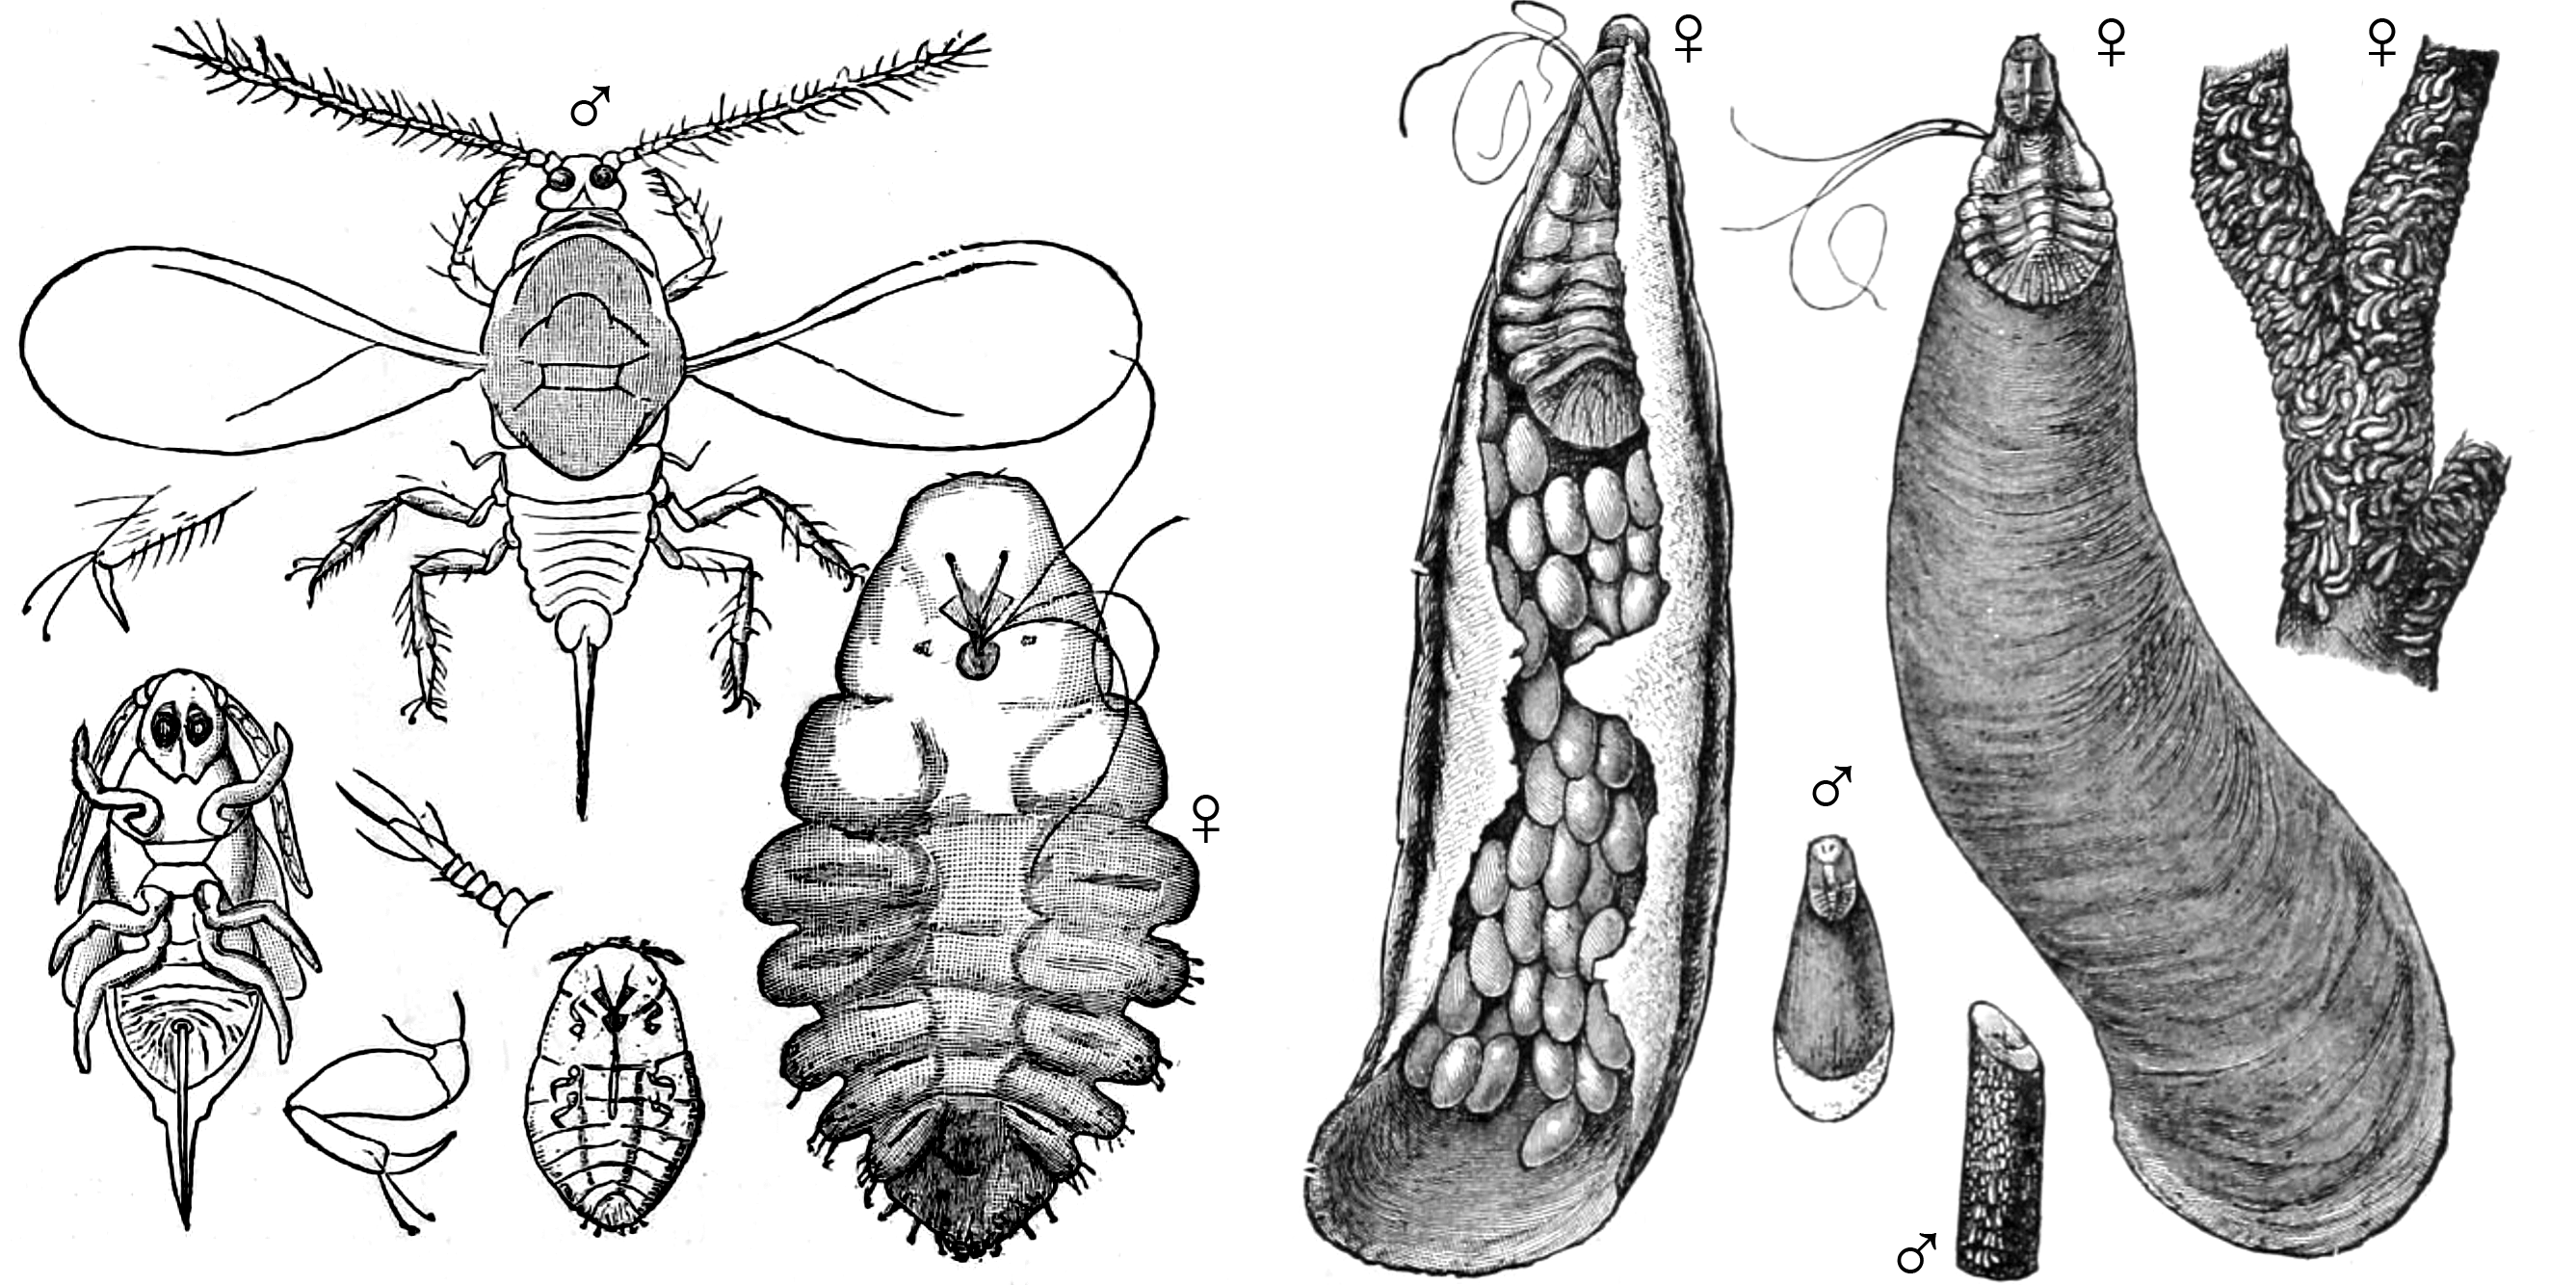
\includegraphics[width=0.85\textwidth]{acercaria/diaspidid}
 \caption{Diaspididae \citep[][Figs. 2,4]{bhlitem108079scale}}
 \label{fig:diaspidid}
\end{figure}

\begin{theo}
{}Describe three adaptions you observed in these insects that allow them to live in one location for most of their lives. What challenges does this life history present? Given these challenges why don't they have many sclerites?
\end{theo} 

\subsubsection*{Aphidomorpha (aphids, adelgids, phylloxerans)}\index{Aphidomorpha}
This taxon includes four extant families, the largest of which is Aphididae (below), and many economically and ecologically important species. 

\subsubsection{Aphididae (aphids)}\index{Aphididae}
\noindent{}\textit{Diagnostic characters:} tarsi 2-segmented, antennae usually 6-segmented; hind wing much smaller than fore wings; cornicles present near posterior end of abdomen (figure \ref{fig:aphid1}).\vspace{3mm}

\noindent{}\textit{Natural history:} More than 4,000 species have been described worldwide, and at least 250 are known to be pests if the conditions are right. Diversity is higher in the temperate zone. These species have been studied extensively in the context of ecological and symbiotic interactions. They survive primarily as phloem-feeders.\vspace{3mm}

\begin{figure}[ht!]
 \centering
 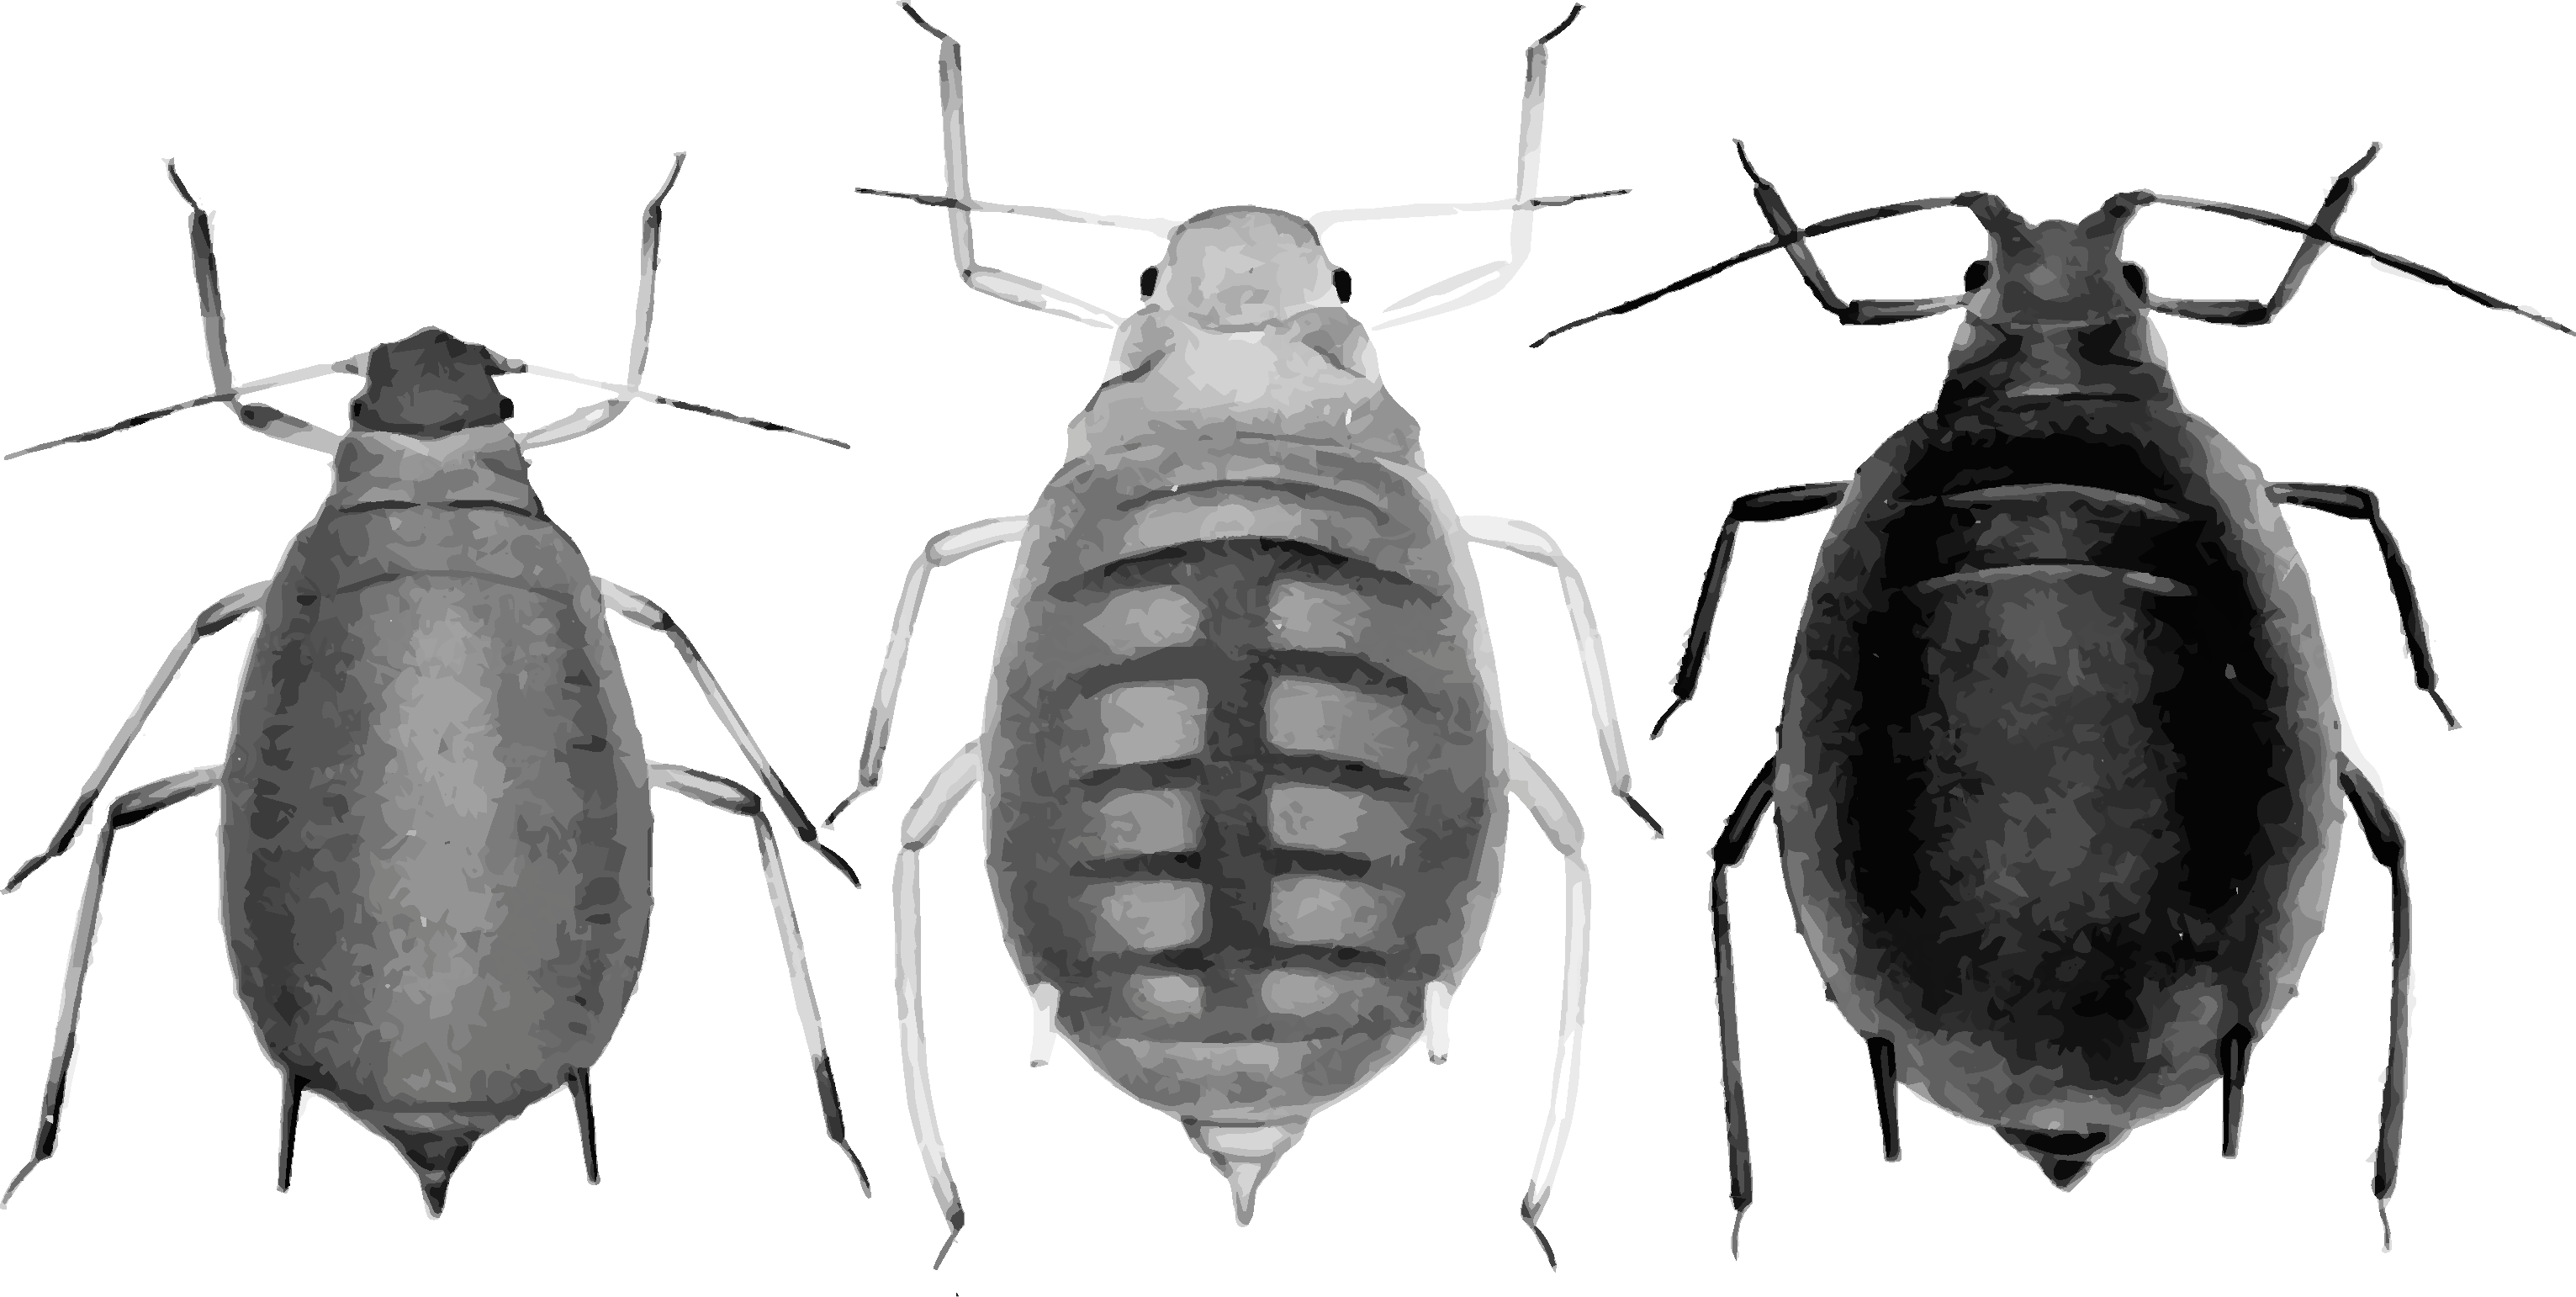
\includegraphics[width=0.6\textwidth]{acercaria/aphids}
 \caption{Aphididae habitus (S. W. Frost illustration)}
 \label{fig:aphid1}
\end{figure}

\subsection{Auchenorrhyncha (cicadas, hoppers)}\index{Auchenorrhyncha}
\noindent{}\textit{Diagnostic characters:} head hypognathous, mouthparts arises posteroventrally from head; labium arises from the head anterior to the procoxae when the head is in normal position; antennae aristate; fore wing is not more sclerotized as hind wing; tarsi 3-segmented; presence of a complex tymbal acoustic system on abdominal segment 1; ovipositor well developed.\vspace{3mm}

\subsubsection*{Cicadomorpha}

\subsubsection{Cicadidae (cicadas)}\index{Cicadidae}
\noindent{}\textit{Diagnostic characters:} relatively large (\textgreater{}2 cm); antennae arise between compound eyes that are widely separated (figure \ref{fig:cicadidae}); hind tibiae without large apical spur (\textit{i.e.}, a moveable projection); hind tibia without robust lateral and apical spines; tymbals present.\vspace{3mm}

\noindent{}\textit{Natural history:} More than 1,300 species are known worldwide, and all are thought to be xylem-feeders (at least as immatures). Instars are subterranean, emerging only after several years' development. Imagoes are well-known for their courtship songs.\vspace{3mm}

\begin{theo}
{}Tymbals are present in all Auchenorrhyncha, but they are easy to see in Cicadidae due to their large size. Can you find and sketch them? Can you now find the hearing organ (tympanum)? Describe its location relative to the tymbal and think about why that might be.
\end{theo}

\begin{figure}[ht!]
 \centering
 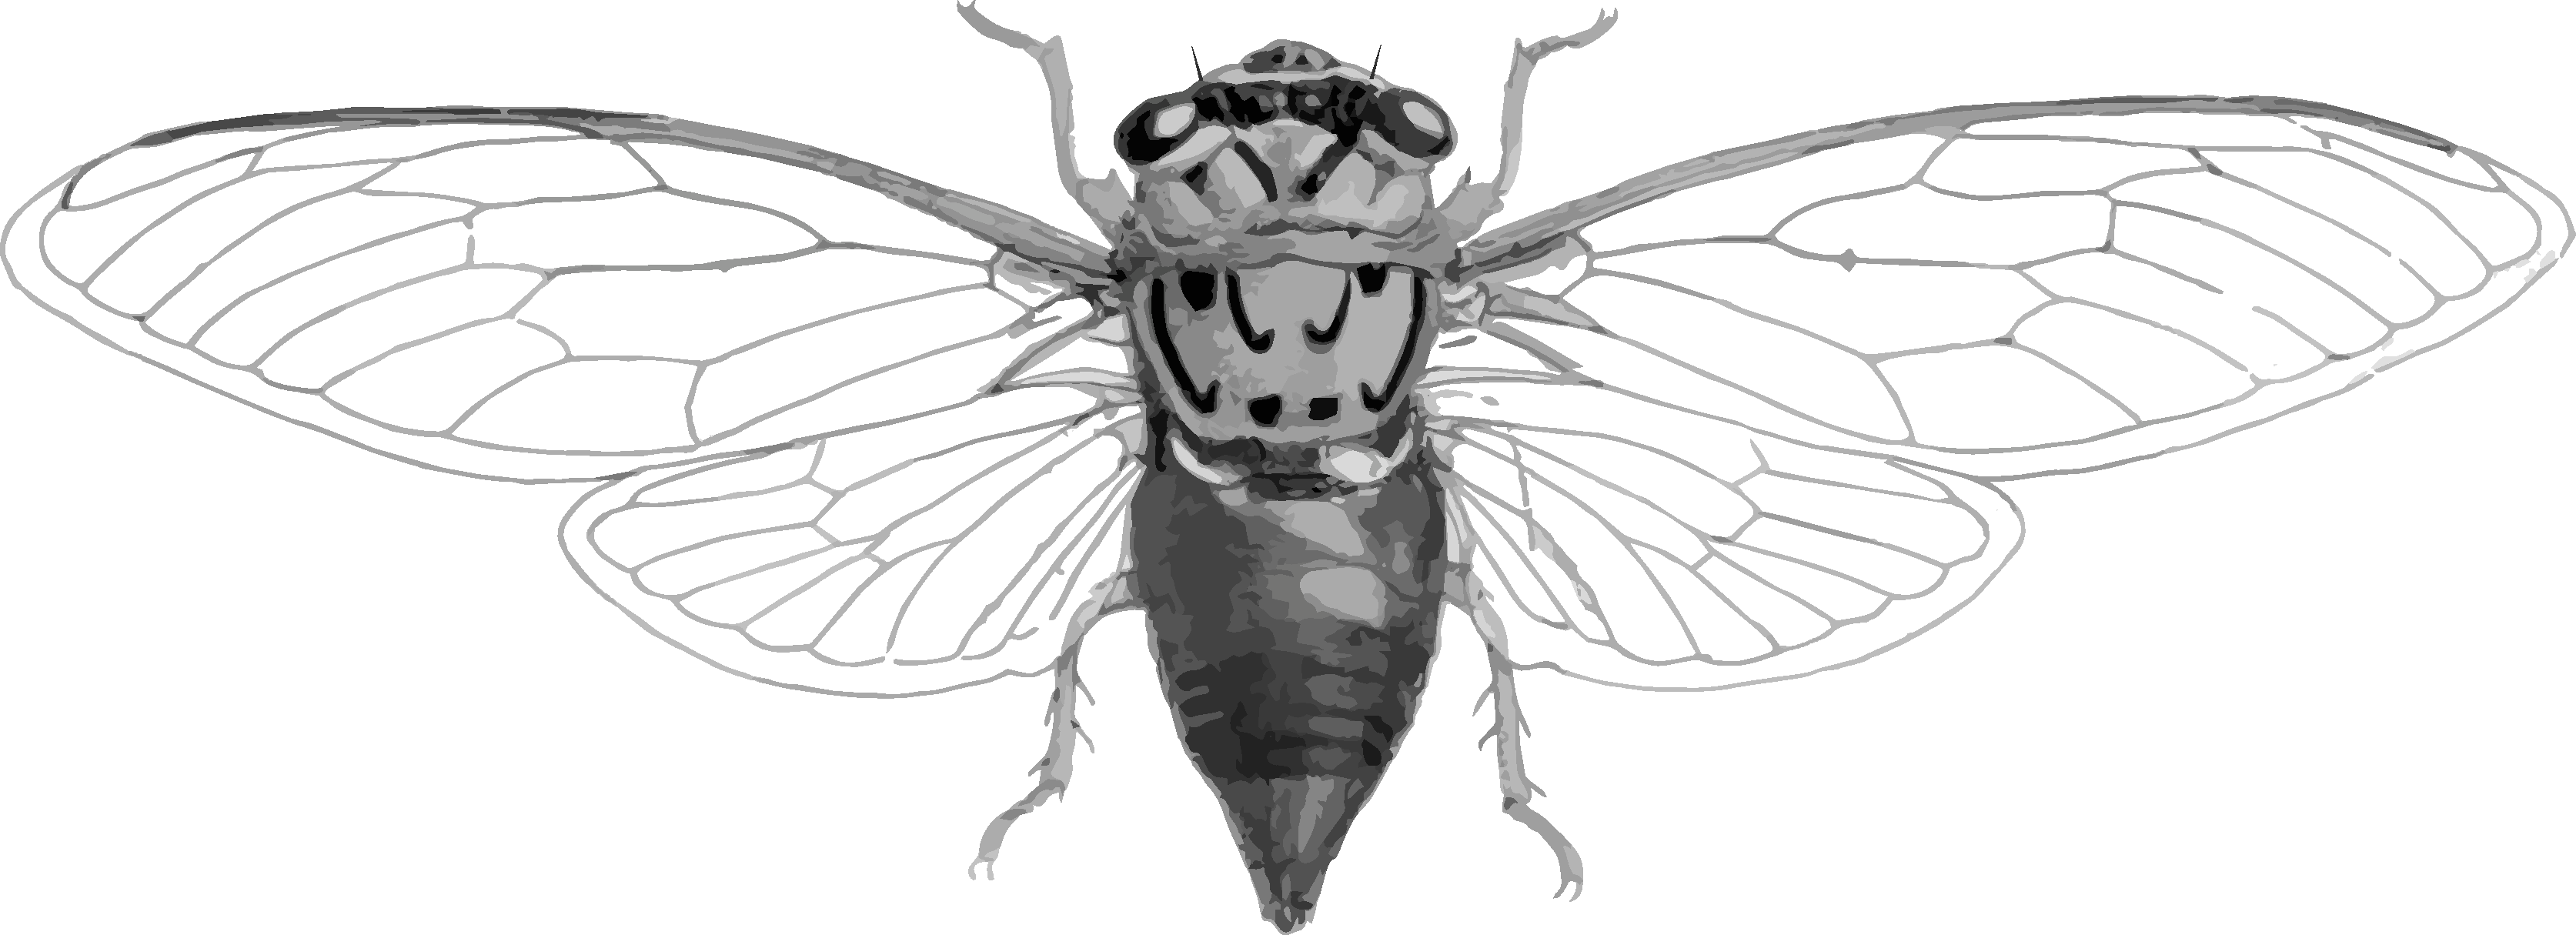
\includegraphics[width=0.75\textwidth]{acercaria/CicadidHabitus}
 \caption{Cicadidae habitus \citep[][Plate 100]{bhl33187}}
 \label{fig:cicadidae}
\end{figure}

\subsubsection{Membracidae (treehoppers)}\index{Membracidae}
\noindent{}\textit{Diagnostic characters:} Pronotum extends over abdomen; fore wing without many costal crossveins (figure \ref{fig:membrac2}; compare to Cicadidae); hind tibiae without large apical spur and without faint lateral spines.\vspace{3mm}

\noindent{}\textit{Natural history:} More than 3,000 species have been described worldwide, many of which have elaborate pronotal modifications. Treehoppers communicate with tymbals and often exhibit maternal care.\vspace{3mm}

\begin{theo}
{}Look at the variety of pronotal shapes in Membracidae. Can you think of at least three potential functions?
\end{theo} 

\begin{figure}[ht!]
 \centering
 \begin{subfigure}[ht!]{0.45\textwidth}
  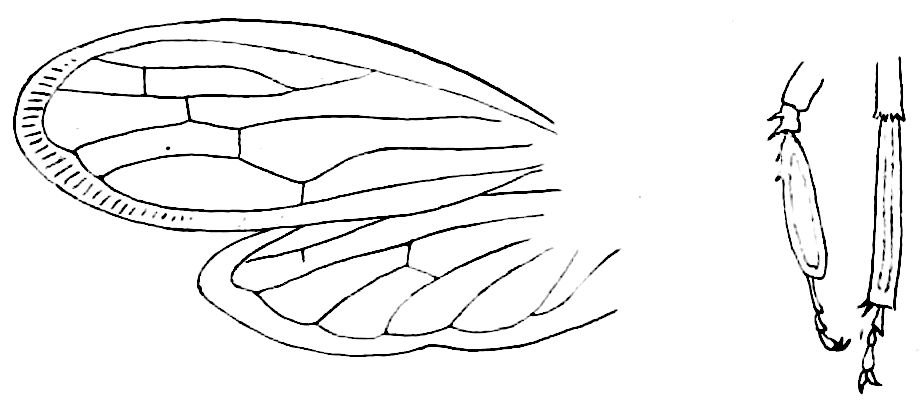
\includegraphics[width=\textwidth]{acercaria/MembracidWings}
  \caption{}
  \label{fig:membrac1}
 \end{subfigure}
 \hfill
 \begin{subfigure}[ht!]{0.45\textwidth}
  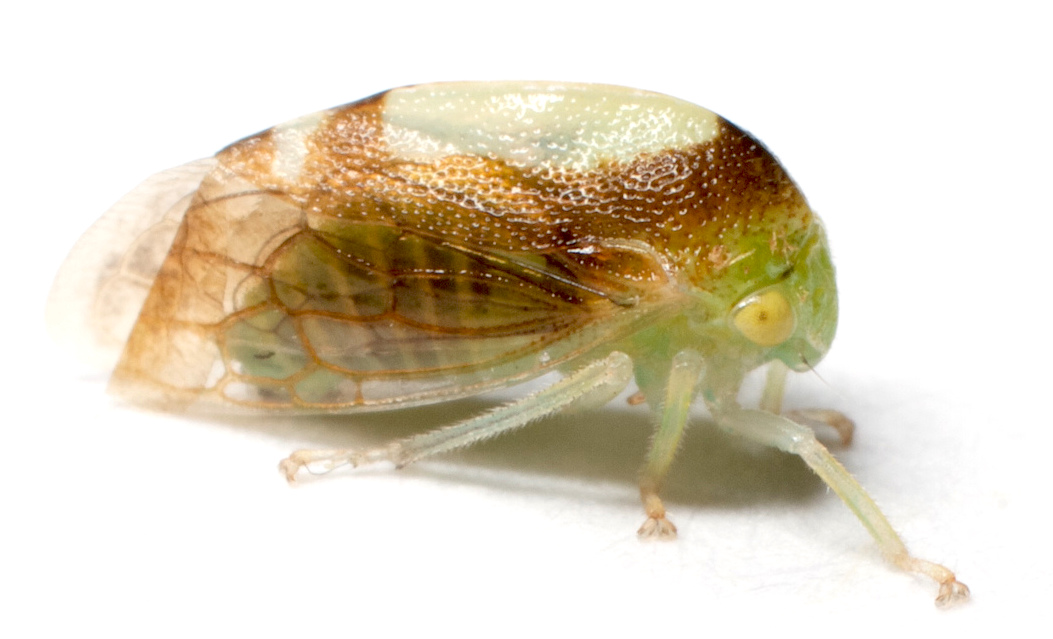
\includegraphics[width=\textwidth]{acercaria/MembracidHabitus}
  \caption{}
  \label{fig:membrac2}
 \end{subfigure}
 \caption{Membracidae. \textbf{(a)} Wings and legs \citep[][Plate I, Figs. 4c,4e]{bhl79792}; \textbf{(b)} habitus \citep[][Plate XLIV, Fig. 2]{bhlitem33127}}\label{fig:membracid}
\end{figure}

\subsubsection{Cicadellidae (leafhoppers)}\index{Cicadellidae}
\noindent{}\textit{Diagnostic characters:} Pronotum does not extend over abdomen (figure \ref{fig:cicadellids}); hind tibia with two rows of slender, elongate spines.\vspace{3mm}

\noindent{}\textit{Natural history:} Extraordinarily diverse group of auchenorrhynchans, with more than 22,000 described species, spanning from 2--30 mm in length. Leafhoppers also communicate with tymbals. Many species are important pests, including some that vector plant viruses and other disease-causing agents.\vspace{3mm}


\begin{figure}[ht!]
 \centering
  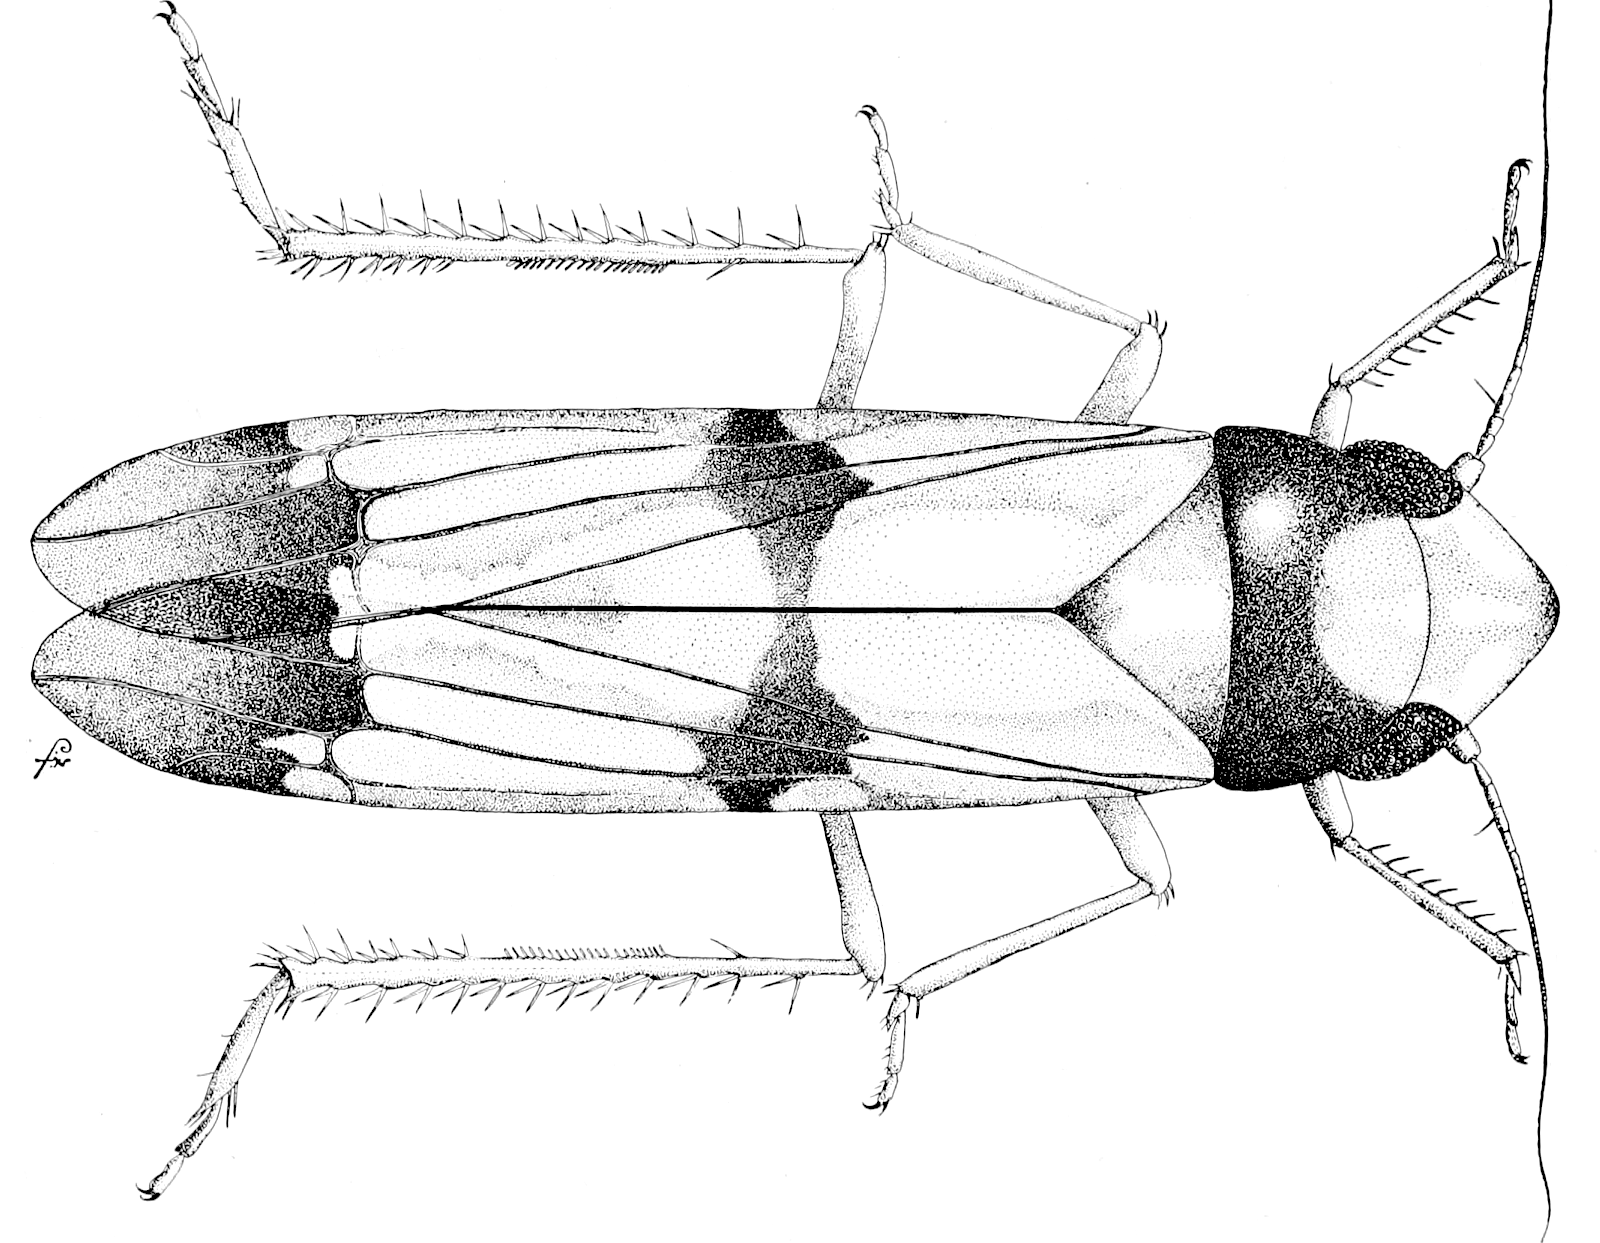
\includegraphics[width=0.45\textwidth]{acercaria/cicadellidHabitus}
  \caption{Cicadellidae habitus \citep[][Plate I]{runner1923three}}
 \label{fig:cicadellids}
\end{figure}

\subsubsection{Cercopoidea (froghoppers, spittle bugs)}\index{Cercopoidea}
\noindent{}\textit{Diagnostic characters:} hind tibiae with 1 or 2 robust lateral and numerous apical spines (figure \ref{fig:cercopid}); fore wing usually more strongly sclerotized than hind wing. The family-level classification is not yet fully resolved.\vspace{3mm}

\noindent{}\textit{Natural history:} Approximately 2,600 species have been described worldwide, most of which are understood to be xylem-feeders (unlike most other auchenorrhynchans, which are phloem-feeders). Nymphs ensconce themselves in a frothy, bubbly matrix of waste (``spittle''), where they are protected from many threats.\vspace{3mm}

\begin{figure}[ht!]
 \centering
 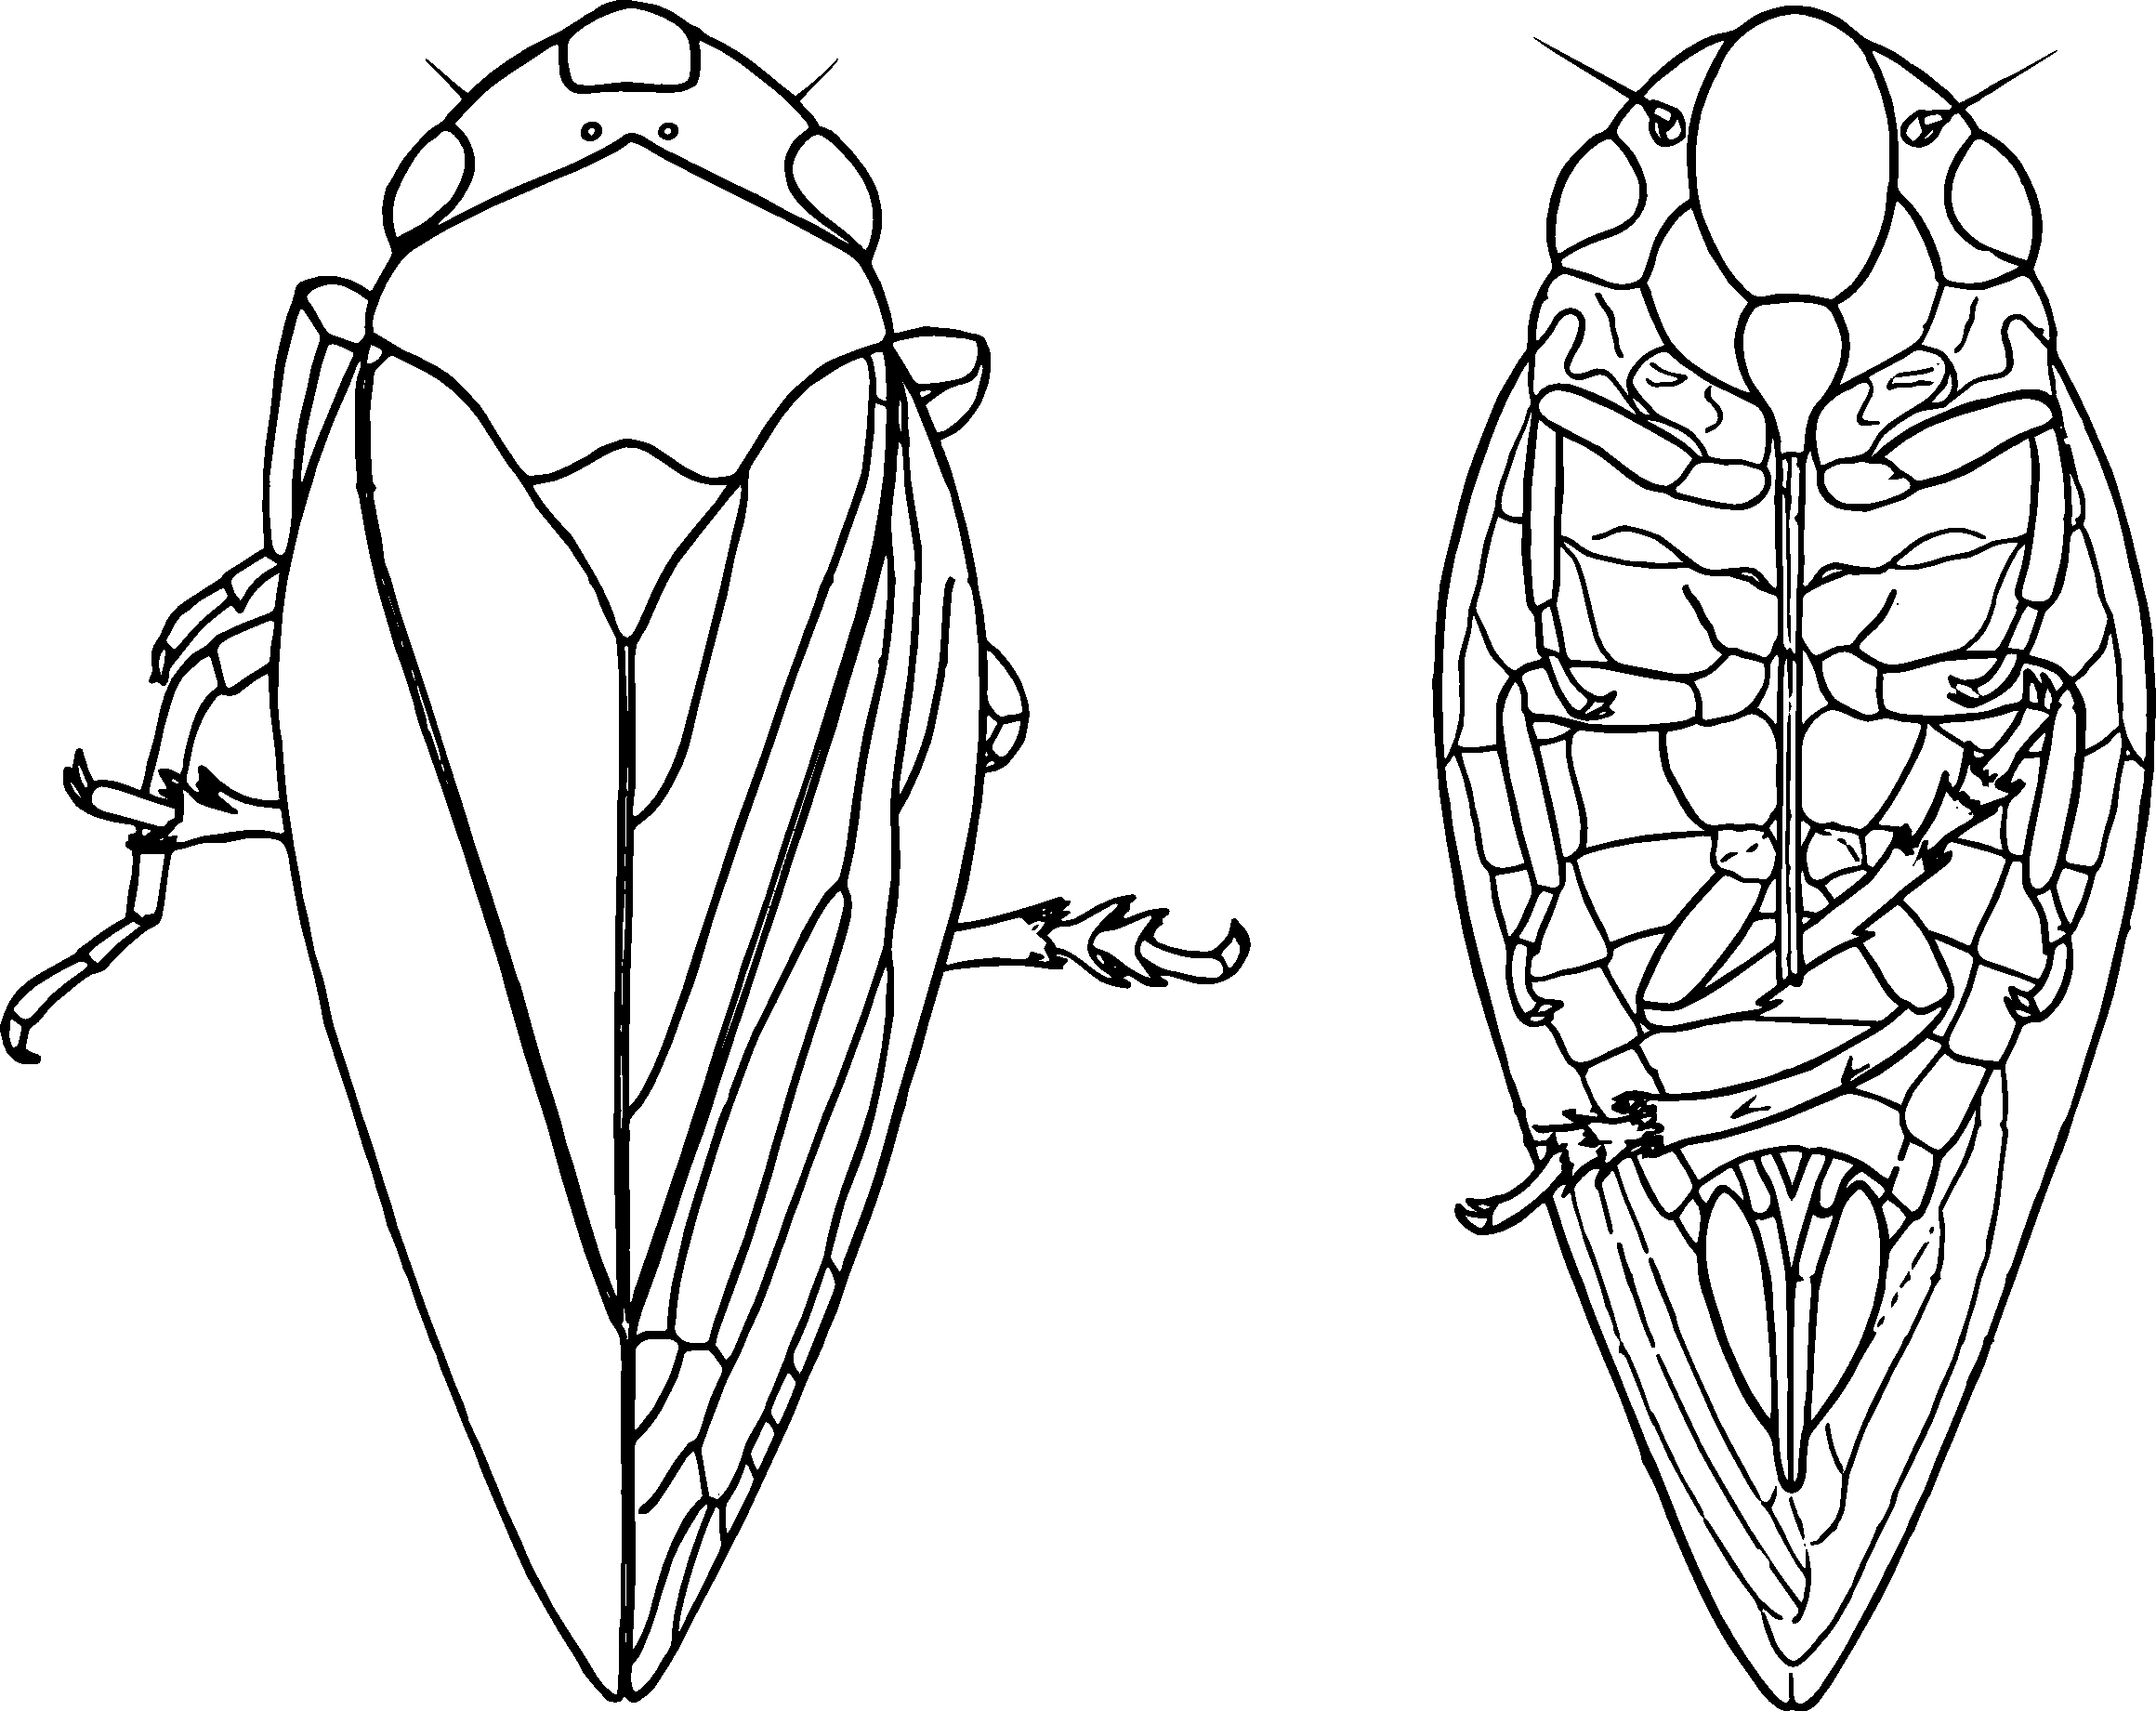
\includegraphics[width=0.55\textwidth]{acercaria/cercopoidHabitus}
 \caption{Cercopoidea habitus \citep[][Fig. 18]{bhlitem140074}}
 \label{fig:cercopid}
\end{figure}

\subsubsection*{Fulgoromorpha}

\subsubsection{Fulgoroidea (planthoppers)}\index{Fulgoroidea}
\noindent{}\textit{Diagnostic characters:} Antennae arise below eyes on sides of head; flagellum reduced to arista; median, emarginated area of the head present; fork-like vein present on fore wing anal region; body wedge-shaped, flattened from side to side, wings broad, triangular. The family-level classification is not yet fully resolved, but there are about 13 families in North America.\vspace{3mm}

\noindent{}\textit{Natural history:} More than 12,500 species are known worldwide, most of which are plant-feeders. The immature stages of some families (\textit{e.g.}, Achilidae, Derbidae) feed on fungi. This is the only superfamily in Fulgoroidea, and it currently includes about 20 families. Common taxa include Delphacidae, Dictyopharidae, Flatidae, and Fulgoridae.\vspace{3mm}

\begin{figure}[ht!]
 \centering
 \begin{subfigure}[ht!]{0.5\textwidth}
  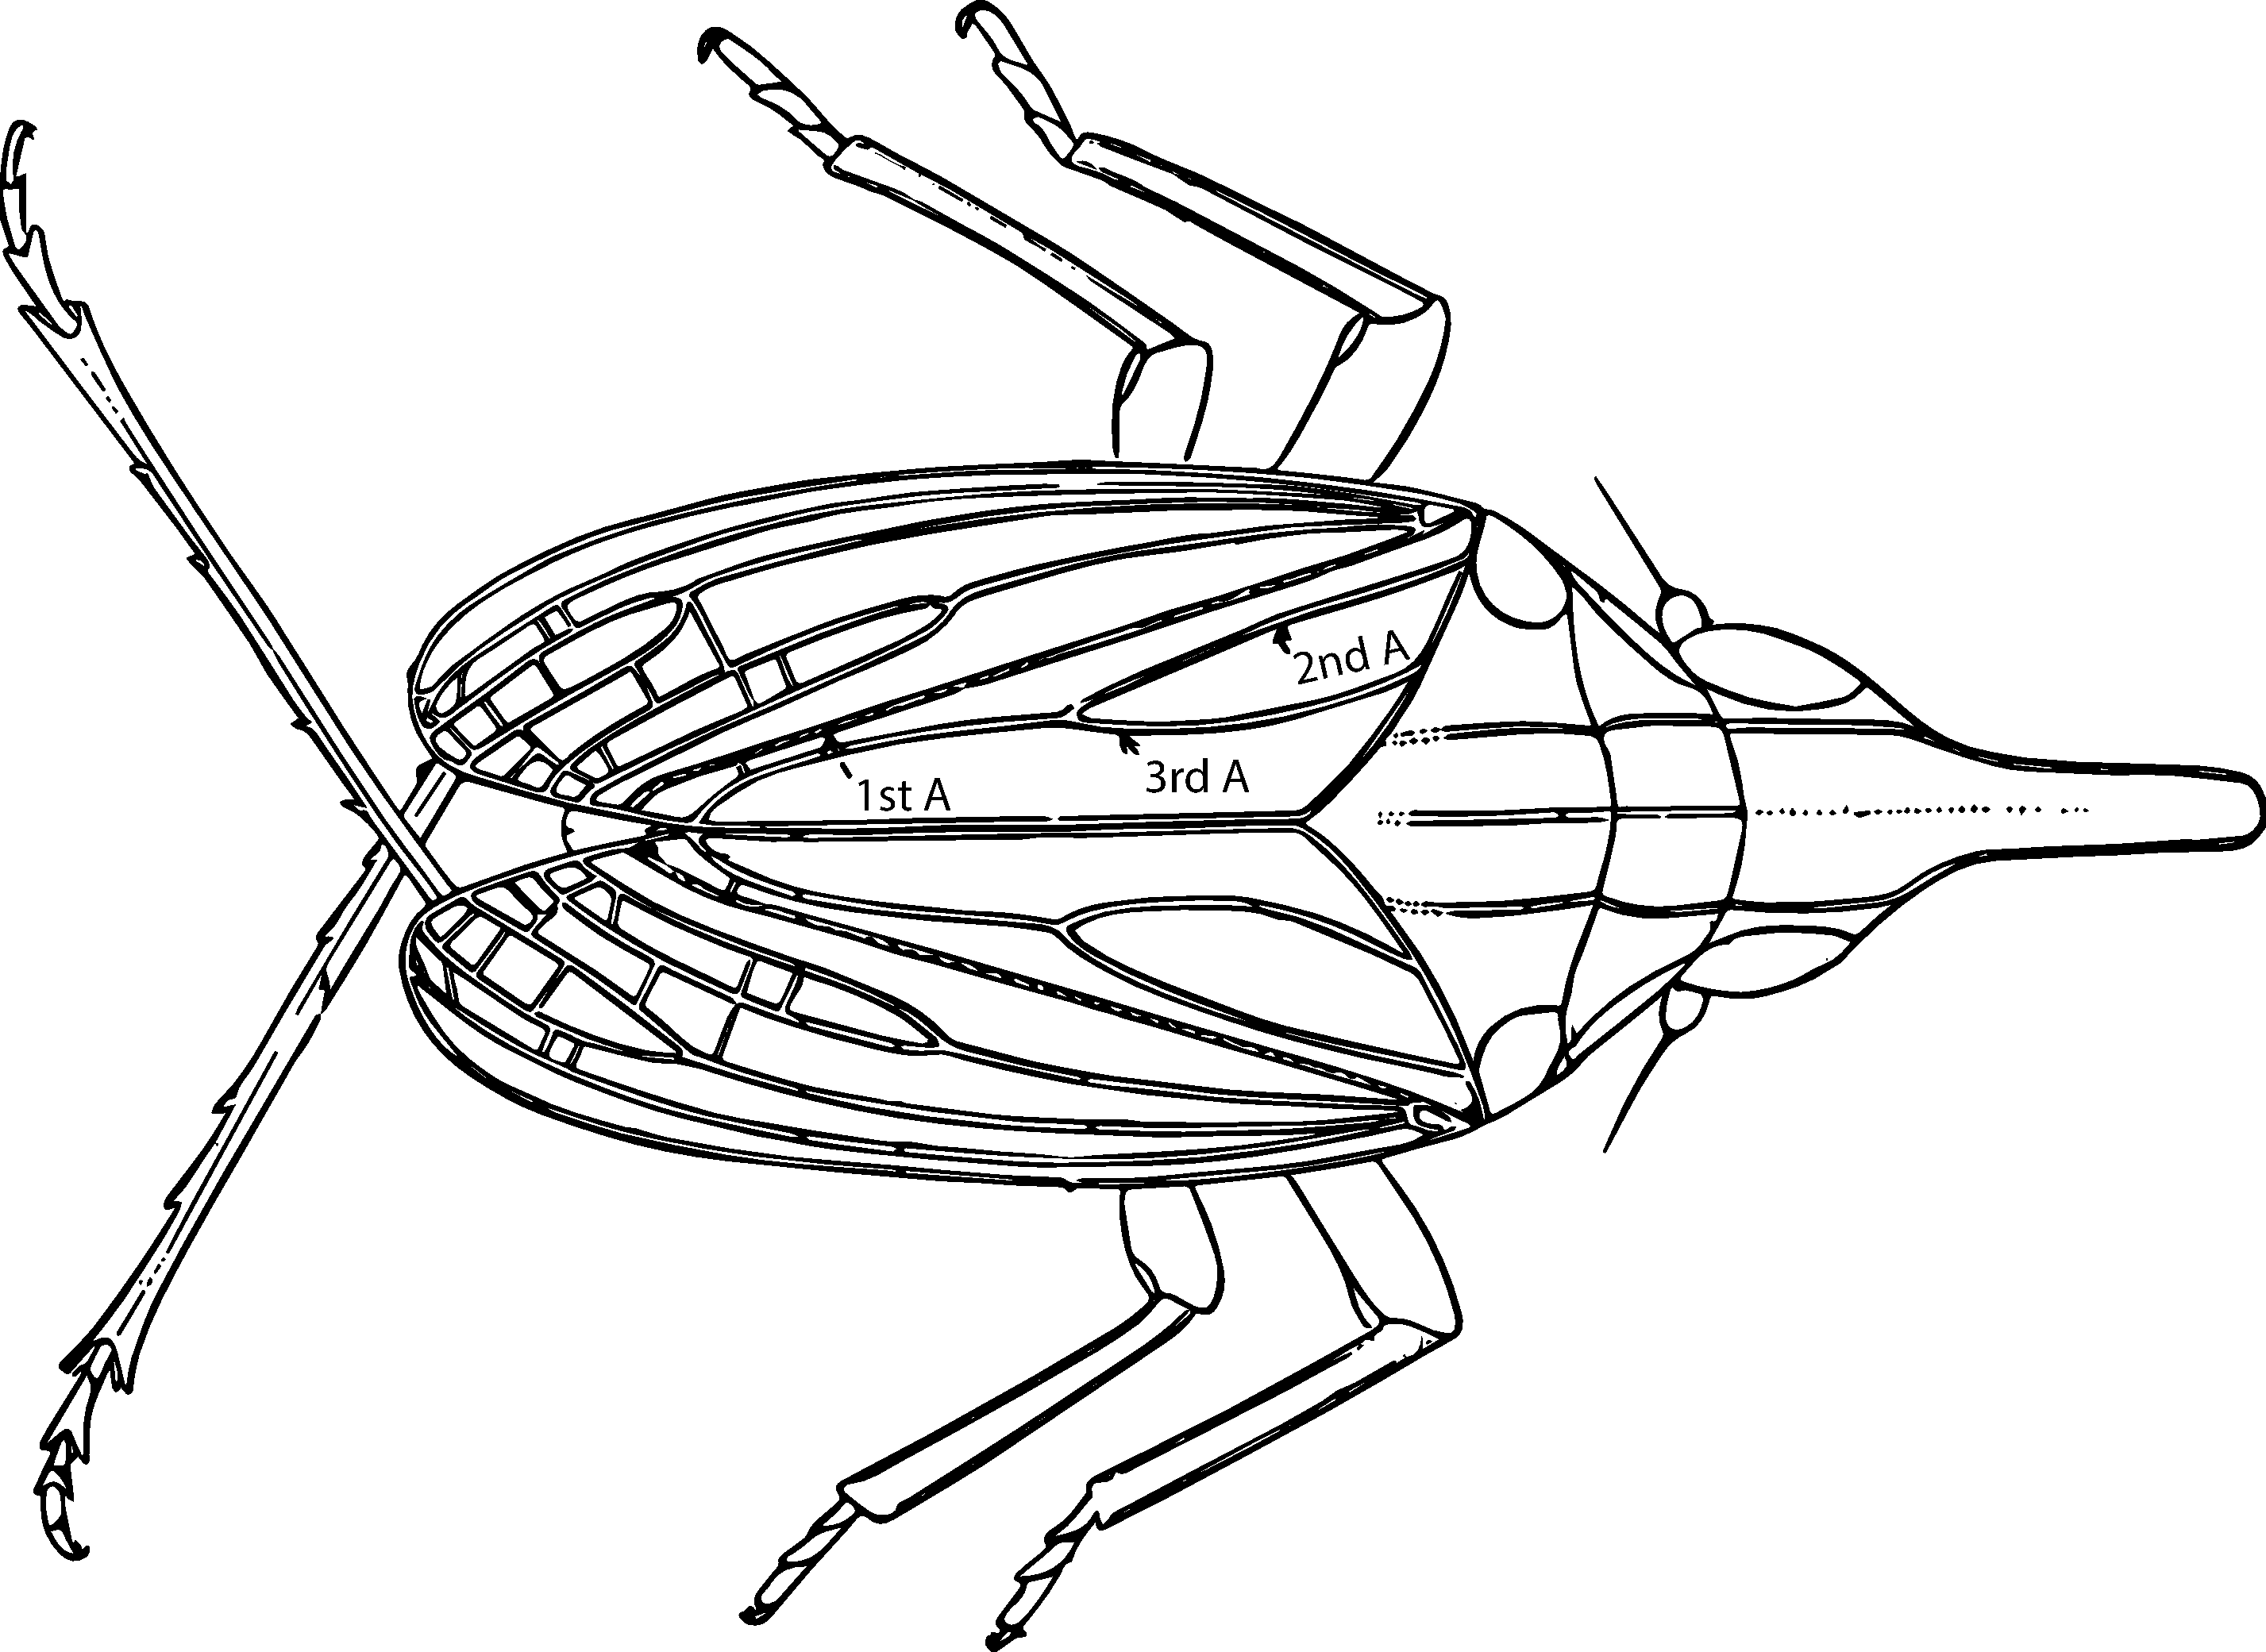
\includegraphics[width=\textwidth]{acercaria/fulgoroid}
  \caption{}
  \label{fig:fulgoroid}
 \end{subfigure}
 \hfill
 \begin{subfigure}[ht!]{0.4\textwidth}
  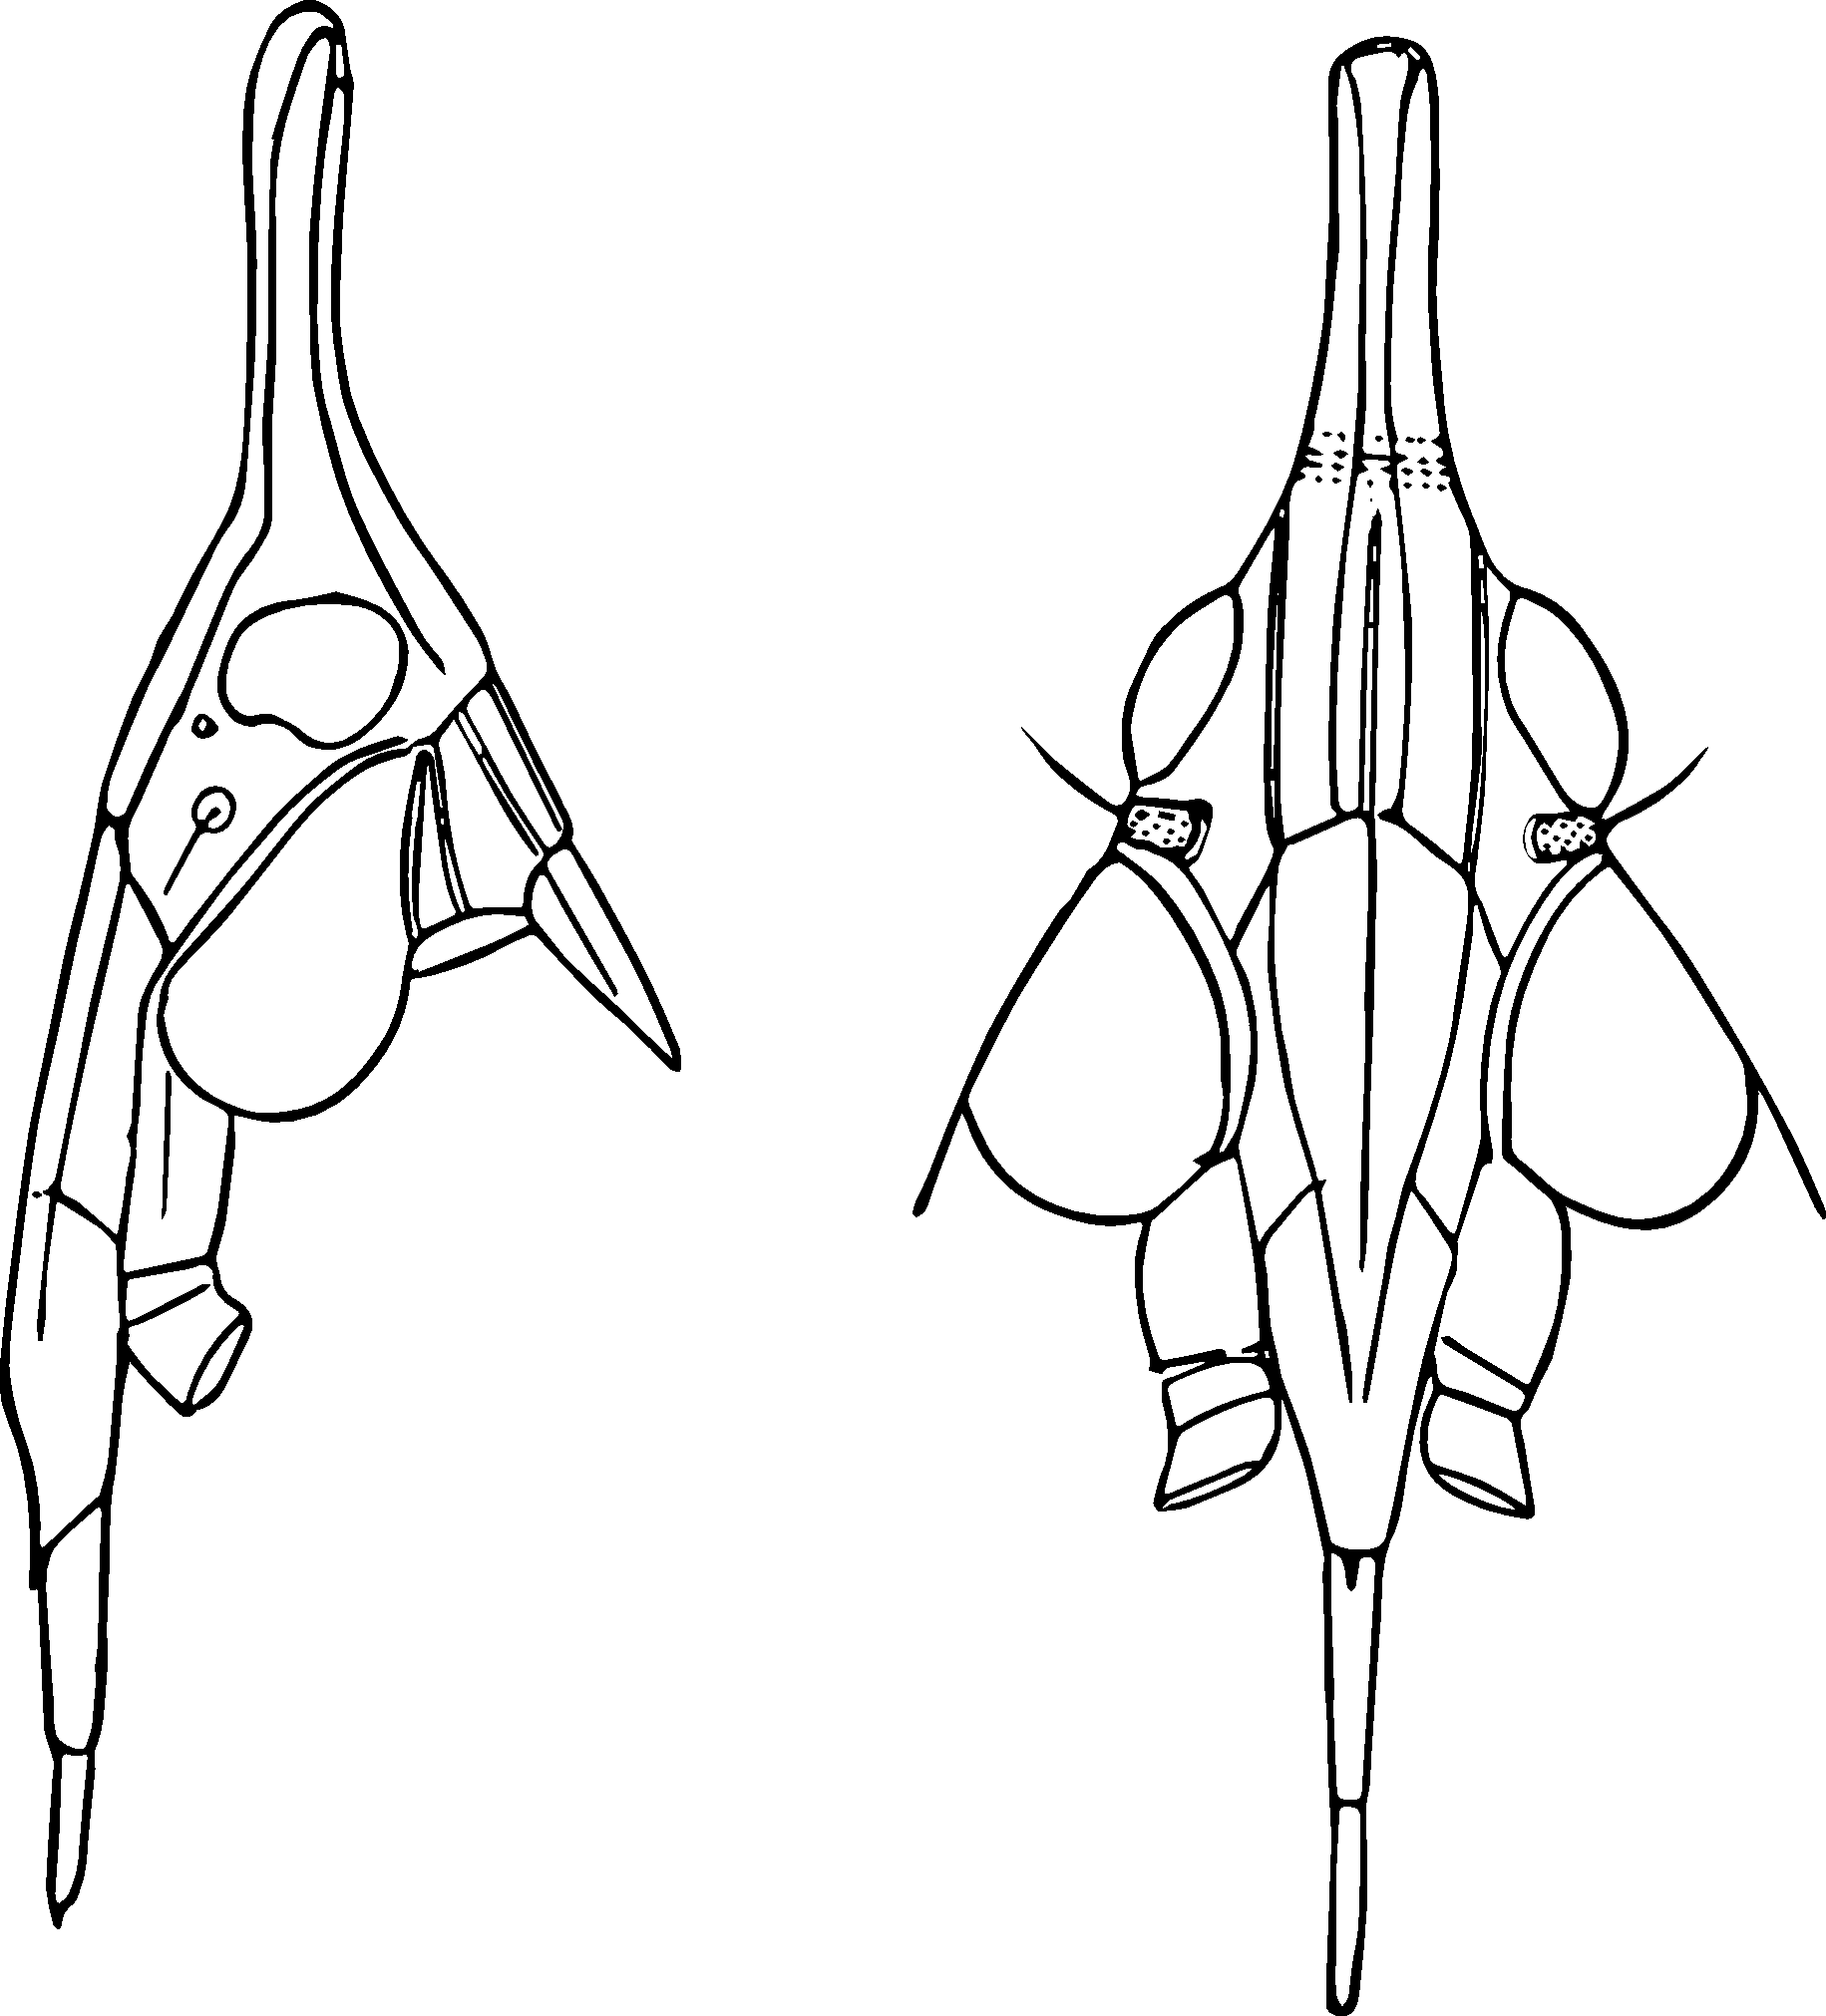
\includegraphics[width=\textwidth]{acercaria/fulgoroidHead}
  \caption{}
  \label{fig:fulgoroidHead}
 \end{subfigure}
 \caption{Fulgoroidea. \textbf{(a)} Habitus \citep[Modified from][Fig. 1]{britton1923hemiptera}; \textbf{(b)} head \citep[Modified from][Fig. 2]{britton1923hemiptera}}\label{fig:fulgoroidea}
\end{figure}

\subsection{Coleorrhyncha (moss bugs)}\index{Coleorrhyncha}
This suborder has a Gondwanic distribution, being found today only in southern South America, Australia, New Caledonia, and New Zealand. There is a single extant family, Peloridiidae, with about 35 described species.

\begin{figure}[ht!]
 \centering
 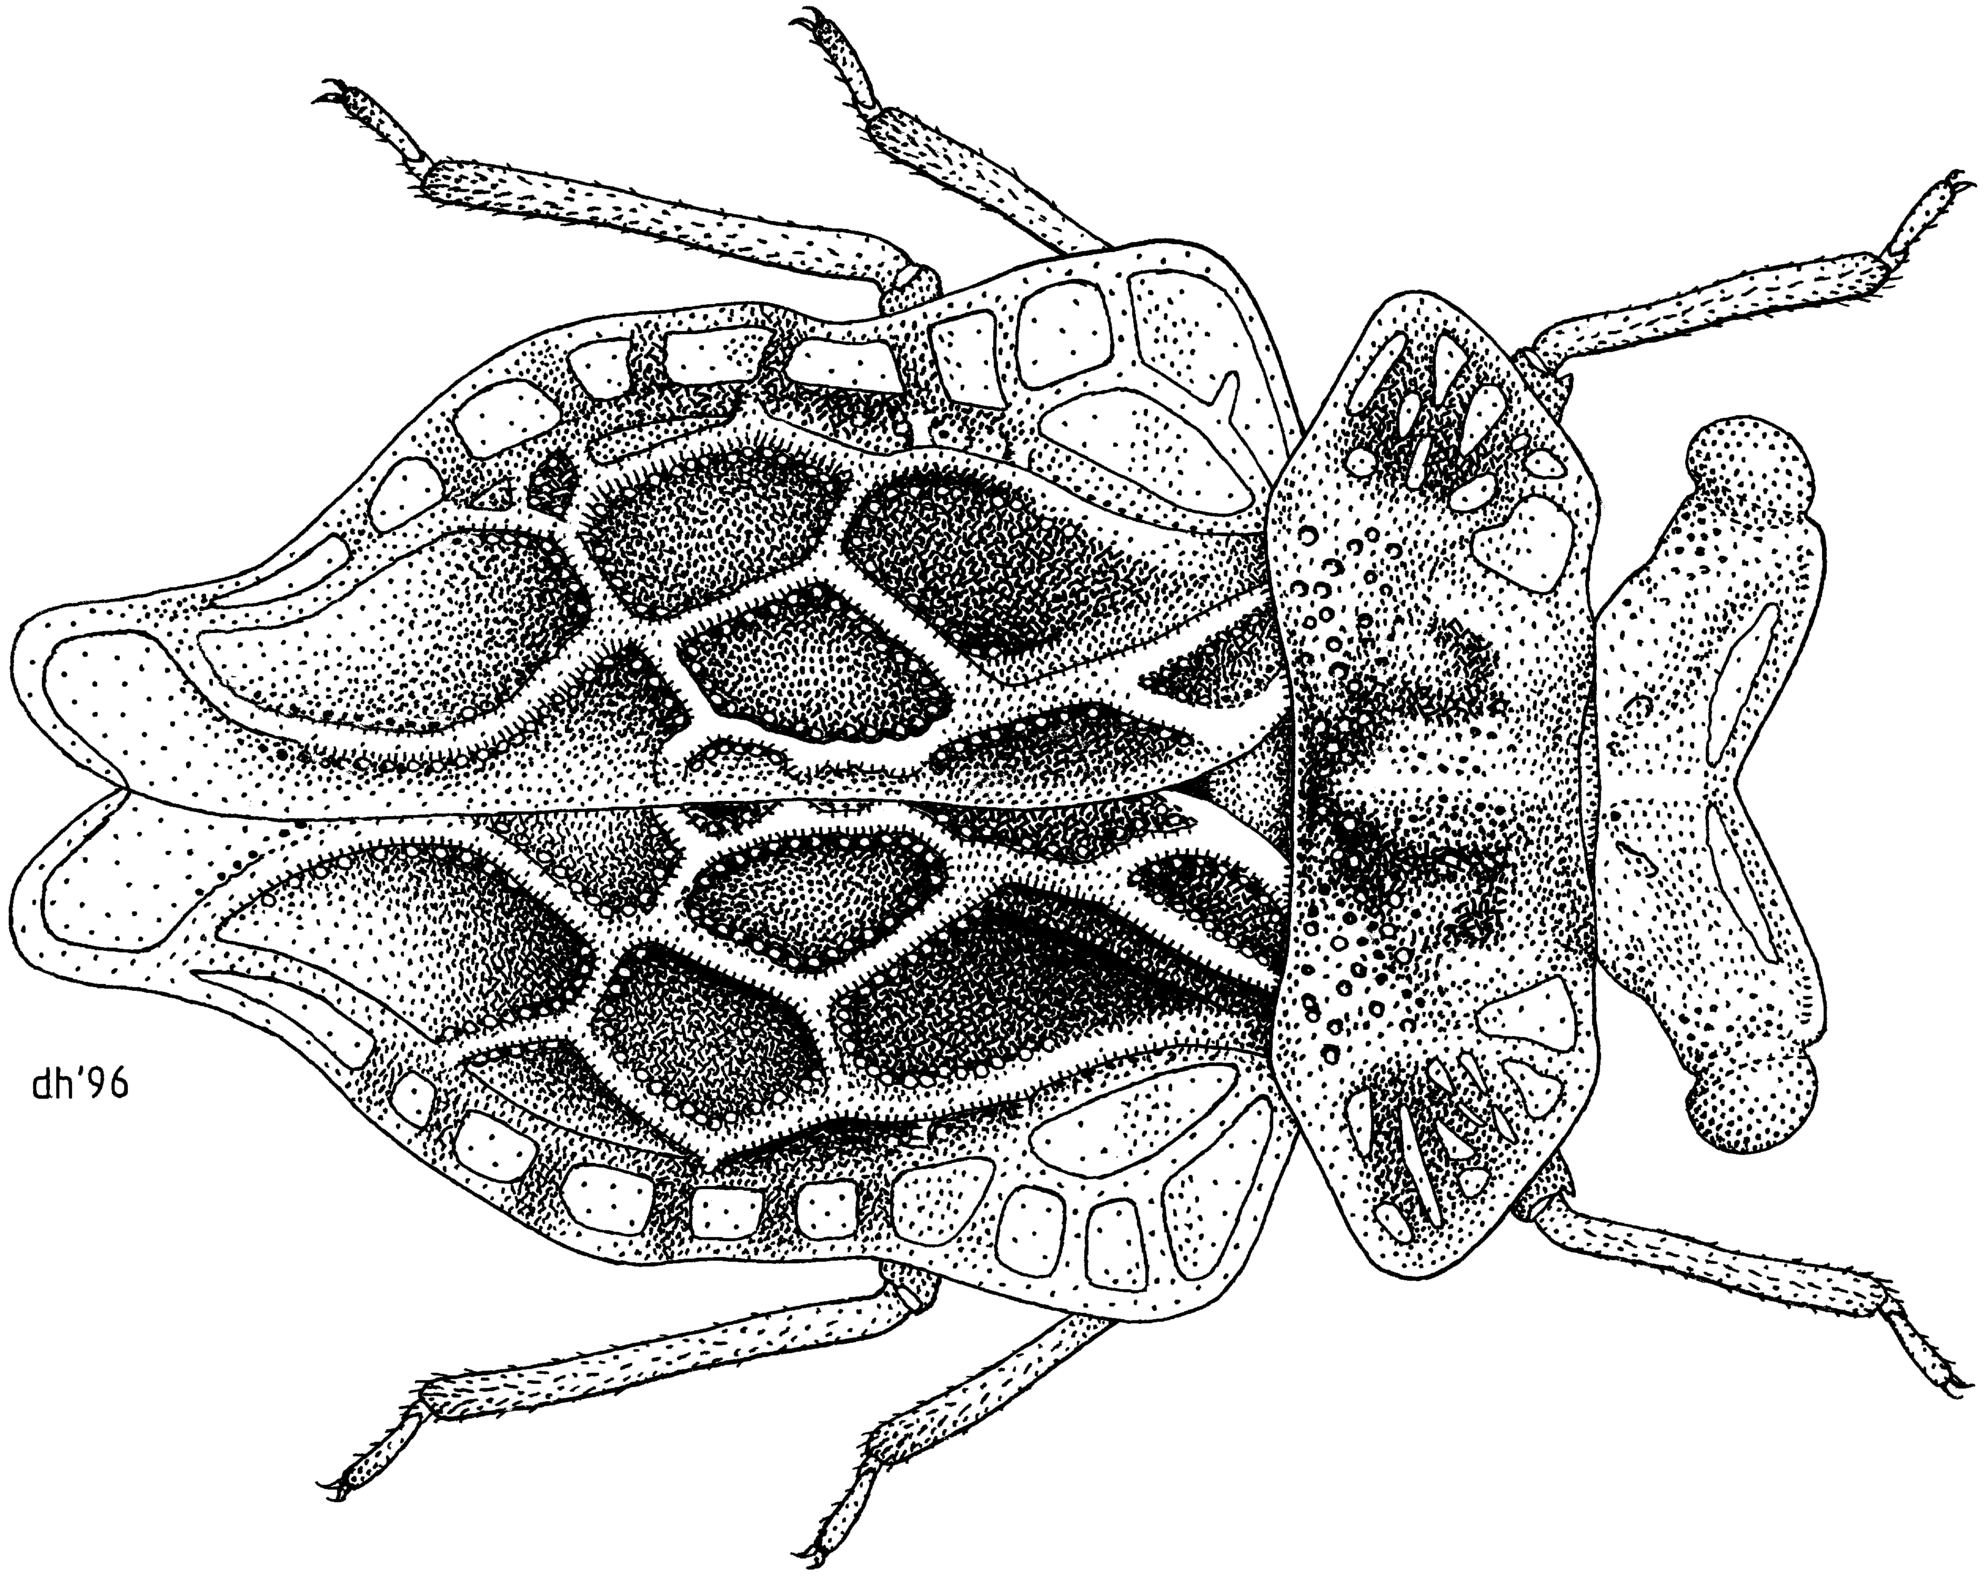
\includegraphics[width=0.4\textwidth]{acercaria/Coleorrhyncha}
 \caption{Coleorrhyncha (modified from illustration (CC BY 4.0 International) by Des Helmore / Manaaki Whenua – Landcare Research)}
 \label{fig:coleorrhyncha}
\end{figure}

\subsection{Heteroptera (true bugs)}\index{Heteroptera}
A suborder of Hemiptera commonly referred to as ``true bugs'', which can be recognized by the following characters:
\begin{itemize}
    \item head prognathous, mouthparts arises anteriorly from head in lateral view; there is a distinct distance between the labium and the procoxae, compared to other hemipterans
    \item antennae filiform
    \item anterior part of fore wing is more sclerotized than posterior part of fore wing and the hind wing (\latinword{hemelytra})
    \item tarsi with usually 3 tarsomeres, rarely 2 or 4
    \item absence of a complex tymbal acoustic system on abdominal segment I
    \item \latinword{scent gland} (sgo) on the metathorax usually present (but see Rhopalidae)
\end{itemize}

\subsubsection{Enicocephalomorpha}\index{Enicocephalomorpha}
This infraorder contains a single extant family.

\subsubsection{Enicocephalidae (unique-headed bugs)}\index{Enicocephalidae}
\noindent{}\textit{Diagnostic characters:} Body slim; ocelli present; antennae and beak 4-segmented; fore wings mostly membranous; front femur and tarsus relatively enlarged; mid and hind tarsus each 2-segmented.\vspace{3mm}

\noindent{}\textit{Natural history:} Approximately 400 species have been described worldwide, and most are between 2--4 mm long. They are often found in swarms, which gives them their other common name: gnat bugs. They are though to be predators of invertebrates that live in leaf litter and under logs.\vspace{3mm}

\begin{figure}[ht!]
 \centering
 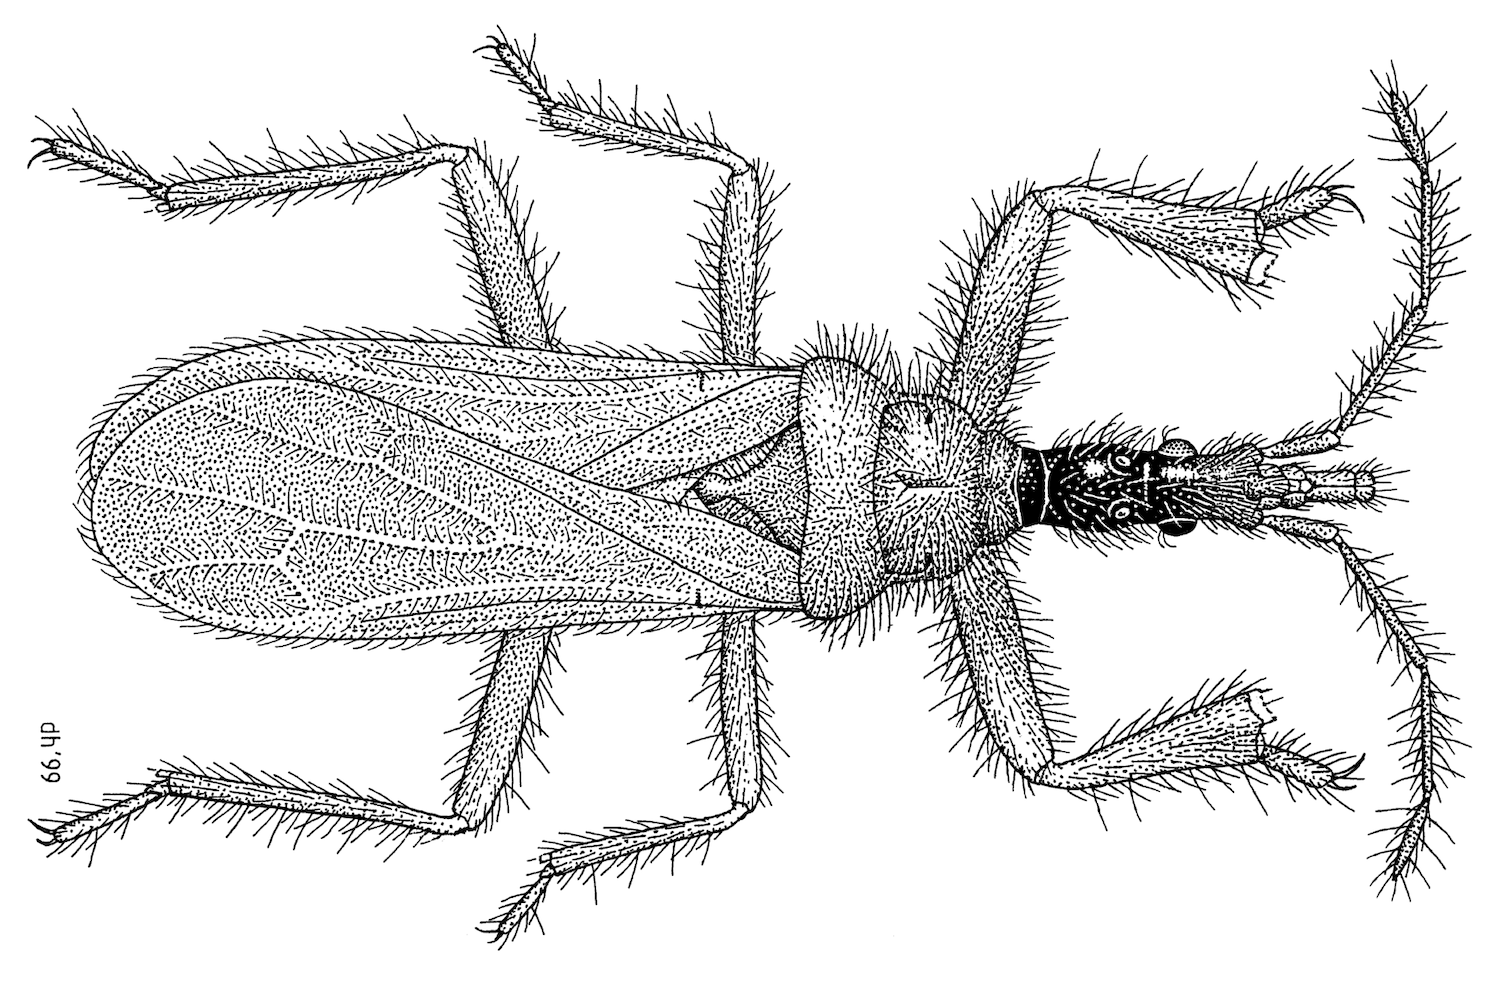
\includegraphics[width=0.5\textwidth]{acercaria/Enicocephalidae}
 \caption{Enicocephalidae habitus. Photo (CC BY 4.0) by Des Helmore, Manaaki Whenua / Landcare Research}
 \label{fig:enicocephalid}
\end{figure}

\subsubsection{Nepomorpha}\index{Nepomorpha}
This infraorder includes more than 10 families, whose species are primarily aquatic.

\subsubsection{Gelastocoridae (toad bugs)}\index{Gelastocoridae}%no need to sight ID? def in PA but NONE in collection
\noindent{}\textit{Diagnostic characters:} Body usually \textless{}10 mm long, toad-like, cryptic (camouflaged); antennae shorter than head, hidden; ocelli present; flattened, bulging eyes (figure \ref{fig:gelasto1}); fore legs shorter than mid legs.\vspace{3mm}

\noindent{}\textit{Natural history:} Approximately 100 species are known worldwide, all of which are predators. Most species are found close to aquatic habitats (\textit{e.g.} lake shores) and have cryptic coloration. The common name derives from their vaguely toad-like appearance and hopping locomotion.\vspace{3mm}

\begin{figure}[ht!]
 \centering
 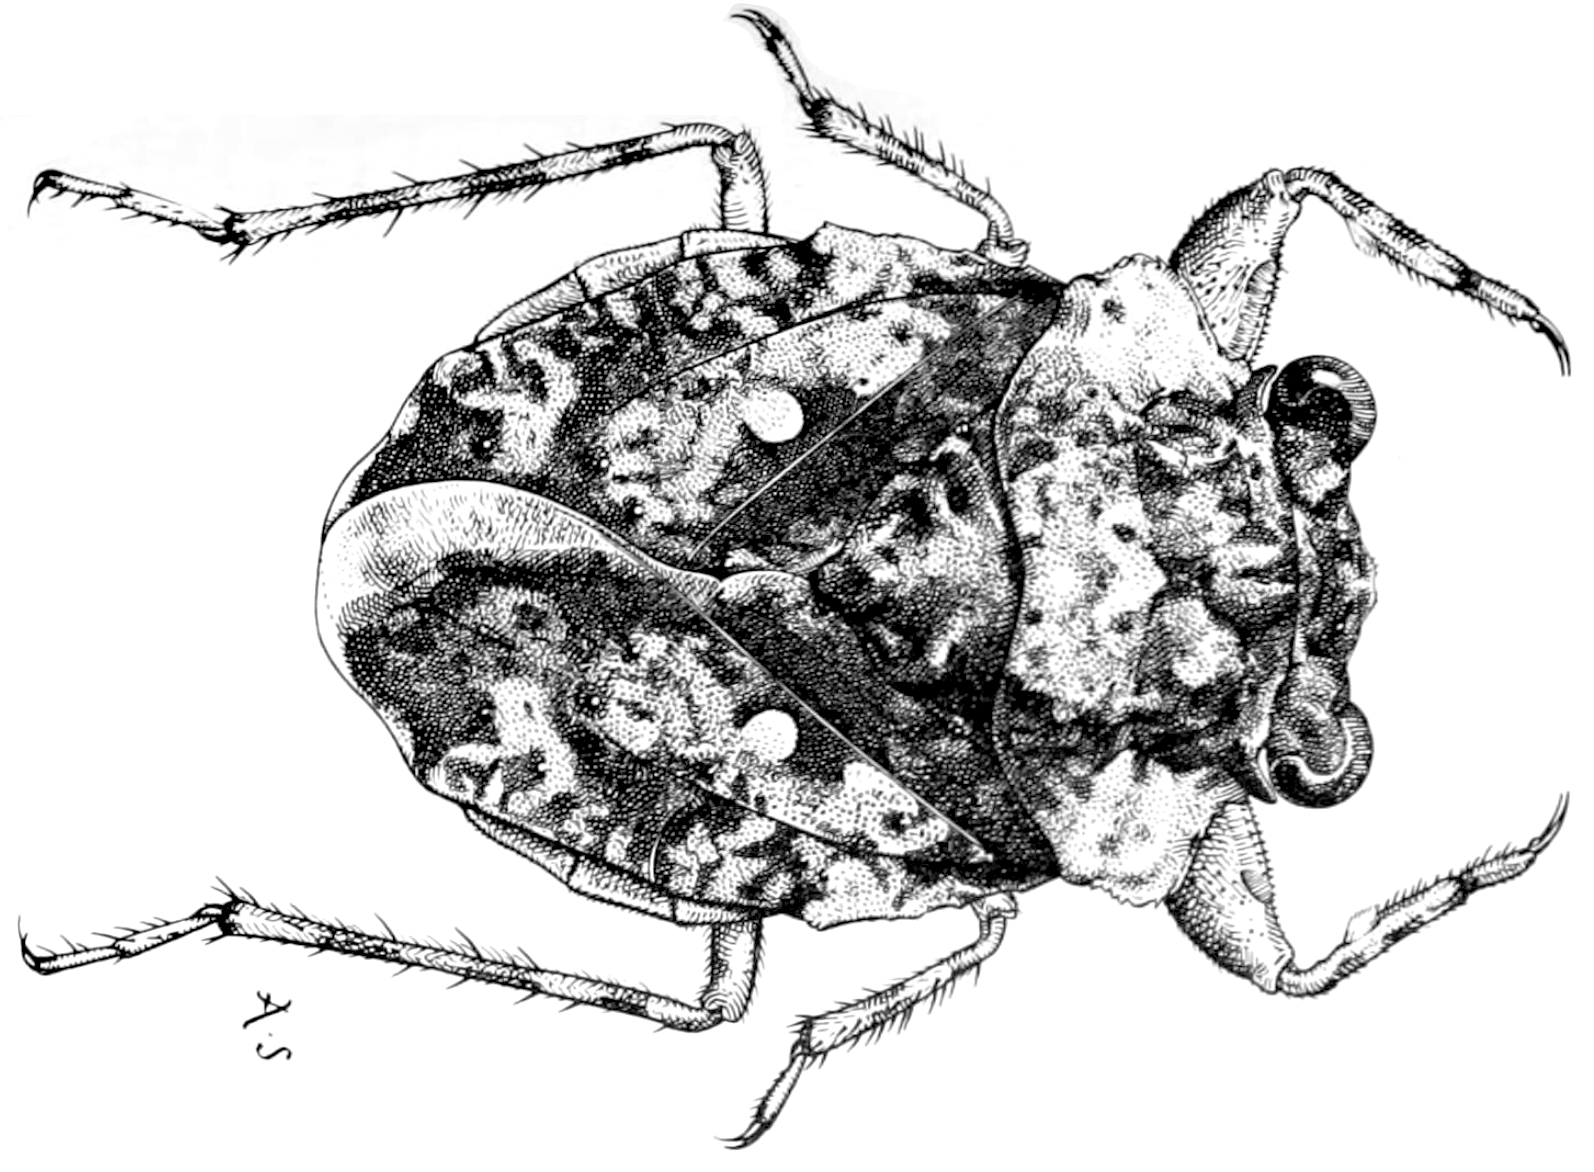
\includegraphics[width=0.4\textwidth]{acercaria/gelastocorid}
 \caption{Gelastocoridae habitus. \citep[][Fig. 7:21a]{bhlitem126080aquatic}}
 \label{fig:gelasto1}
\end{figure}

\subsubsection{Corixidae (water boatmen)}\index{Corixidae}
\noindent{}\textit{Diagnostic characters:} Body flattened dorsally, with dark pattern of thin stripes; antennae shorter than head; ocelli absent; beak very short, appears 1-segmented (figure \ref{fig:corix1}); fore legs not raptorial, fore tarsi 1-segmented and scoop-shaped (figure \ref{fig:corix1}); hind legs elongate, oar-like, hind tarsi without claws.\vspace{3mm}

\noindent{}\textit{Natural history:} Around 500 species are known worldwide, all of which are aquatic. Often they occur in great abundance and are even harvested by people for food.\vspace{3mm}

\begin{figure}[ht!]
 \centering
 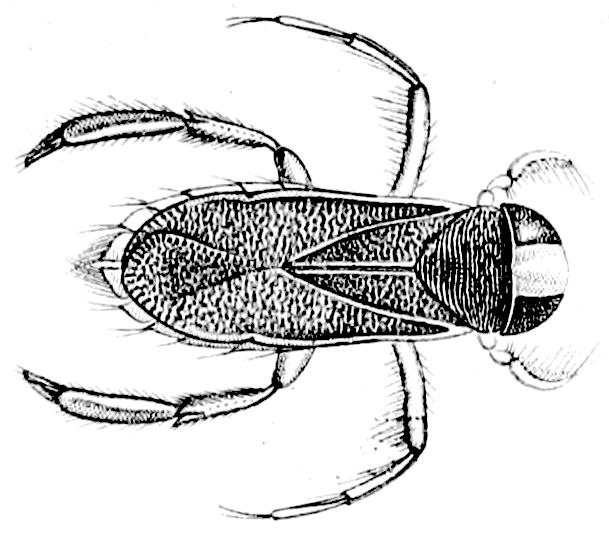
\includegraphics[width=0.35\textwidth]{acercaria/CorixidHabitus}
 \caption{Corixidae dorsal habitus \citep[][Plate 7, Fig. 5]{bhl37902}}
 \label{fig:corix1}
\end{figure}

\begin{theo}
{}Compare the mouthparts of Corixidae to the other heteropterans. What do you think Corixidae eat, based on the morphology of the mouthparts? Hint: Check out their fore legs.\vspace{3mm}

\noindent{}Most corixids are patterned with stripes. What might their function be?
\end{theo}

\subsubsection{Notonectidae (backswimmers)}\index{Notonectidae}
\noindent{}\textit{Diagnostic characters:} Body convex dorsally, mottled, light-colored (figure \ref{fig:notonect1}); antennae shorter than head; ocelli absent; fore legs not raptorial, front tarsi not scoop-shaped; hind legs elongate, oar-like, hind tarsi without claws.\vspace{3mm}

\noindent{}\textit{Natural history:} Approximately 400 species are known worldwide, all of which are predators. These insects can deliver a painful bite(!) when handled. They also communicate via stridulation, and scraper/file morphology can be diagnostic.\vspace{3mm}

\begin{figure}[ht!]
 \centering
 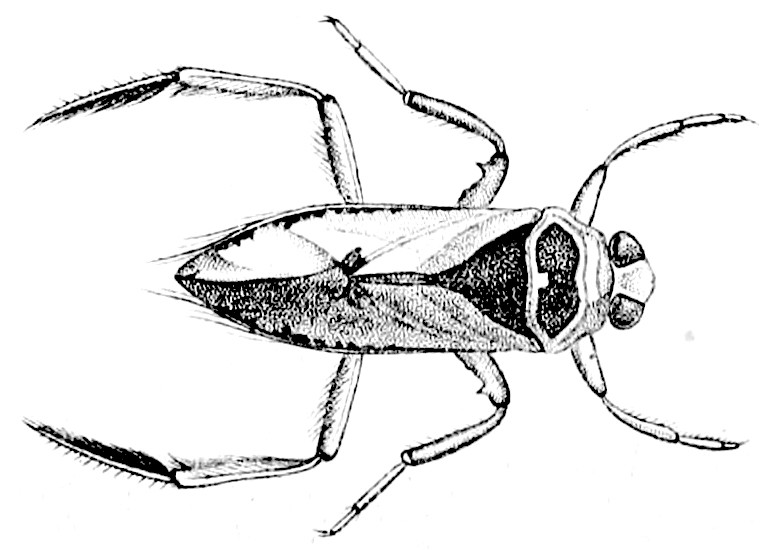
\includegraphics[width=0.45\textwidth]{acercaria/NotonectidHabitus}
 \caption{Notonectidae, dorsal habitus \citep[][Plate 7, Fig. 2]{bhl37902}}
 \label{fig:notonect1}
\end{figure}

\subsubsection{Nepidae (water scorpions)}\index{Nepidae}
\noindent{}\textit{Diagnostic characters:} Body shape variable (figure \ref{fig:nepid1}); antennae shorter than head; ocelli absent; tarsi each comprised of 1 tarsomere; fore legs raptorial; hind legs not oarlike, hind tarsi with claws; 2 long terminal abdominal appendages called ``airstraps''.\vspace{3mm}

\noindent{}\textit{Natural history:} Almost 300 species have been described worldwide. All are predators of other aquatic organisms, mainly invertebrates. They breathe through a snorkel-like structure, the air straps, located off the apex of the abdomen.\vspace{3mm}

\begin{figure}[ht!]
 \centering
 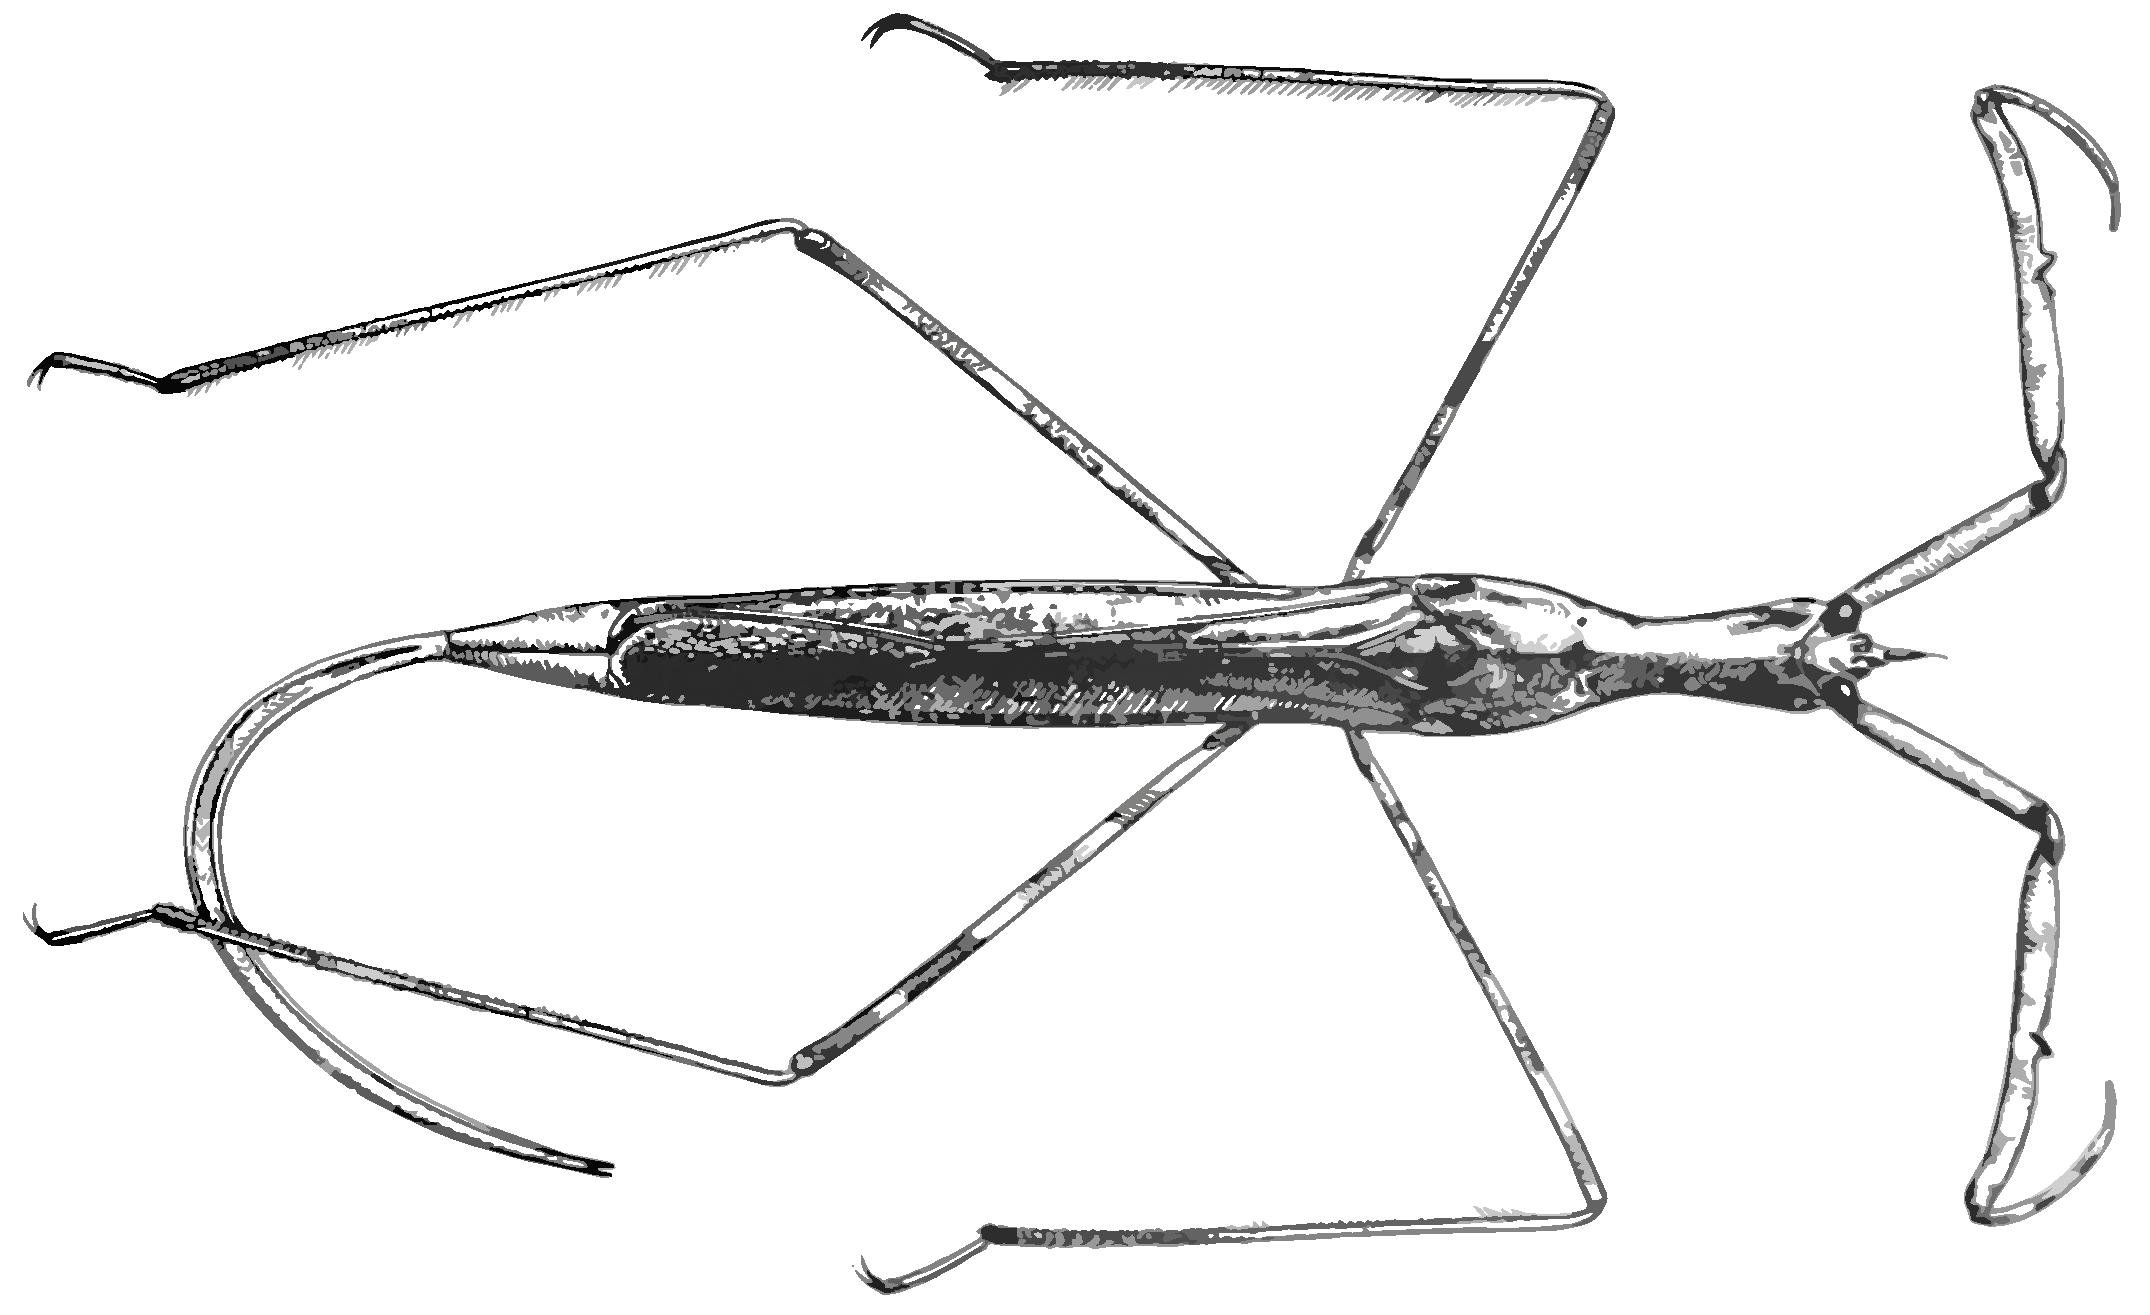
\includegraphics[width=0.55\textwidth]{acercaria/nepid}
 \caption{Nepidae, dorsal habitus \citep[Modified from Fig. 7:19 in][]{bhlitem126080aquatic}}
 \label{fig:nepid1}
\end{figure}

\subsubsection{Belostomatidae (giant water bugs)}\index{Belostomatidae}
\noindent{}\textit{Diagnostic characters:} Body large, dorso-ventrally flattened usually over \textgreater20 mm; antennae shorter than head; ocelli absent; fore legs raptorial (figure \ref{fig:belostom1}); hind legs flat, oar-like, hind tarsi with claws; membrane of fore wing with veins.\vspace{3mm}

\noindent{}\textit{Natural history:} Almost 160 species have been described worldwide, all of which are aquatic predators. In some species the female lays her eggs on the male's dorsum, and he affords the clutch some level of paternal care. These insects are mostly found in lentic environments.\vspace{3mm}

\begin{figure}[ht!]
 \centering
 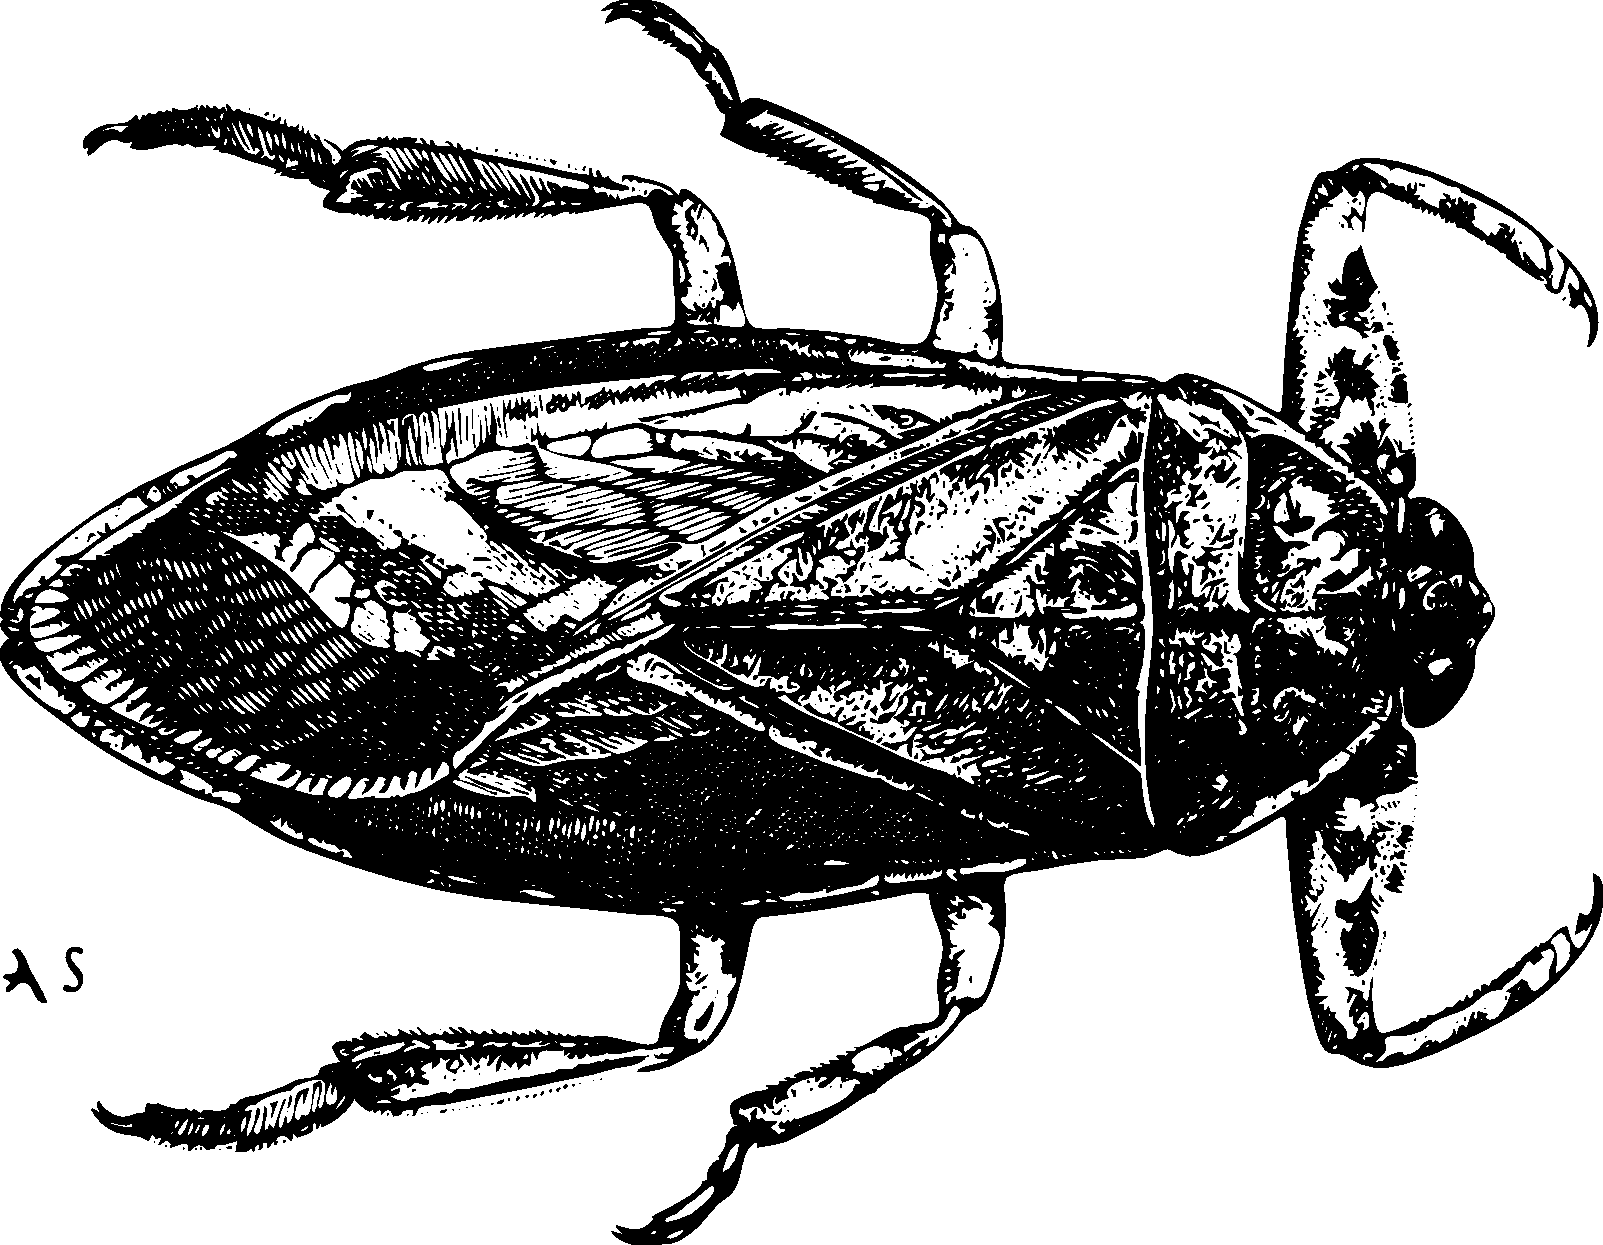
\includegraphics[width=0.45\textwidth]{acercaria/belostomatidae}
 \caption{Belostomatidae, dorsal habitus. \citep[Modified from Fig.7:17 in ][]{bhlitem126080aquatic}}
 \label{fig:belostom1}
\end{figure}

\begin{theo}
{}Describe some of the adaptations you see in the previous two families for predation. Can you predict how they hunt and capture prey?\vspace{3mm}

\noindent{}Look closely at the tarsi and the apex of each leg on the following two families. Do you see any adaptations that might be related to their semi-aquatic lifestyle?
\end{theo}

\subsubsection{Gerromorpha}\index{Gerromorpha}
This infraorder includes almost 10 families, whose species are semi-aquatic and adapted primarily for living on the surface of water.

\subsubsection{Gerridae (water striders)}\index{Gerridae}
\noindent{}\textit{Diagnostic characters:} Body usually \textgreater5 mm; antennae longer than head; middle legs arising closer to hind legs than to front legs (figure \ref{fig:gerrid1}); hind femur longer than abdomen.\vspace{3mm}

\noindent{}\textit{Natural history:} About 750 species have been described worldwide, all of which are semiaquatic on slow-moving or still water. These insects forage on other invertebrates that fall in the water.\vspace{3mm}

\begin{figure}[ht!]
 \centering
 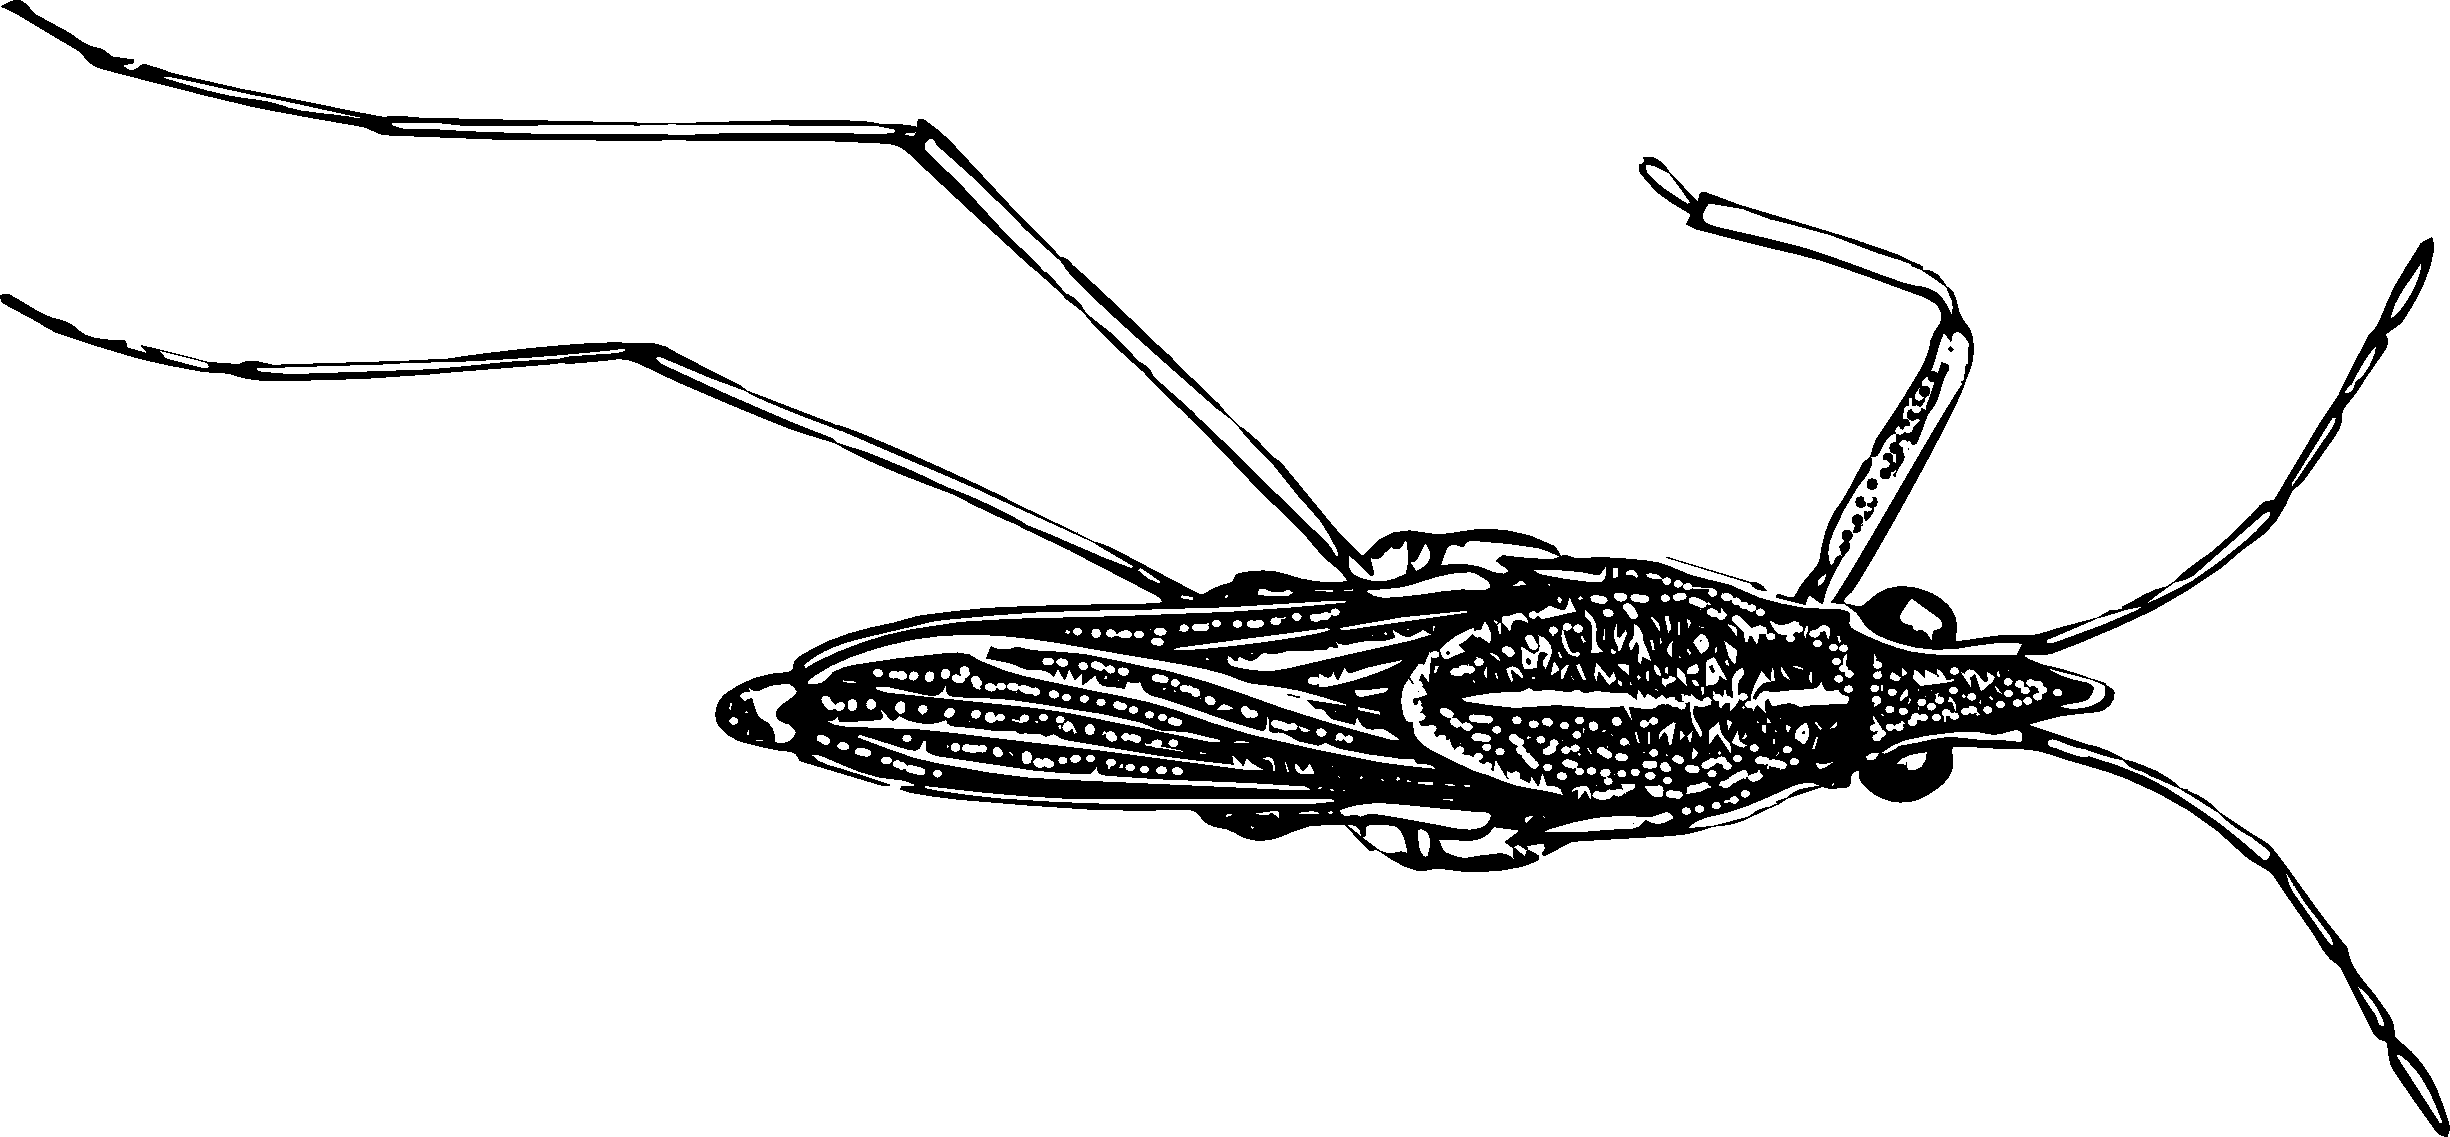
\includegraphics[width=0.5\textwidth]{acercaria/GerridHabitus}
 \caption{Gerridae, dorsal habitus \citep[][Plate 7, Fig. 12]{bhl37902}}
 \label{fig:gerrid1}
\end{figure}

\subsubsection{Veliidae (ripple or riffle bugs)}\index{Veliidae}
\noindent{}\textit{Diagnostic characters:} Body relatively small, 1.6--5.5 mm; antennae longer than head (figure \ref{fig:veliid1}); mid-legs arise midway between fore and hind legs; hind femur shorter than abdomen.\vspace{3mm}

\noindent{}\textit{Natural history:} Almost 1,000 species have been described worldwide, all of which are semiaquatic on still water or in lotic habitats. These insects likewise forage on other invertebrates that fall in the water.\vspace{3mm}

\begin{figure}[ht!]
 \centering
 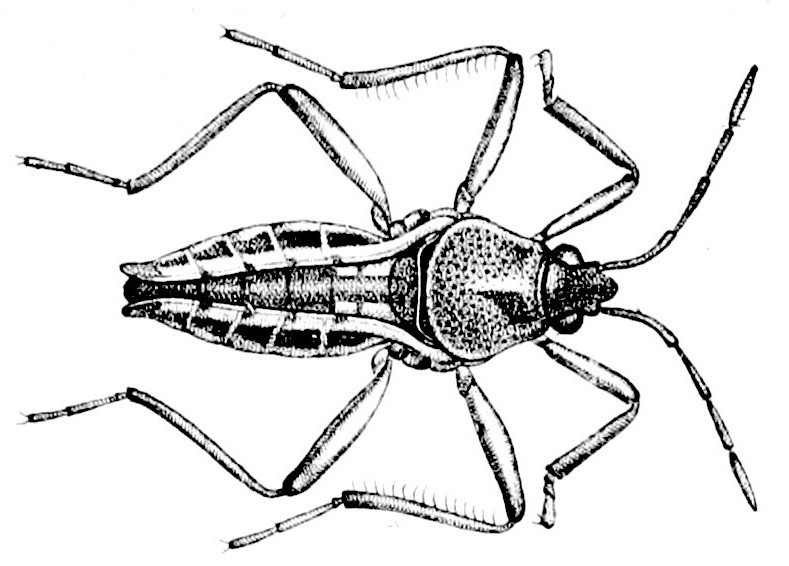
\includegraphics[width=0.4\textwidth]{acercaria/VeliidHabitus}
 \caption{Veliidae, dorsal habitus \citep[][Plate 7, Fig. 11]{bhl37902}}
 \label{fig:veliid1}
\end{figure}

\subsubsection{Leptopodomorpha}\index{Leptopodomorpha}
The two families in this infraorder include species that live as predators, primarily along the edges of water bodies.

\subsubsection{Saldidae (shore bugs)}\index{Saldidae}
\noindent{}\textit{Diagnostic characters:} dorso-ventrally flattened, typically brownish; antenna with 4 antennomeres; labium with 3 sclerites; tarsus with 3 tarsomeres; membrane of fore wing with 4--5 long closed cells (figure \ref{fig:saldids}).\vspace{3mm}

\noindent{}\textit{Natural history:} The only family in Leptopodomorpha that occurs in our area (Northeastern USA). About 350 species are known in the world. They are frequently found near bodies of water (ponds, rivers, etc.), usually on stones or other substrates at the water's edge. They are predators.\vspace{3mm}

\begin{figure}[ht!]
 \centering
 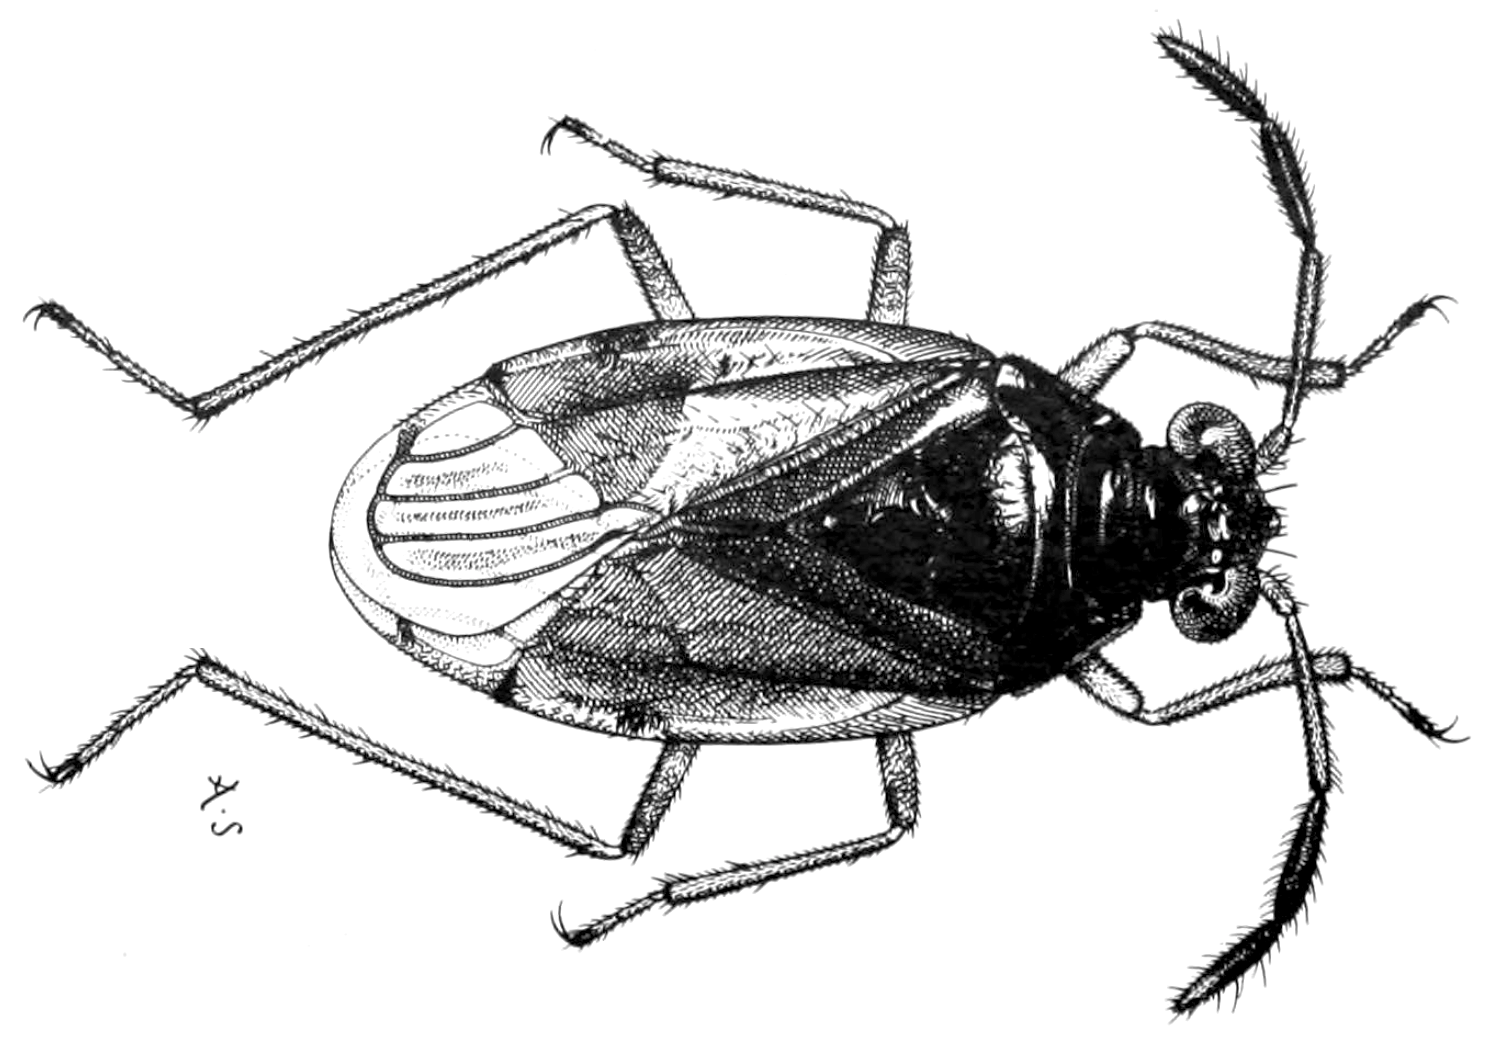
\includegraphics[width=0.5\textwidth]{acercaria/saldidae}
 \caption{Saldidae, dorsal habitus \citep[][Fig. 7:40b]{bhlitem126080aquatic}}
 \label{fig:saldids}
\end{figure}

\subsubsection{Cimicomorpha}\index{Cimicomorpha}
This infraorder is one of the two largest in Heteroptera, with almost 20 families. These species are primarily adapted for feeding as predators or parasites, although two large families, Miridae and Tingidae, live almost exclusively as herbivores.
\subsubsection{Miridae (plant bugs)}\index{Miridae}
\noindent{}\textit{Diagnostic characters:} Antenna with 4 antennomeres; ocelli absent; labium with 4 sclerites; tarsus with 3 tarsomeres; trichobothria present on middle and hind femora; cuneus present (compare to taxon with cuneus absent, like Nabidae); membrane with 2 closed cells (figure \ref{fig:mirid}); wings wide, abdomen at most slightly exposed laterally.\vspace{3mm}

\noindent{}\textit{Natural history:} Worldwide there are \textgreater10,000 described species, and a majority are plant feeders (a few are predators). Instars of many species have a eversible rectums that help these insects gain purchase on foliage.\vspace{3mm}

\begin{figure}[ht!]
 \centering
 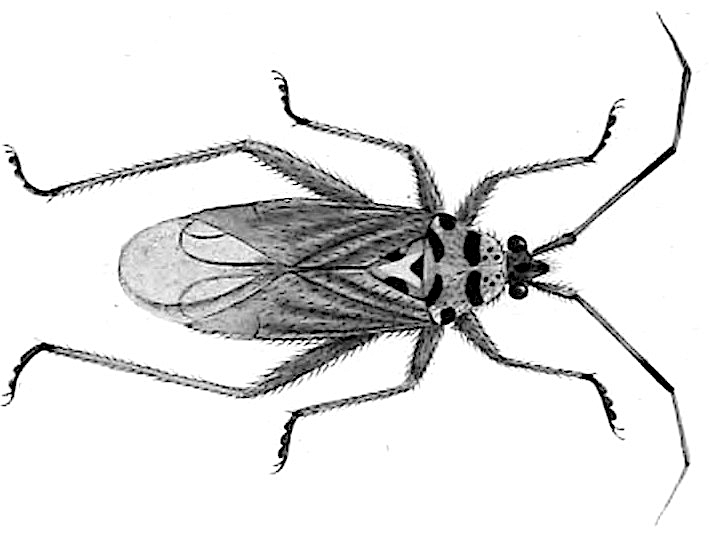
\includegraphics[width=0.5\textwidth]{acercaria/MiridHabitus}
 \caption{Miridae, dorsal habitus \citep[][Plate II, Fig. 1]{bhl132930}}
 \label{fig:mirid}
\end{figure}

\subsubsection{Reduviidae (assassin and ambush bugs)}\index{Reduviidae}
\noindent{}\textit{Diagnostic characters:} Antenna with 4 antennomeres; ocelli present or absent; labium with 3 sclerites; each leg with 1--3 tarsomeres; cuneus absent; fore leg raptorial; prothorax usually with a ventral, longitudinal scrobe accommodating the long and robust mouthparts; wings wide, abdomen at most slightly exposed laterally.\vspace{3mm}

\noindent{}\textit{Natural history:} As their common name implies these insects are mostly predators; some, however, have become parasites (including important species that vector human diseases, like trypanosomiasis). About 7,000 species are known worldwide, and they vary considerably in their habitus and size.\vspace{3mm}

\begin{figure}[ht!]
 \centering
 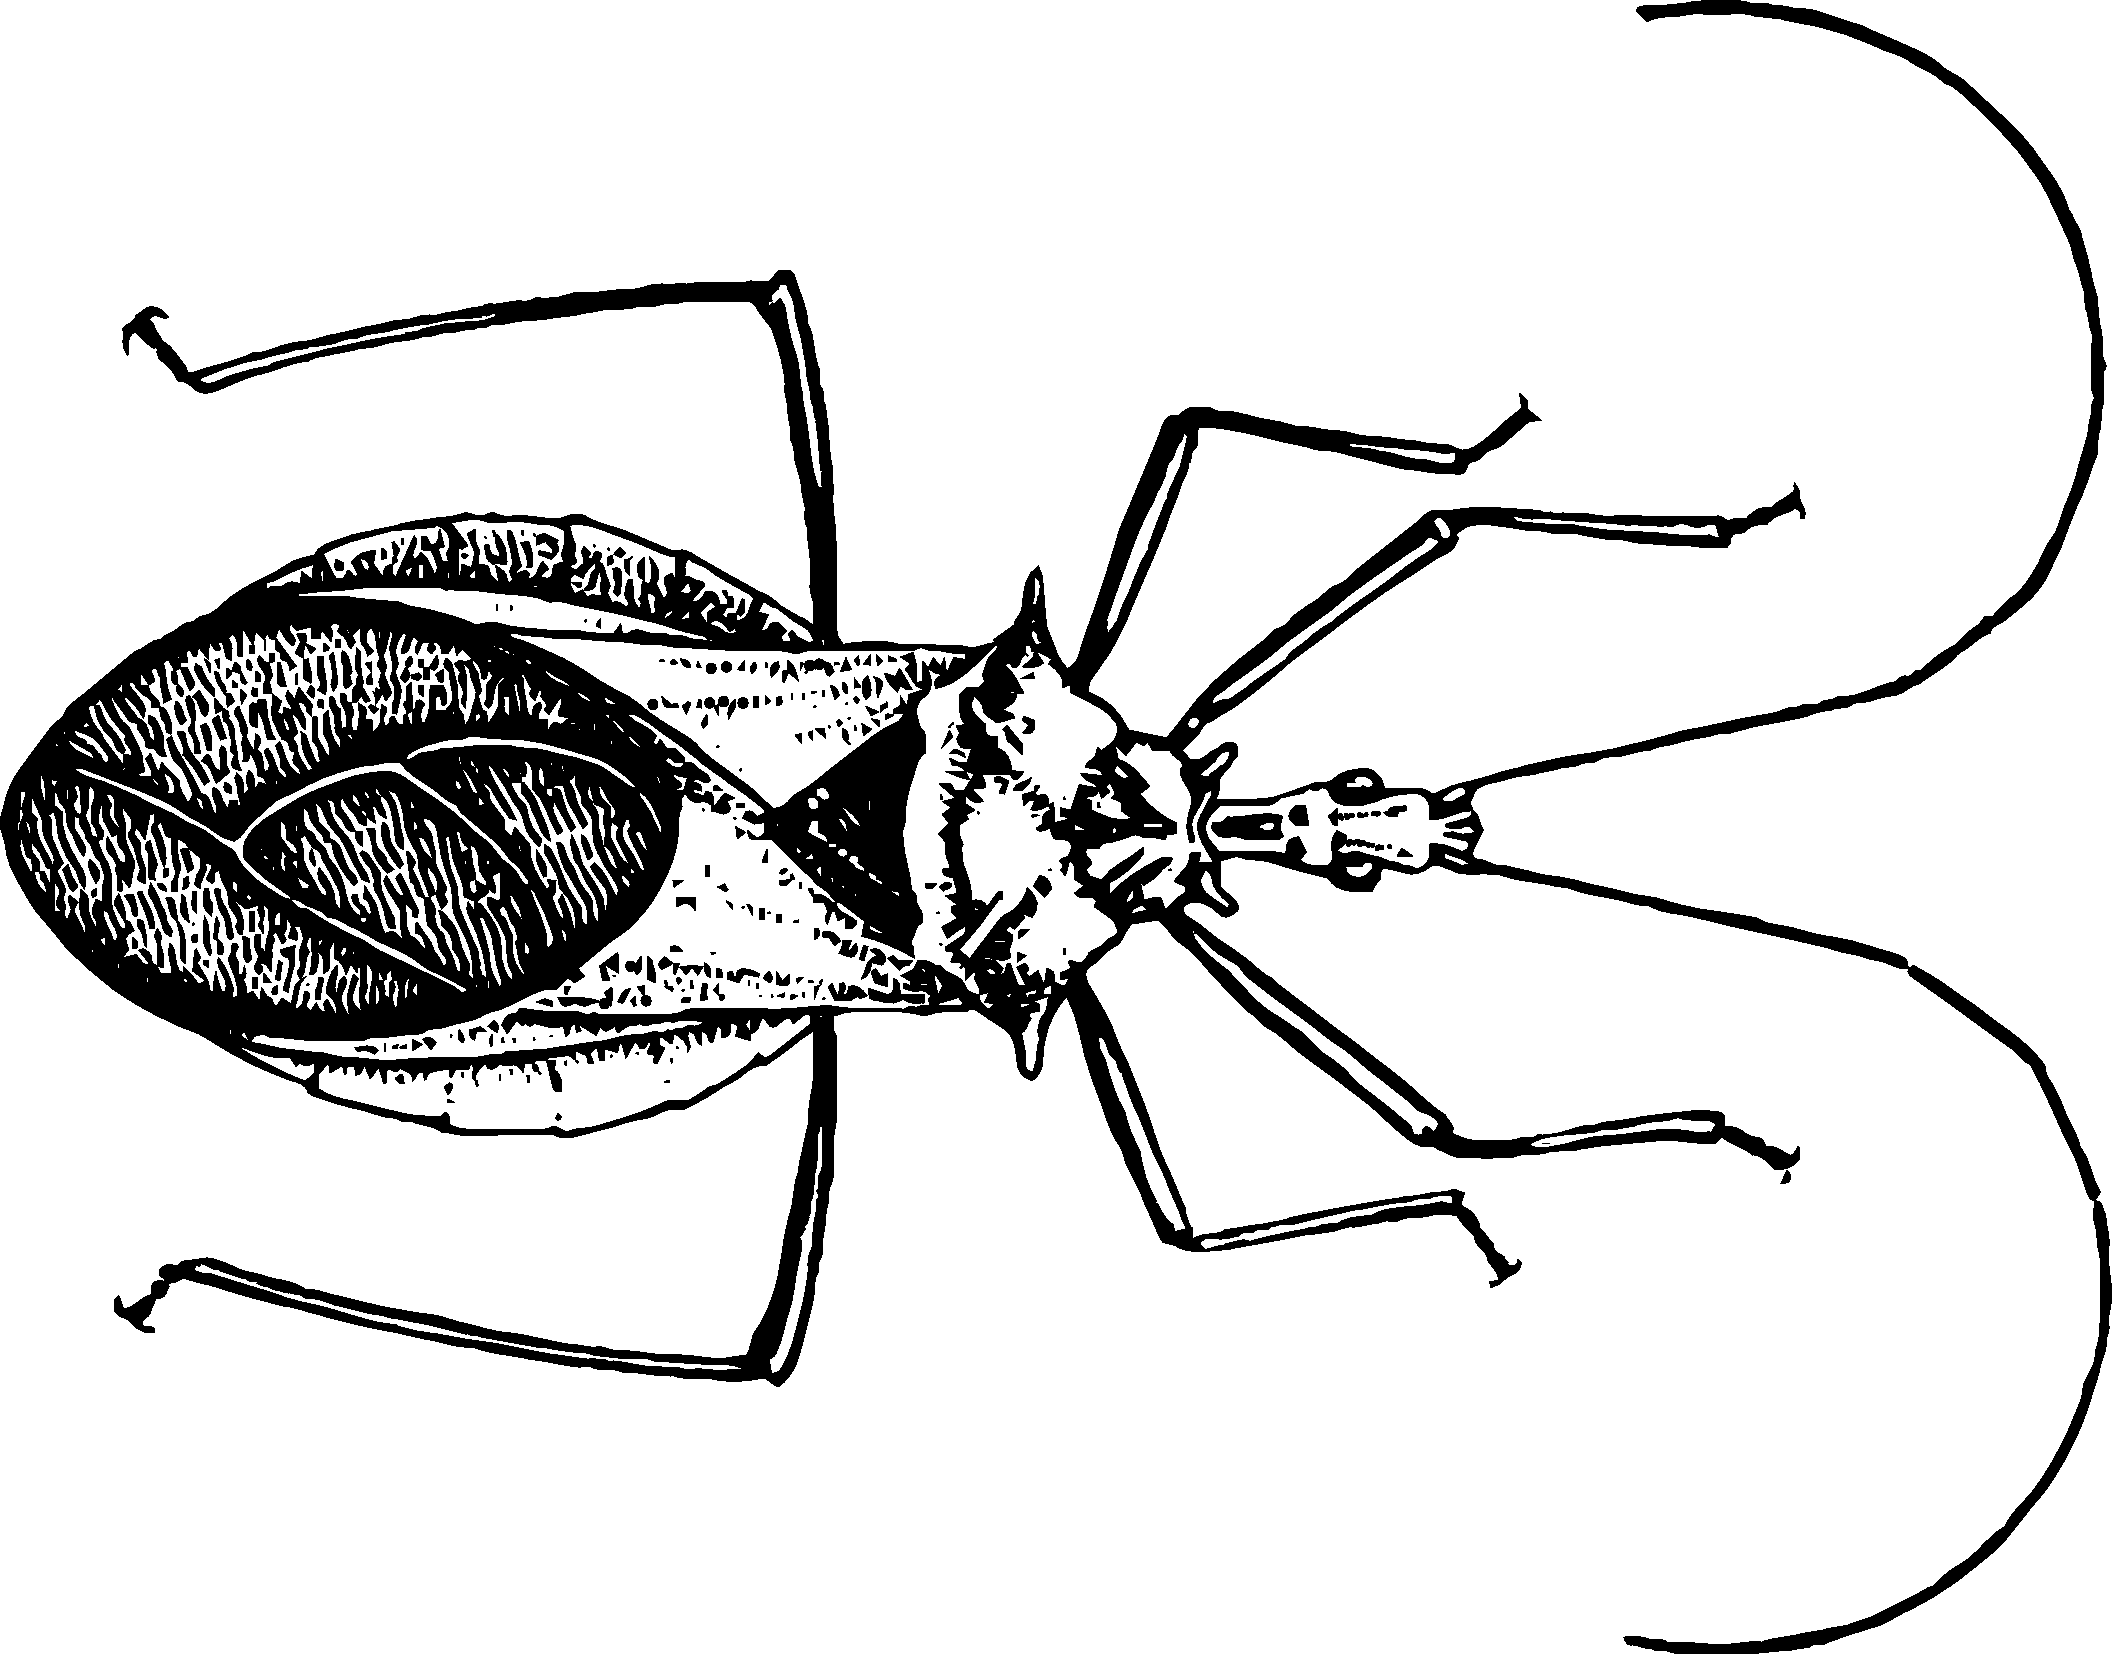
\includegraphics[width=0.5\textwidth]{acercaria/ReduviidHabitus}
 \caption{Reduviidae habitus \citep[redrawn from][Plate XXXII, Fig. 12]{bhlitem82061AustrInsect}}
 \label{fig:reduviid1}
\end{figure}

\subsubsection{Anthocoridae (minute pirate bugs)}\index{Anthocoridae}
\noindent{}\textit{Diagnostic characters:} Antenna with 4 antennomeres; labium with 3 sclerites; ocelli present; tarsus with 2--3 tarsomeres; front legs not raptorial; cuneus present; membrane with no closed cells, with one or two usually rudimentary longitudinal veins; wings wide, abdomen at most slightly exposed laterally (figure \ref{fig:anthocorid1}).\vspace{3mm}

\noindent{}\textit{Natural history:} Approximately 600 species are known worldwide, all of which are predators and (often) facultative parasites. This family is likely sister to Cimicidae, and both families exhibit ``traumatic insemination''.\vspace{3mm}

\begin{figure}[ht!]
 \centering
 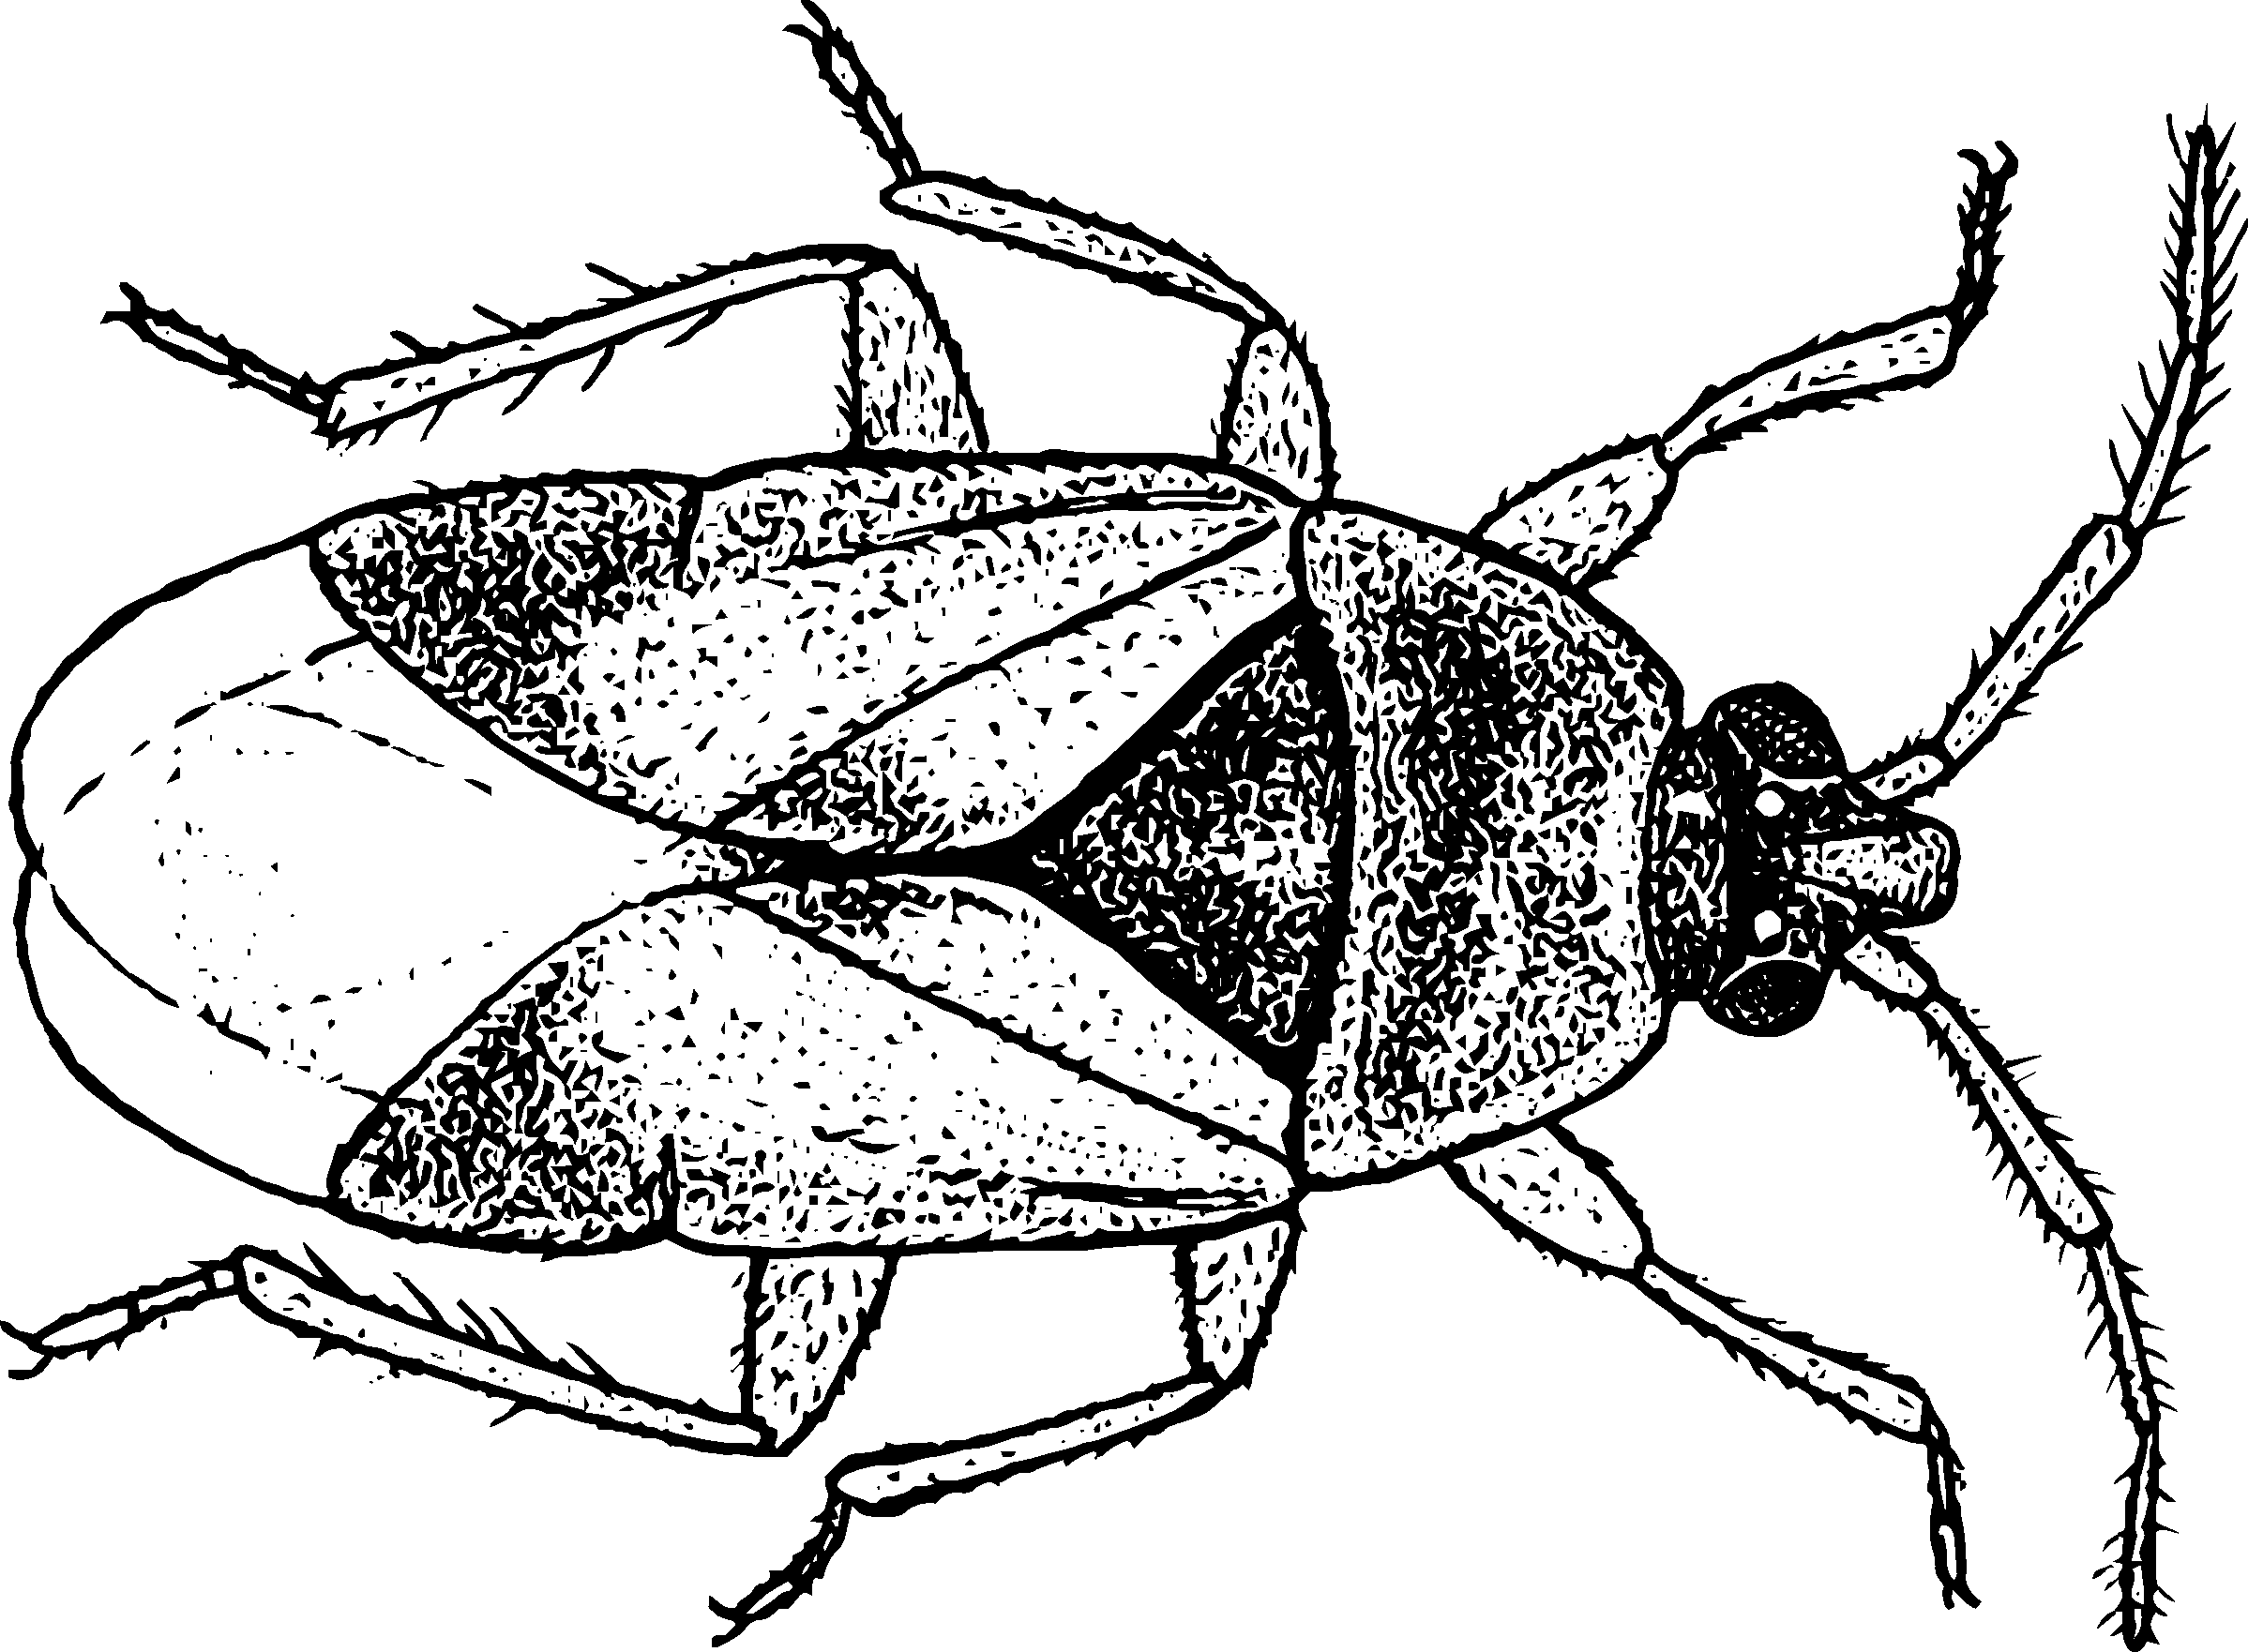
\includegraphics[width=0.4\textwidth]{acercaria/anthocorid}
 \caption{Habitus \citep[redrawn from][Fig. 15K]{prins1984morphological}}
 \label{fig:anthocorid1}
\end{figure}

\subsubsection{Cimicidae (bed bugs, bat bugs)}\index{Cimicidae}
\noindent{}\textit{Diagnostic characters:} Antenna with 4 antennomeres; labium with 3 sclerites; ocelli absent; number of tarsomeres: 2--3; wings absent.\vspace{3mm}

\noindent{}\textit{Natural history:} All 110 known species are parasites of birds and mammals (especially bats).\vspace{3mm}

\begin{theo}
{}In the previous two families can you see structures you think might facilitate traumatic insemination? How would such a mating strategy evolve? Note that some species in other heteropteran families, including Nabidae and Miridae, have also evolved this mating strategy.
\end{theo}

\begin{figure}[ht!]
 \centering
 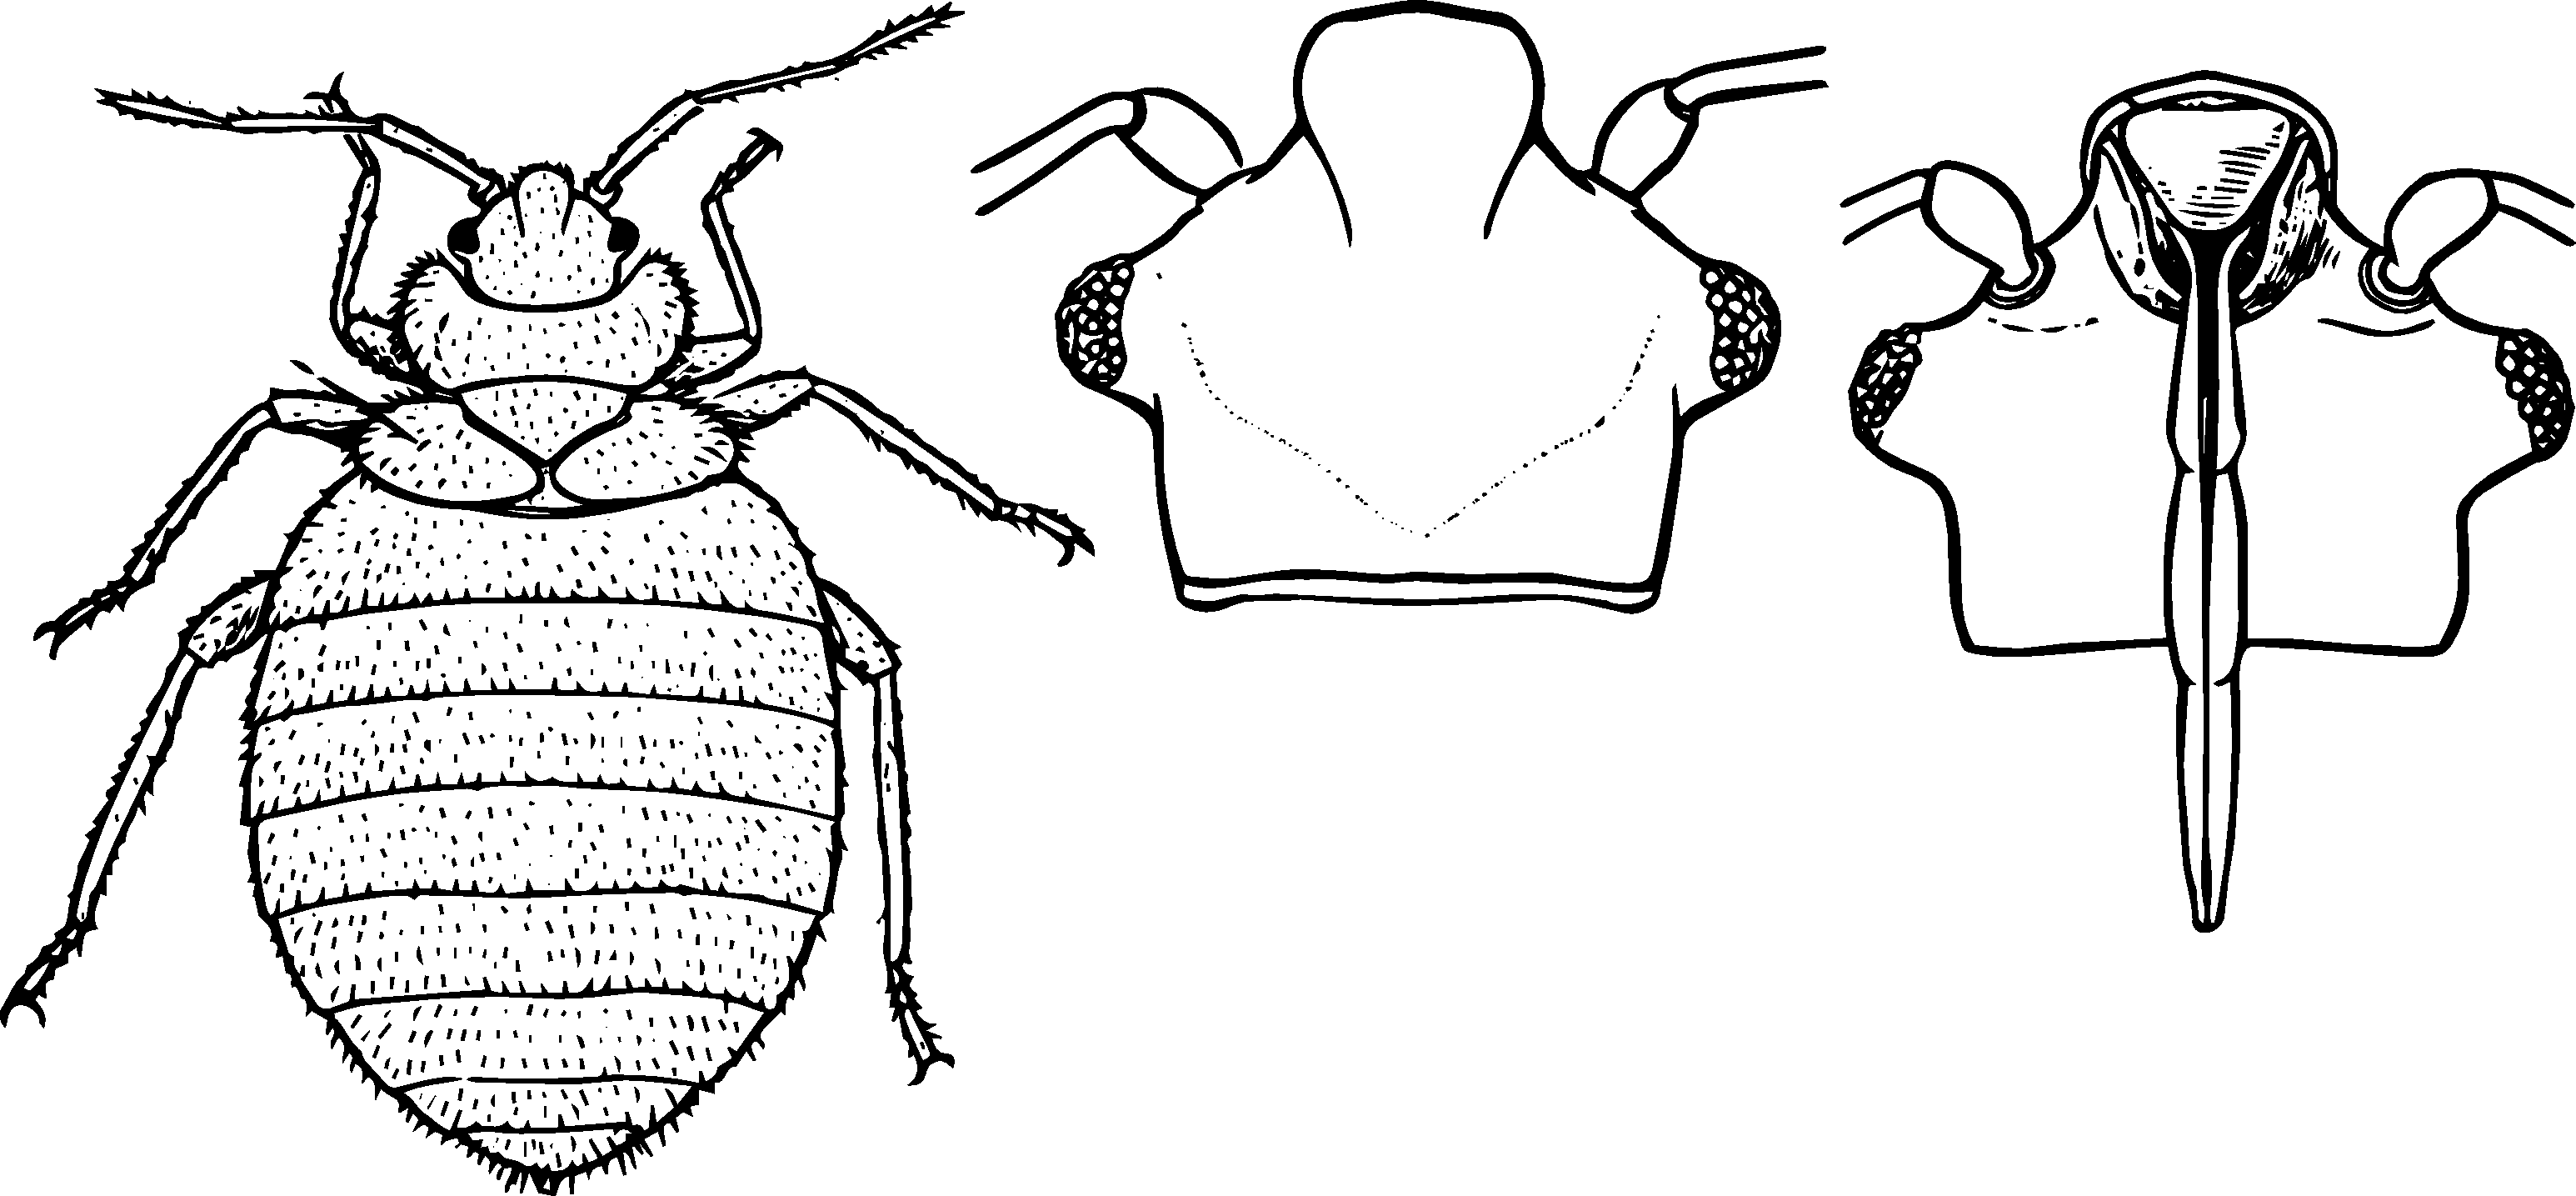
\includegraphics[width=0.7\textwidth]{acercaria/cimicids}
 \caption{Cimicidae habitus and head (dorsal, ventral) \citep[Modified from Fig. 38A in][]{snodgrass1944feeding}}
 \label{fig:cimicid1}
\end{figure}

\subsubsection{Tingidae (lace bugs)}\index{Tingidae}
\noindent{}\textit{Diagnostic characters:} body and wings with reticulate ``lace-like'' sculpture (figure \ref{fig:tingid1}); antenna with 4 antennomeres; ocelli present; labium with 4 sclerites;  each leg with 1--2 tarsomeres; cuneus absent; membrane venation obscured by reticulate sculpture; pronotum extends posteriorly obscuring mesoscutellum.\vspace{3mm}

\noindent{}\textit{Natural history:} More than 2,000 species are known worldwide, all of which are relatively small (2--10 mm). They are herbivores, mostly feeding on the underside of leaves. many species exhibit parental care.\vspace{3mm}

\begin{theo}
{}What do you think is the function of the elaborate integumental sculpturing of these bugs? What selection pressure would maintain such a structure?
\end{theo}

\begin{figure}[ht!]
 \centering
 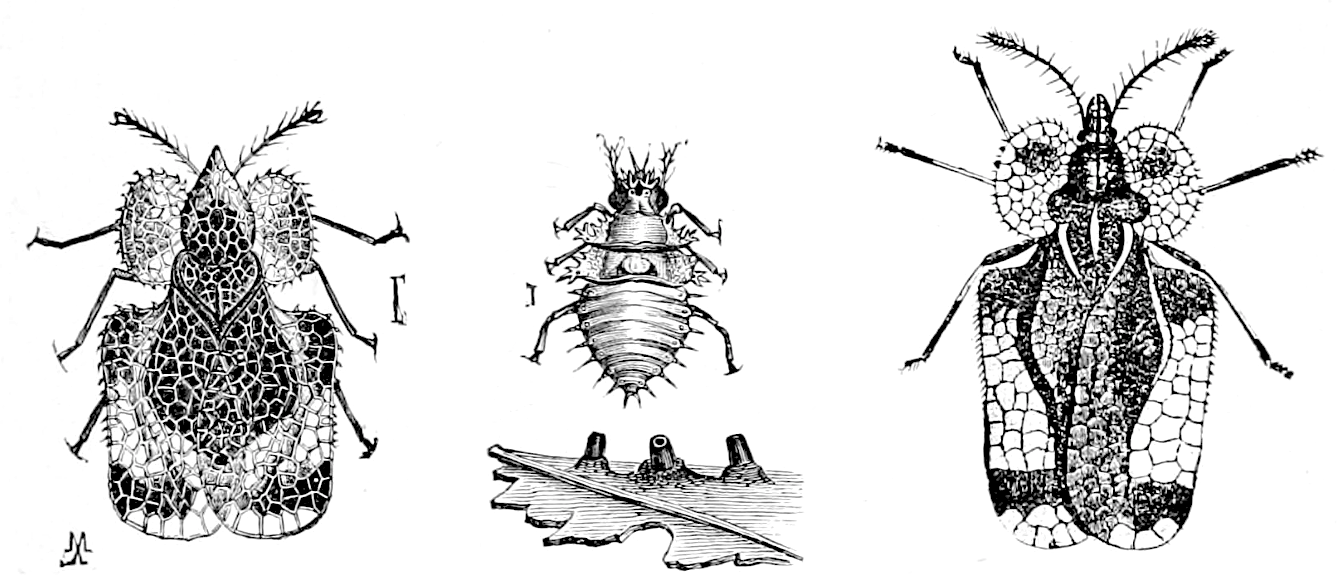
\includegraphics[width=0.7\textwidth]{acercaria/tingids}
 \caption{Tingidae \citep[][Fig. 38]{bhlitem45622}}
 \label{fig:tingid1}
\end{figure}

\subsubsection{Nabidae (damsel bugs)}\index{Nabidae}%need to sight ID?
\noindent{}\textit{Diagnostic characters:} Antenna with 4 antennomeres; labium with 4 sclerites; ocelli present; each leg with 2--3 tarsomeres; fore leg raptorial; cuneus absent; membrane with numerous closed cells or absent; wings wide, abdomen at most slightly exposed laterally.\vspace{3mm}

\noindent{}\textit{Natural history:} About 400 species have been described worldwide. All are predators of other insects, and some species have been cultivated for biocontrol of many pestiferous insects (lepidopteran larvae and eggs especially, but also leafhopper nymphs).\vspace{3mm}

\begin{figure}[ht!]
 \centering
    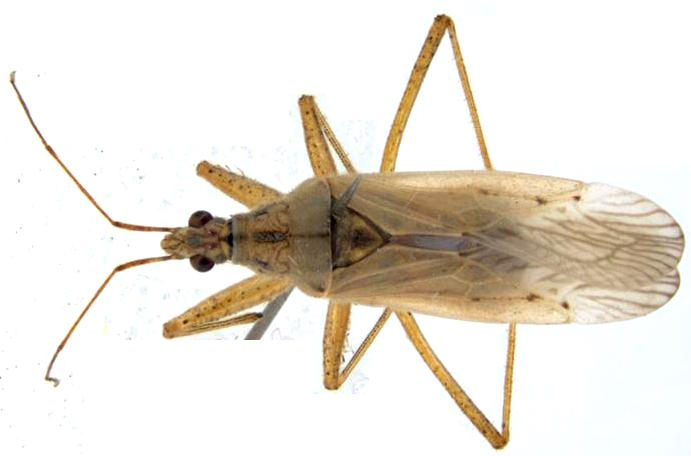
\includegraphics[width=0.5\textwidth]{acercaria/NabidHabitus}
 \caption{Nabidae, dorsal habitus. Illustration (CC BY 4.0) Des Helmore / Manaaki Whenua – Landcare Research. Accessed from Wikimedia Commons}
 \label{fig:nabid1}
\end{figure}

\subsubsection{Pentatomomorpha}\index{Pentatomomorpha}
This infraorder includes more than 40 families is is the most diverse in Heteroptera.
\subsubsection{Berytidae (stilt bugs)}\index{Berytidae}
\noindent{}\textit{Diagnostic characters:} antenna with 4 antennomeres; apical antennomere spindle-shaped; labium with 4 sclerites; each leg with 3 tarsomeres; fore leg not raptorial; cuneus absent; membrane with no closed cells (usually with 5 longitudinal veins); wings wide, abdomen at most slightly exposed laterally.\vspace{3mm}

\noindent{}\textit{Natural history:} About 170 species are known worldwide, most of which are herbivores.\vspace{3mm}

\begin{figure}[ht!]
 \centering
 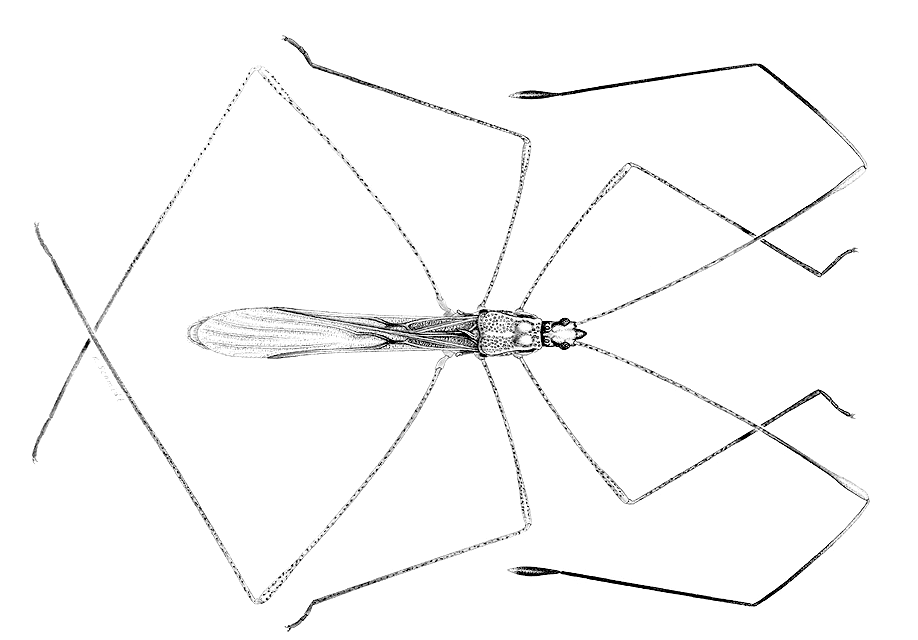
\includegraphics[width=0.55\textwidth]{acercaria/BerytidHabitus}
 \caption{Berytidae, dorsal habitus. Illustration (CC0) by Kathleen Schmidt USDA-ARS}
 \label{fig:berytid1}
\end{figure}

\subsubsection{Lygaeidae (seed bugs)}\index{Lygaeidae}%mention other families??
\noindent{}\textit{Diagnostic characters:} Head narrower than pronotum; antenna with 4 antennomeres; labium with 4 sclerites; each leg with 3 tarsomeres; fore leg not raptorial; cuneus absent; membrane with no closed cells; wings wide, abdomen at most slightly exposed laterally; abdominal spiracles 5--7 located dorsally.\vspace{3mm}

\noindent{}\textit{Natural history:} About 1,000 species are known, the vast majority of which are herbivores that specialize on seeds. The milkweed bug, \textit{Oncopeltus fasciatus} (Dallas, 1852) (figure \ref{fig:oncopeltus}) frequently serves as a model for ecological research and evolutionary developmental (evo-devo) biology. Several species are considered pests.\vspace{3mm}

\begin{figure}[ht!]
 \centering
 \begin{subfigure}[ht!]{0.45\textwidth}
  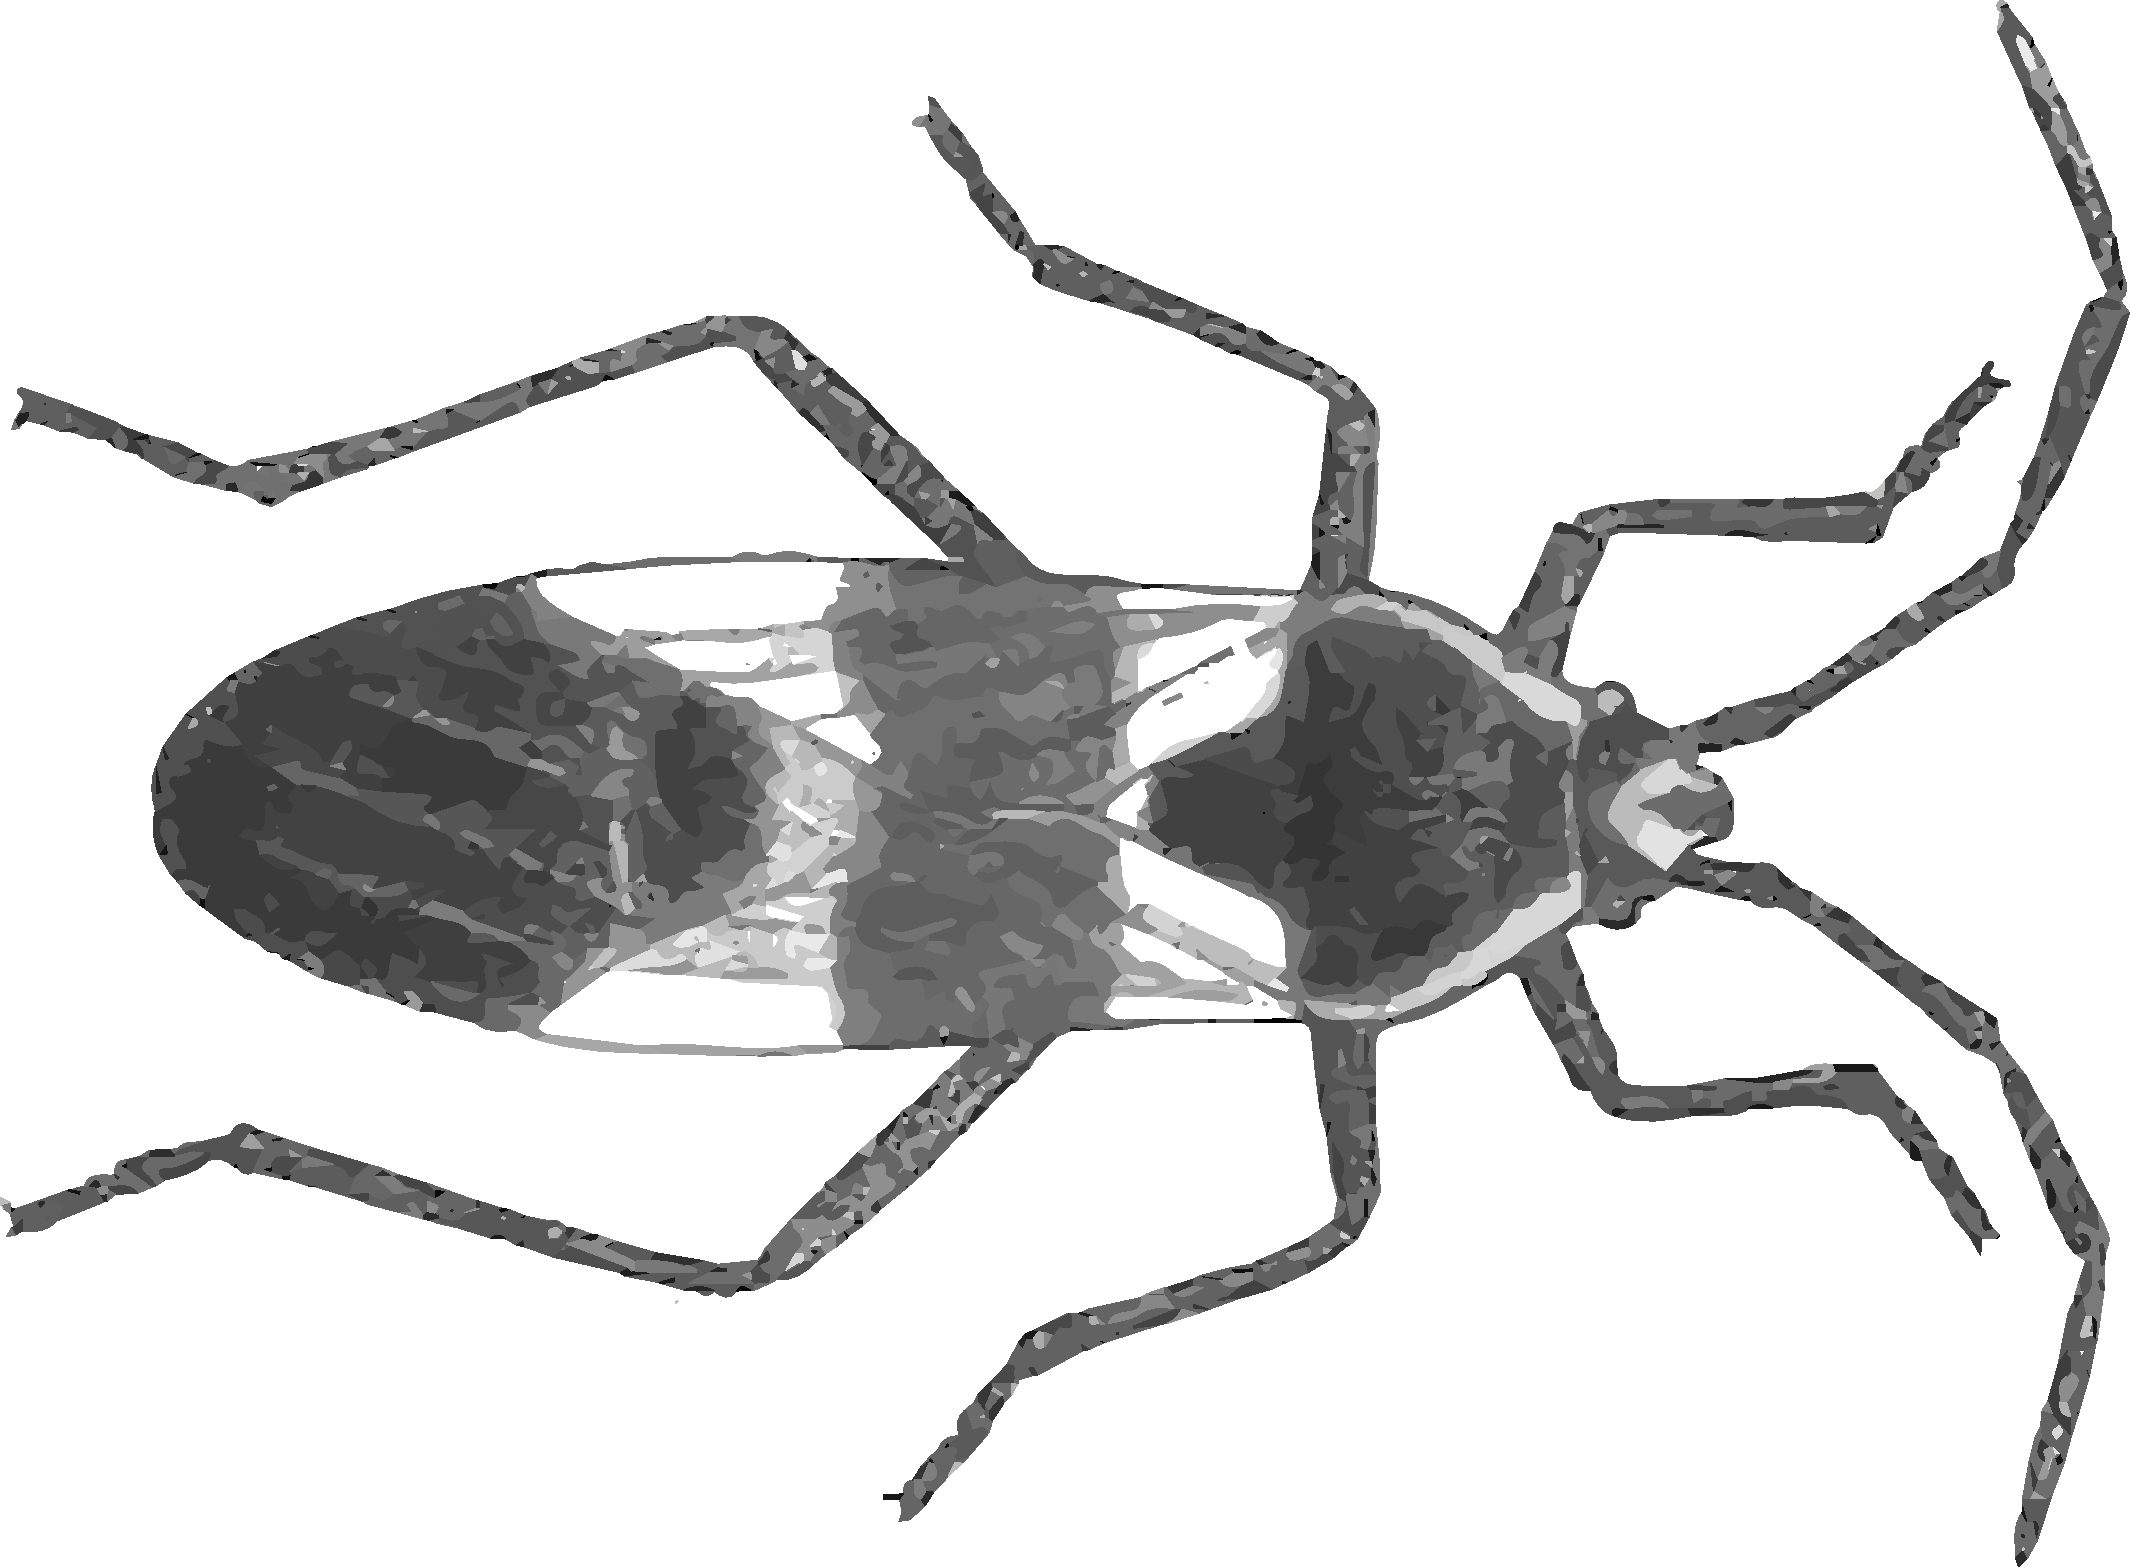
\includegraphics[width=\textwidth]{acercaria/LygaeidHabitus}
  \caption{}
  \label{fig:oncopeltus}
 \end{subfigure}
 \hfill
 \begin{subfigure}[ht!]{0.45\textwidth}
  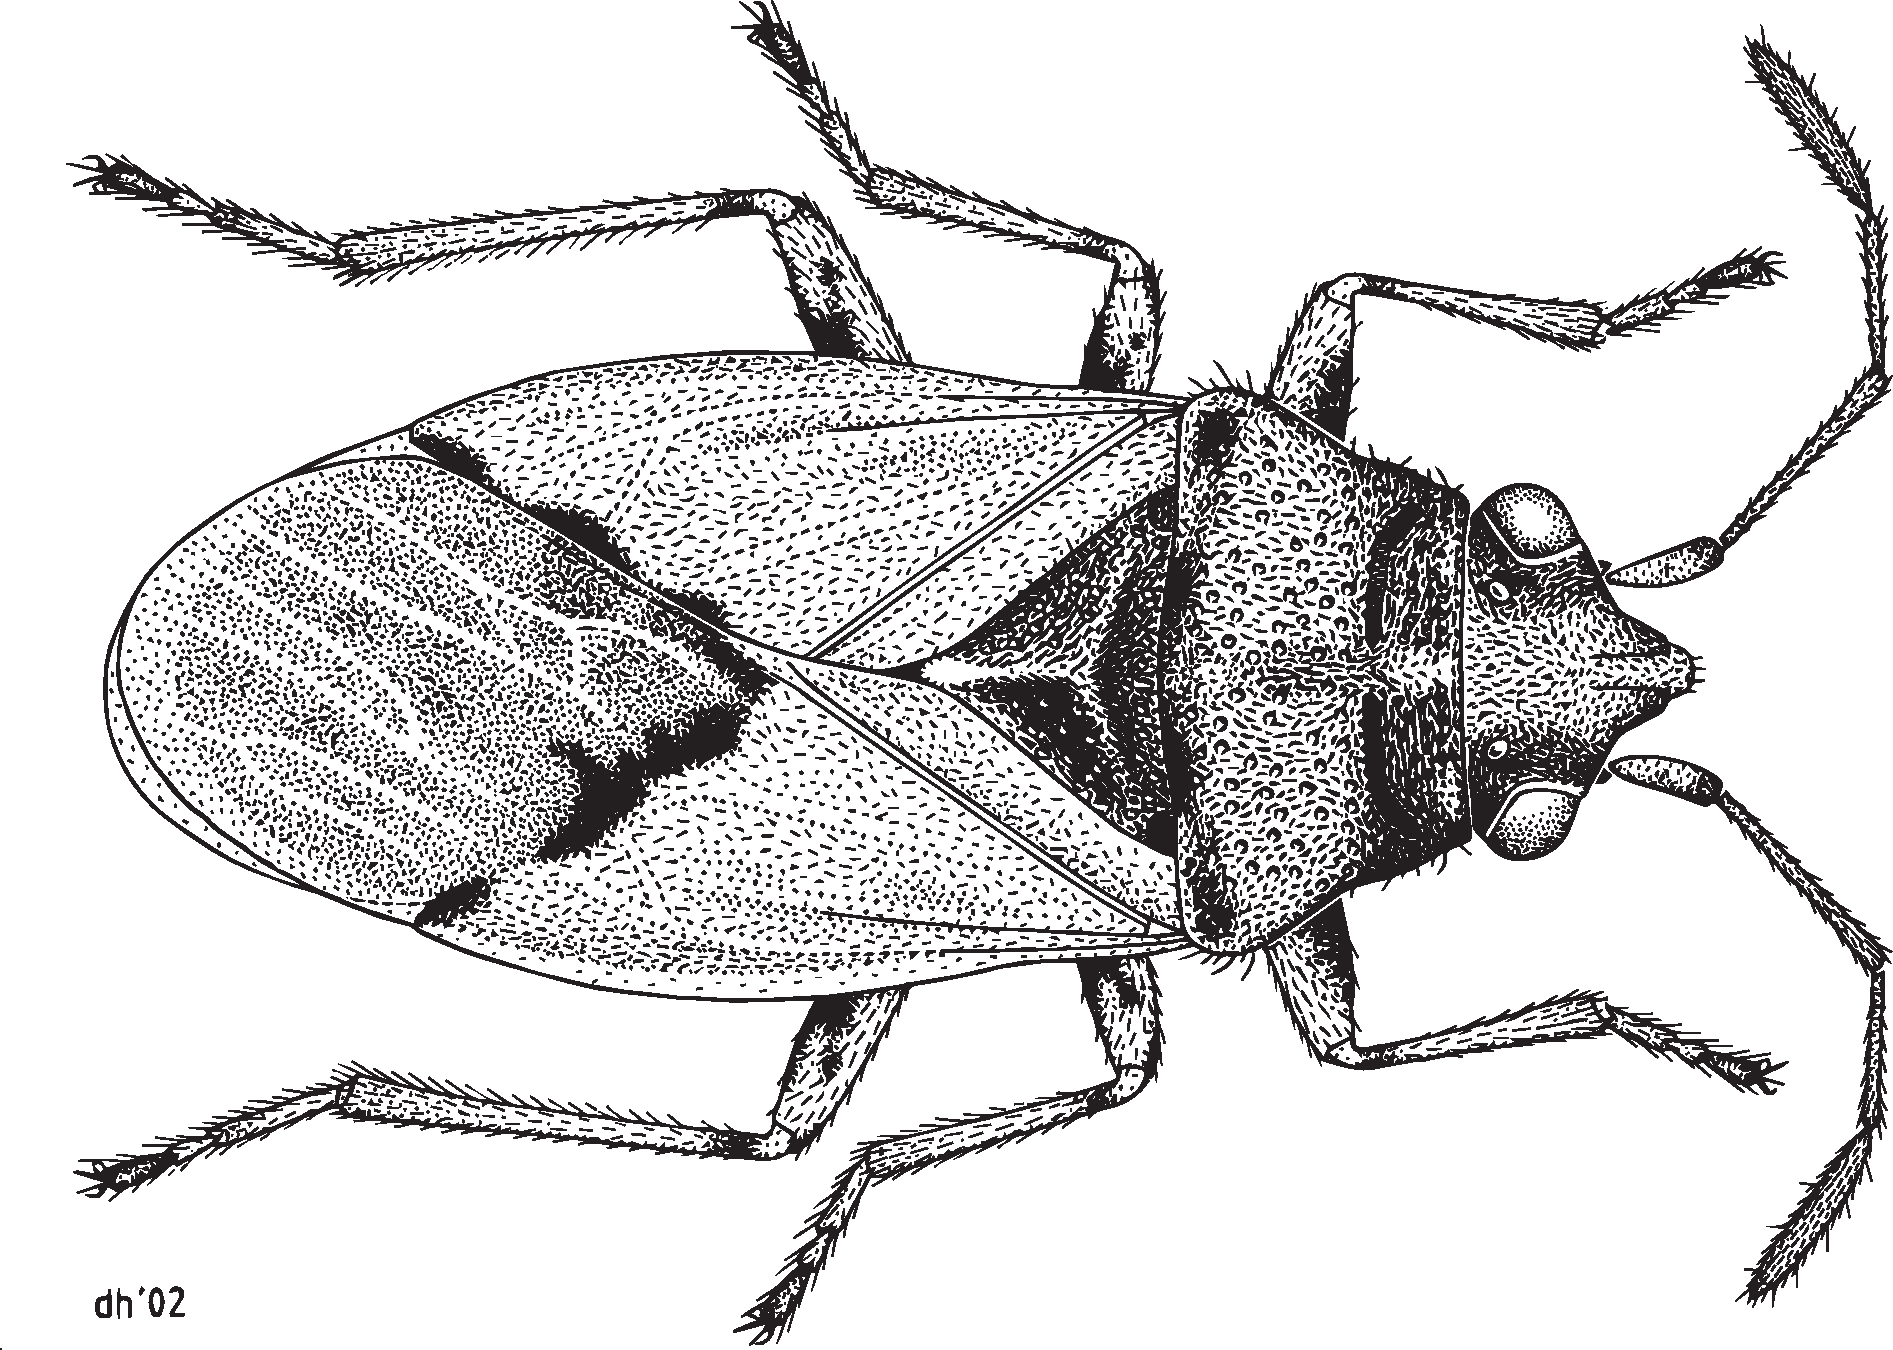
\includegraphics[width=\textwidth]{acercaria/Lygaeidae}
  \caption{}
  \label{fig:lygaeid}
 \end{subfigure}
 \caption{Lygaeidae. \textbf{(a)} Habitus \citep[redrawn from][Plate 16, Fig. 23]{bhl14630}; \textbf{(b)} habitus (modified from illustration by Des Helmore, Manaaki Whenua – Landcare Research}\label{fig:lygaeid1}
\end{figure}

\subsubsection{Geocoridae (big-eyed bugs)}\index{Geocoridae}
\noindent{}\textit{Diagnostic characters:} Head wider than pronotum (figure \ref{fig:geocorid1}); antenna with 4 antennomeres; labium with 4 sclerites; ocelli present; each leg with 3 tarsomeres; fore leg not raptorial; cuneus absent; wings wide, abdomen at most slightly exposed laterally; abdominal spiracles 5--7 ventrally located.\vspace{3mm}

\noindent{}\textit{Natural history:} Approximately 275 species are known worldwide, and most are 3--5 mm in length. They are predators of other insects and have been used in a biocontrol context.\vspace{3mm}

\begin{figure}[ht!]
 \centering
 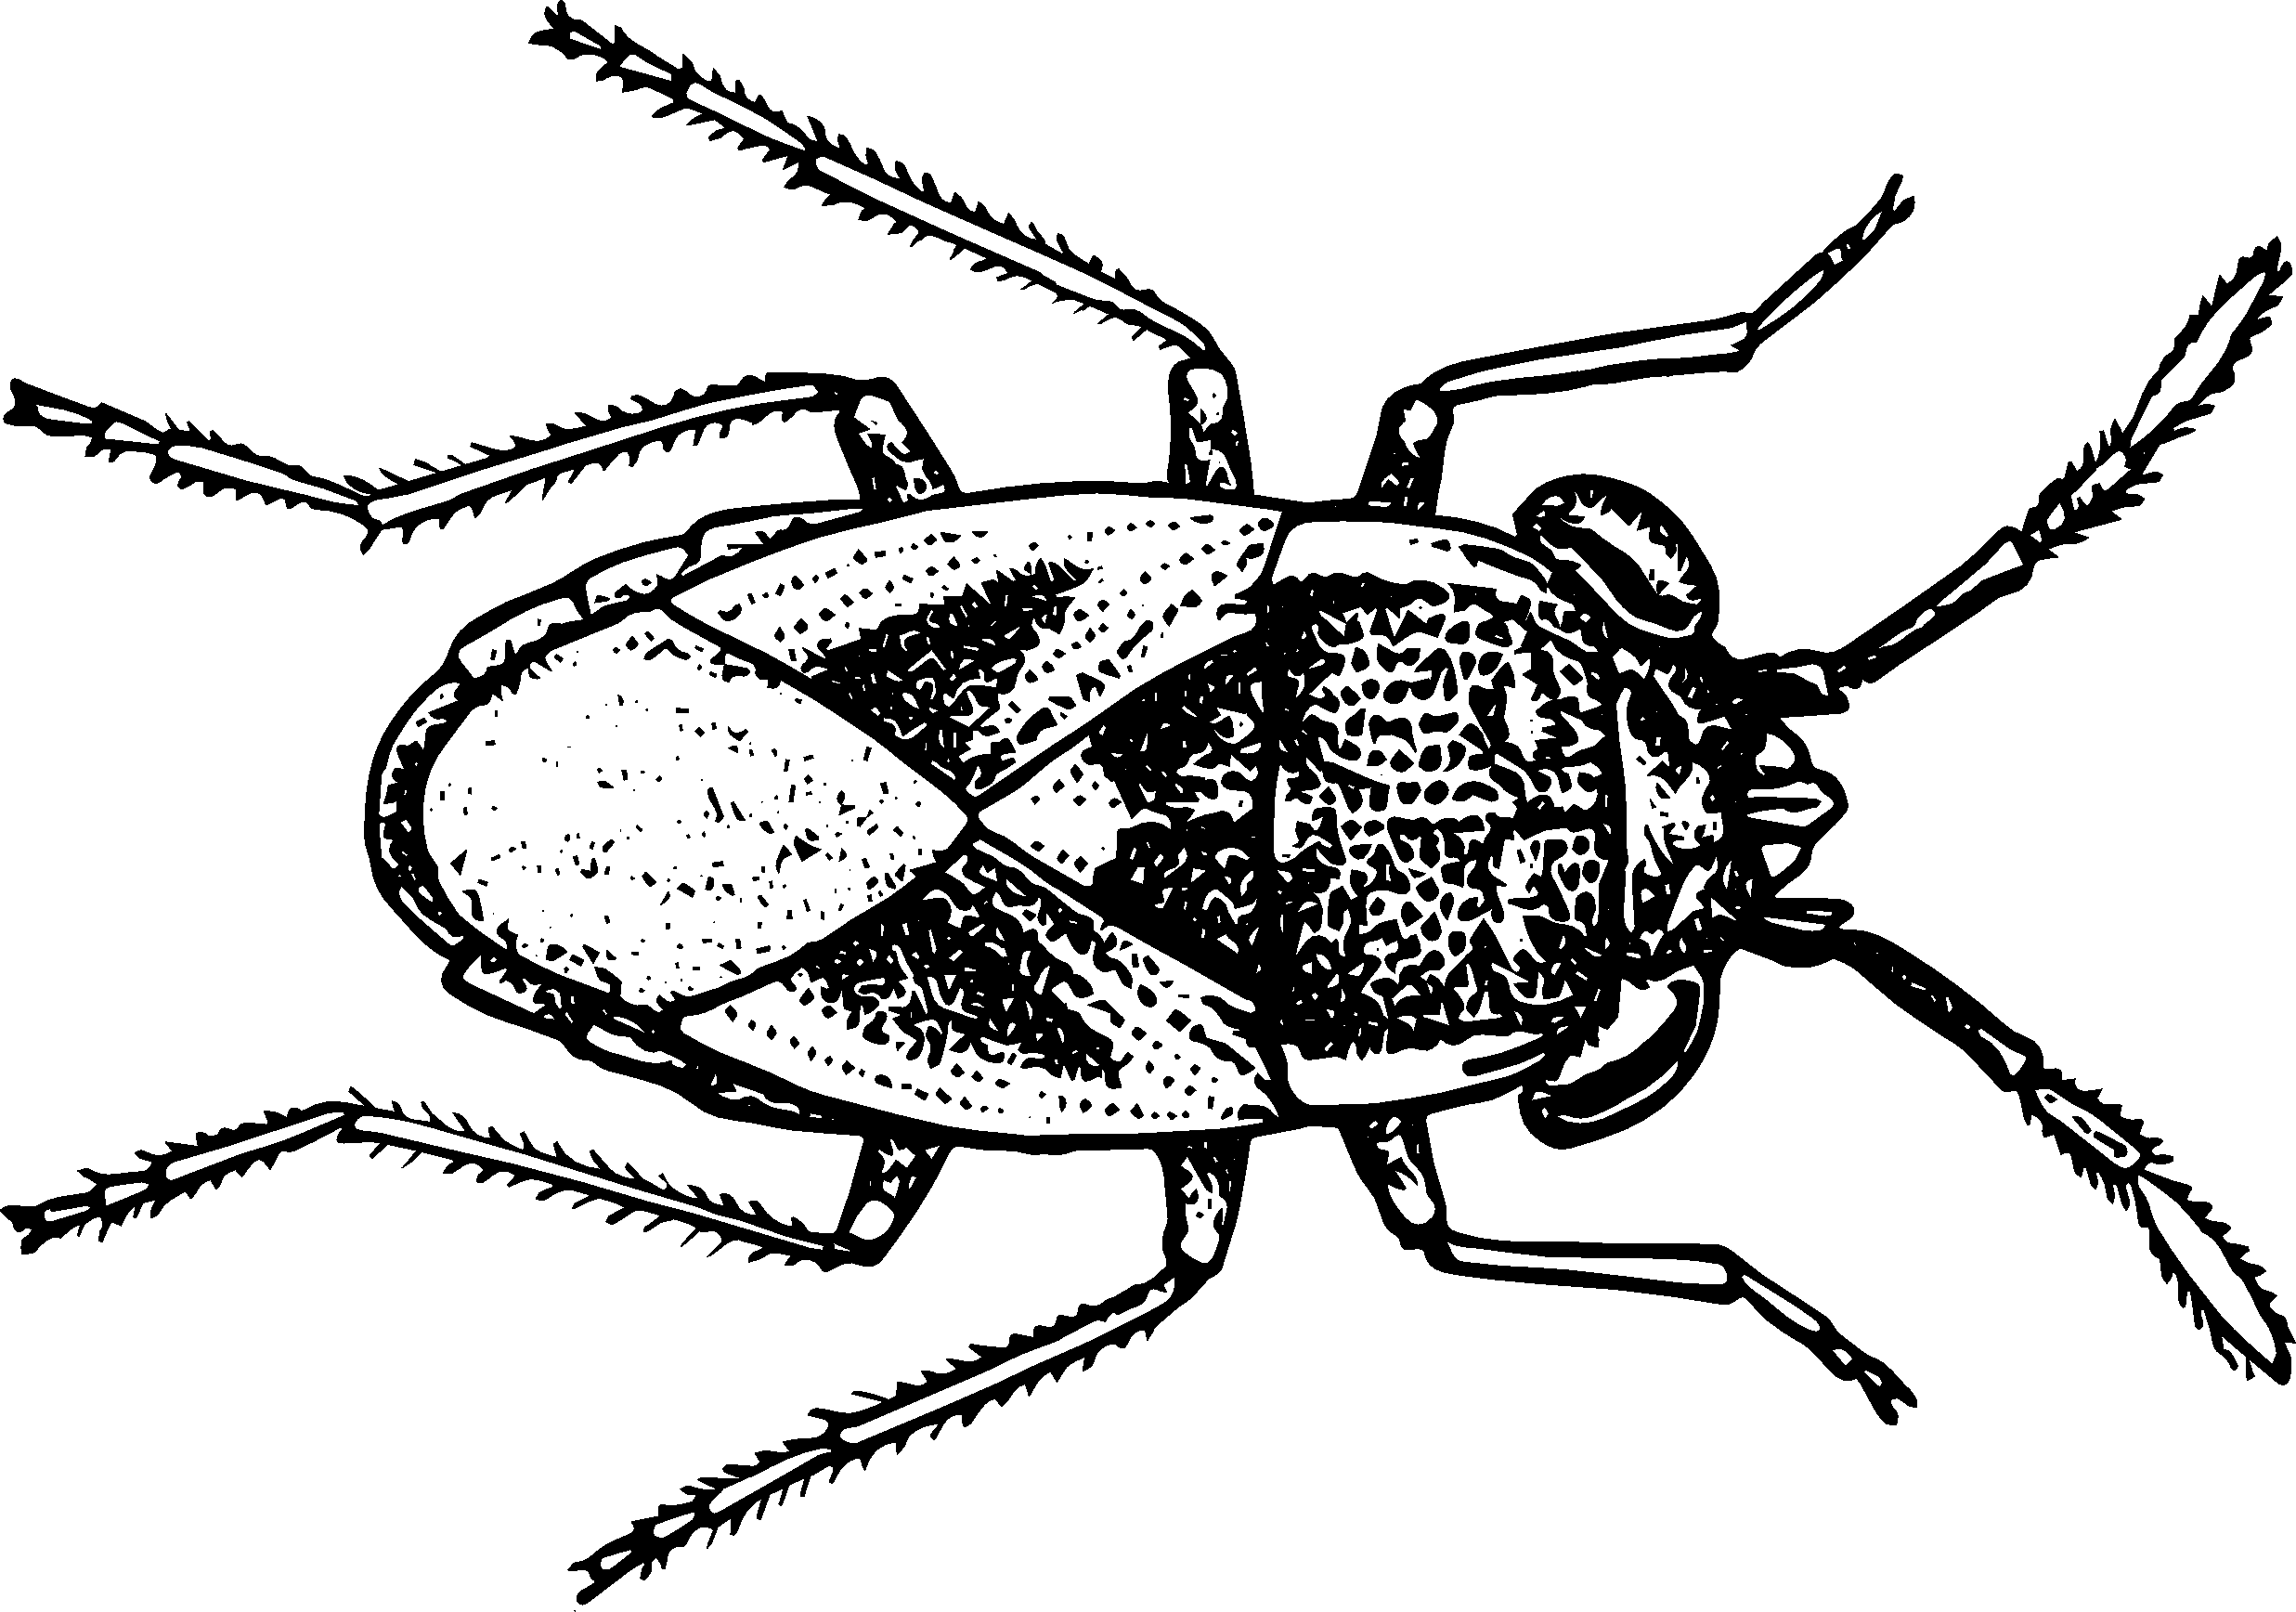
\includegraphics[width=0.5\textwidth]{acercaria/geocorid}
 \caption{Geocoridae, dorsal habitus \citep[modified from][Fig. 11]{distant1904fauna}}
 \label{fig:geocorid1}
\end{figure}

\begin{theo}
{}Take a look at the head shape in Geocoridae, and it compare to Lygaeidae; they used to be classified as one family. Do you see any differences that relate to their diets?
\end{theo}

\subsubsection{Coreidae (leaf-footed bugs)}\index{Coreidae}
\noindent{}\textit{Diagnostic characters:} Head narrower and shorter than pronotum; antenna with 4 antennomeres; labium with 4 labial sclerites; ocelli present; each leg with 3 tarsomeres; cuneus absent; wings wide, abdomen at most slightly exposed laterally; hind tibia usually widened, leaf-shaped.\vspace{3mm}

\noindent{}\textit{Natural history:} Almost 2,000 species have been described worldwide, and they tend to be large-bodied bugs (7--45 mm long). Evidence suggest they are all herbivores, and some species (\textit{e.g.}, \textit{Anasa tristis} (De Geer, 1773)) are major pests.\vspace{3mm}

\begin{figure}[ht!]
 \centering
 \begin{subfigure}[ht!]{0.35\textwidth}
  \reflectbox{%
  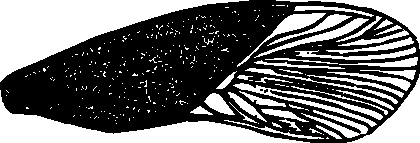
\includegraphics[width=\textwidth]{acercaria/CoreidaeWing}}
  \caption{}
  \label{fig:coreid2}
 \end{subfigure}
 \hfill
  \begin{subfigure}[ht!]{0.45\textwidth}
  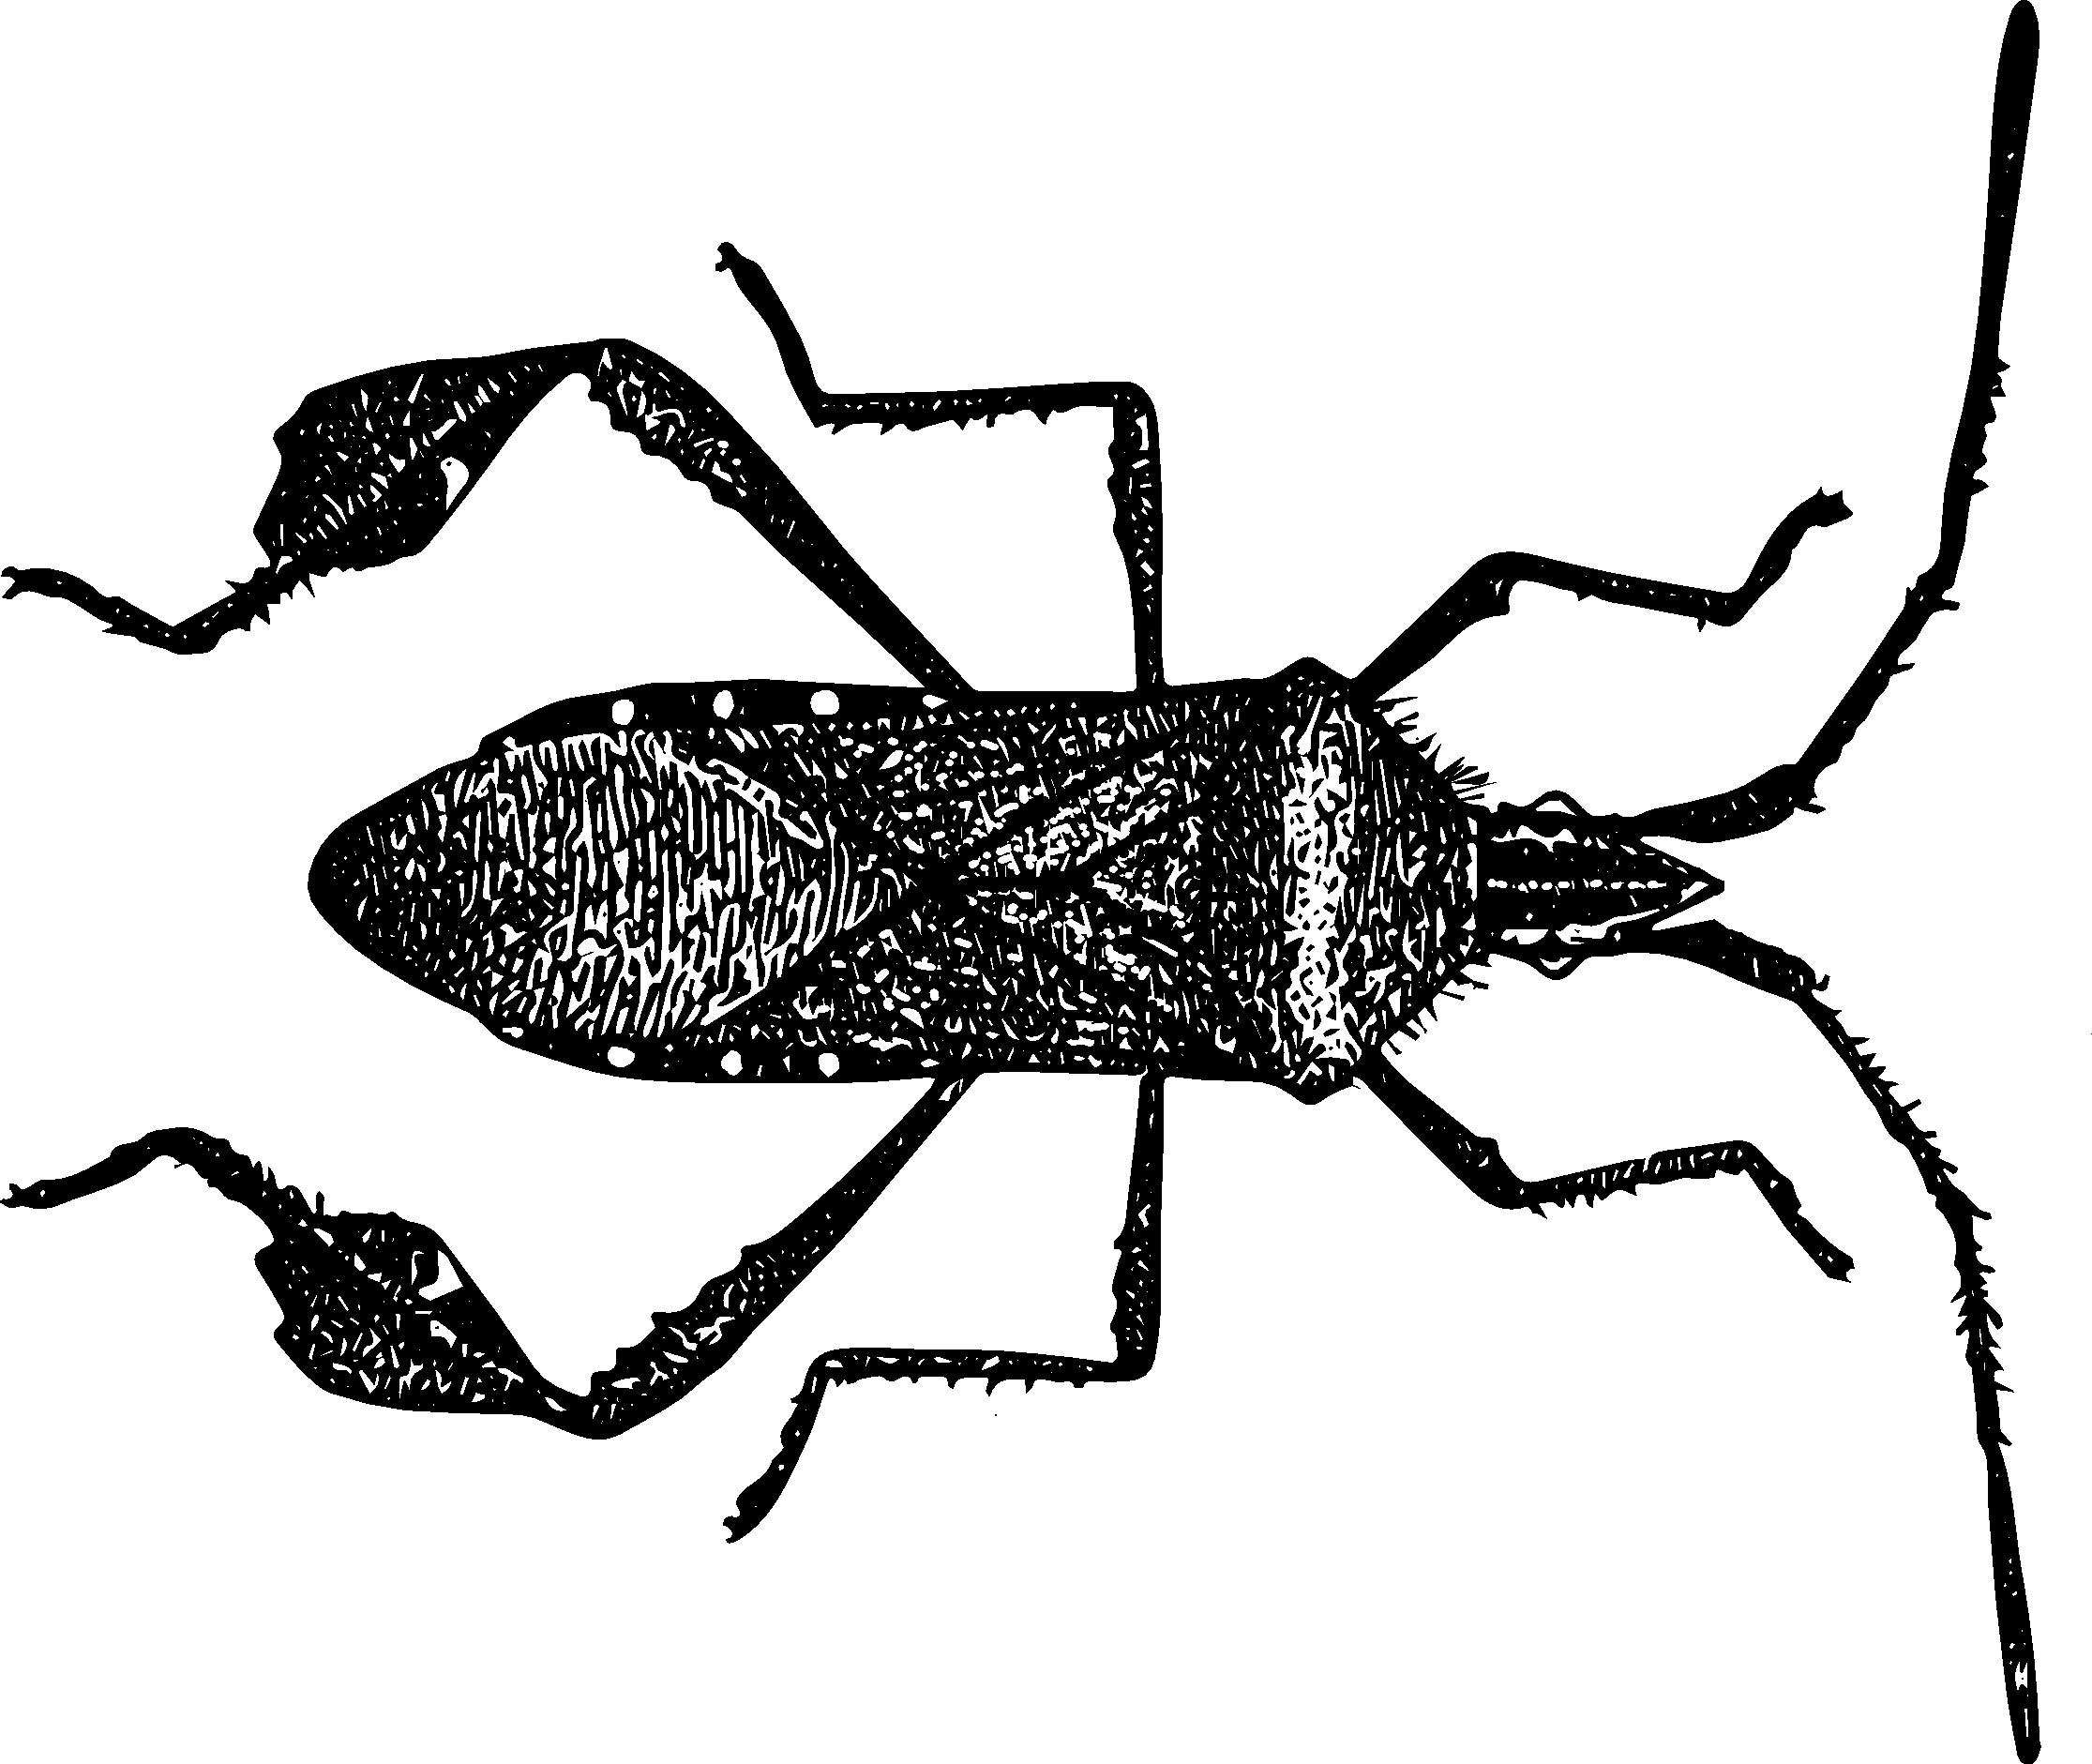
\includegraphics[width=\textwidth]{acercaria/coreidae}
  \caption{}
  \label{fig:coreid1}
 \end{subfigure}
 \caption{Coreidae. \textbf{(a)} Wing \citep[][Fig. 139-4]{bhlitem16791elementary}; \textbf{(b)} dorsal habitus \citep[][Fig. 9]{chittenden1899some}}\label{fig:coreids}
\end{figure}


\subsubsection{Aradidae (flat bugs)}\index{Aradidae}
\noindent{}\textit{Diagnostic characters:} Antenna with 4 antennomeres; number of labial sclerites: 4; ocelli absent; number of tarsomeres: 2; cuneus absent; fore leg not raptorial; wings short and wide, abdomen exposed distally and at most slightly exposed laterally; hind tibia usually widened, leaf-shaped; head narrower and shorter than pronotum.\vspace{3mm}

\noindent{}\textit{Natural history:} Almost 2,000 species have been described worldwide, and they are thought to be fungivores or saprophages. They have incredibly long stylets, which are coiled inside the body when not in use for feeding (figure \ref{fig:aradid2}).\vspace{3mm}

\begin{figure}[ht!]
 \centering
  \begin{subfigure}[ht!]{0.35\textwidth}
  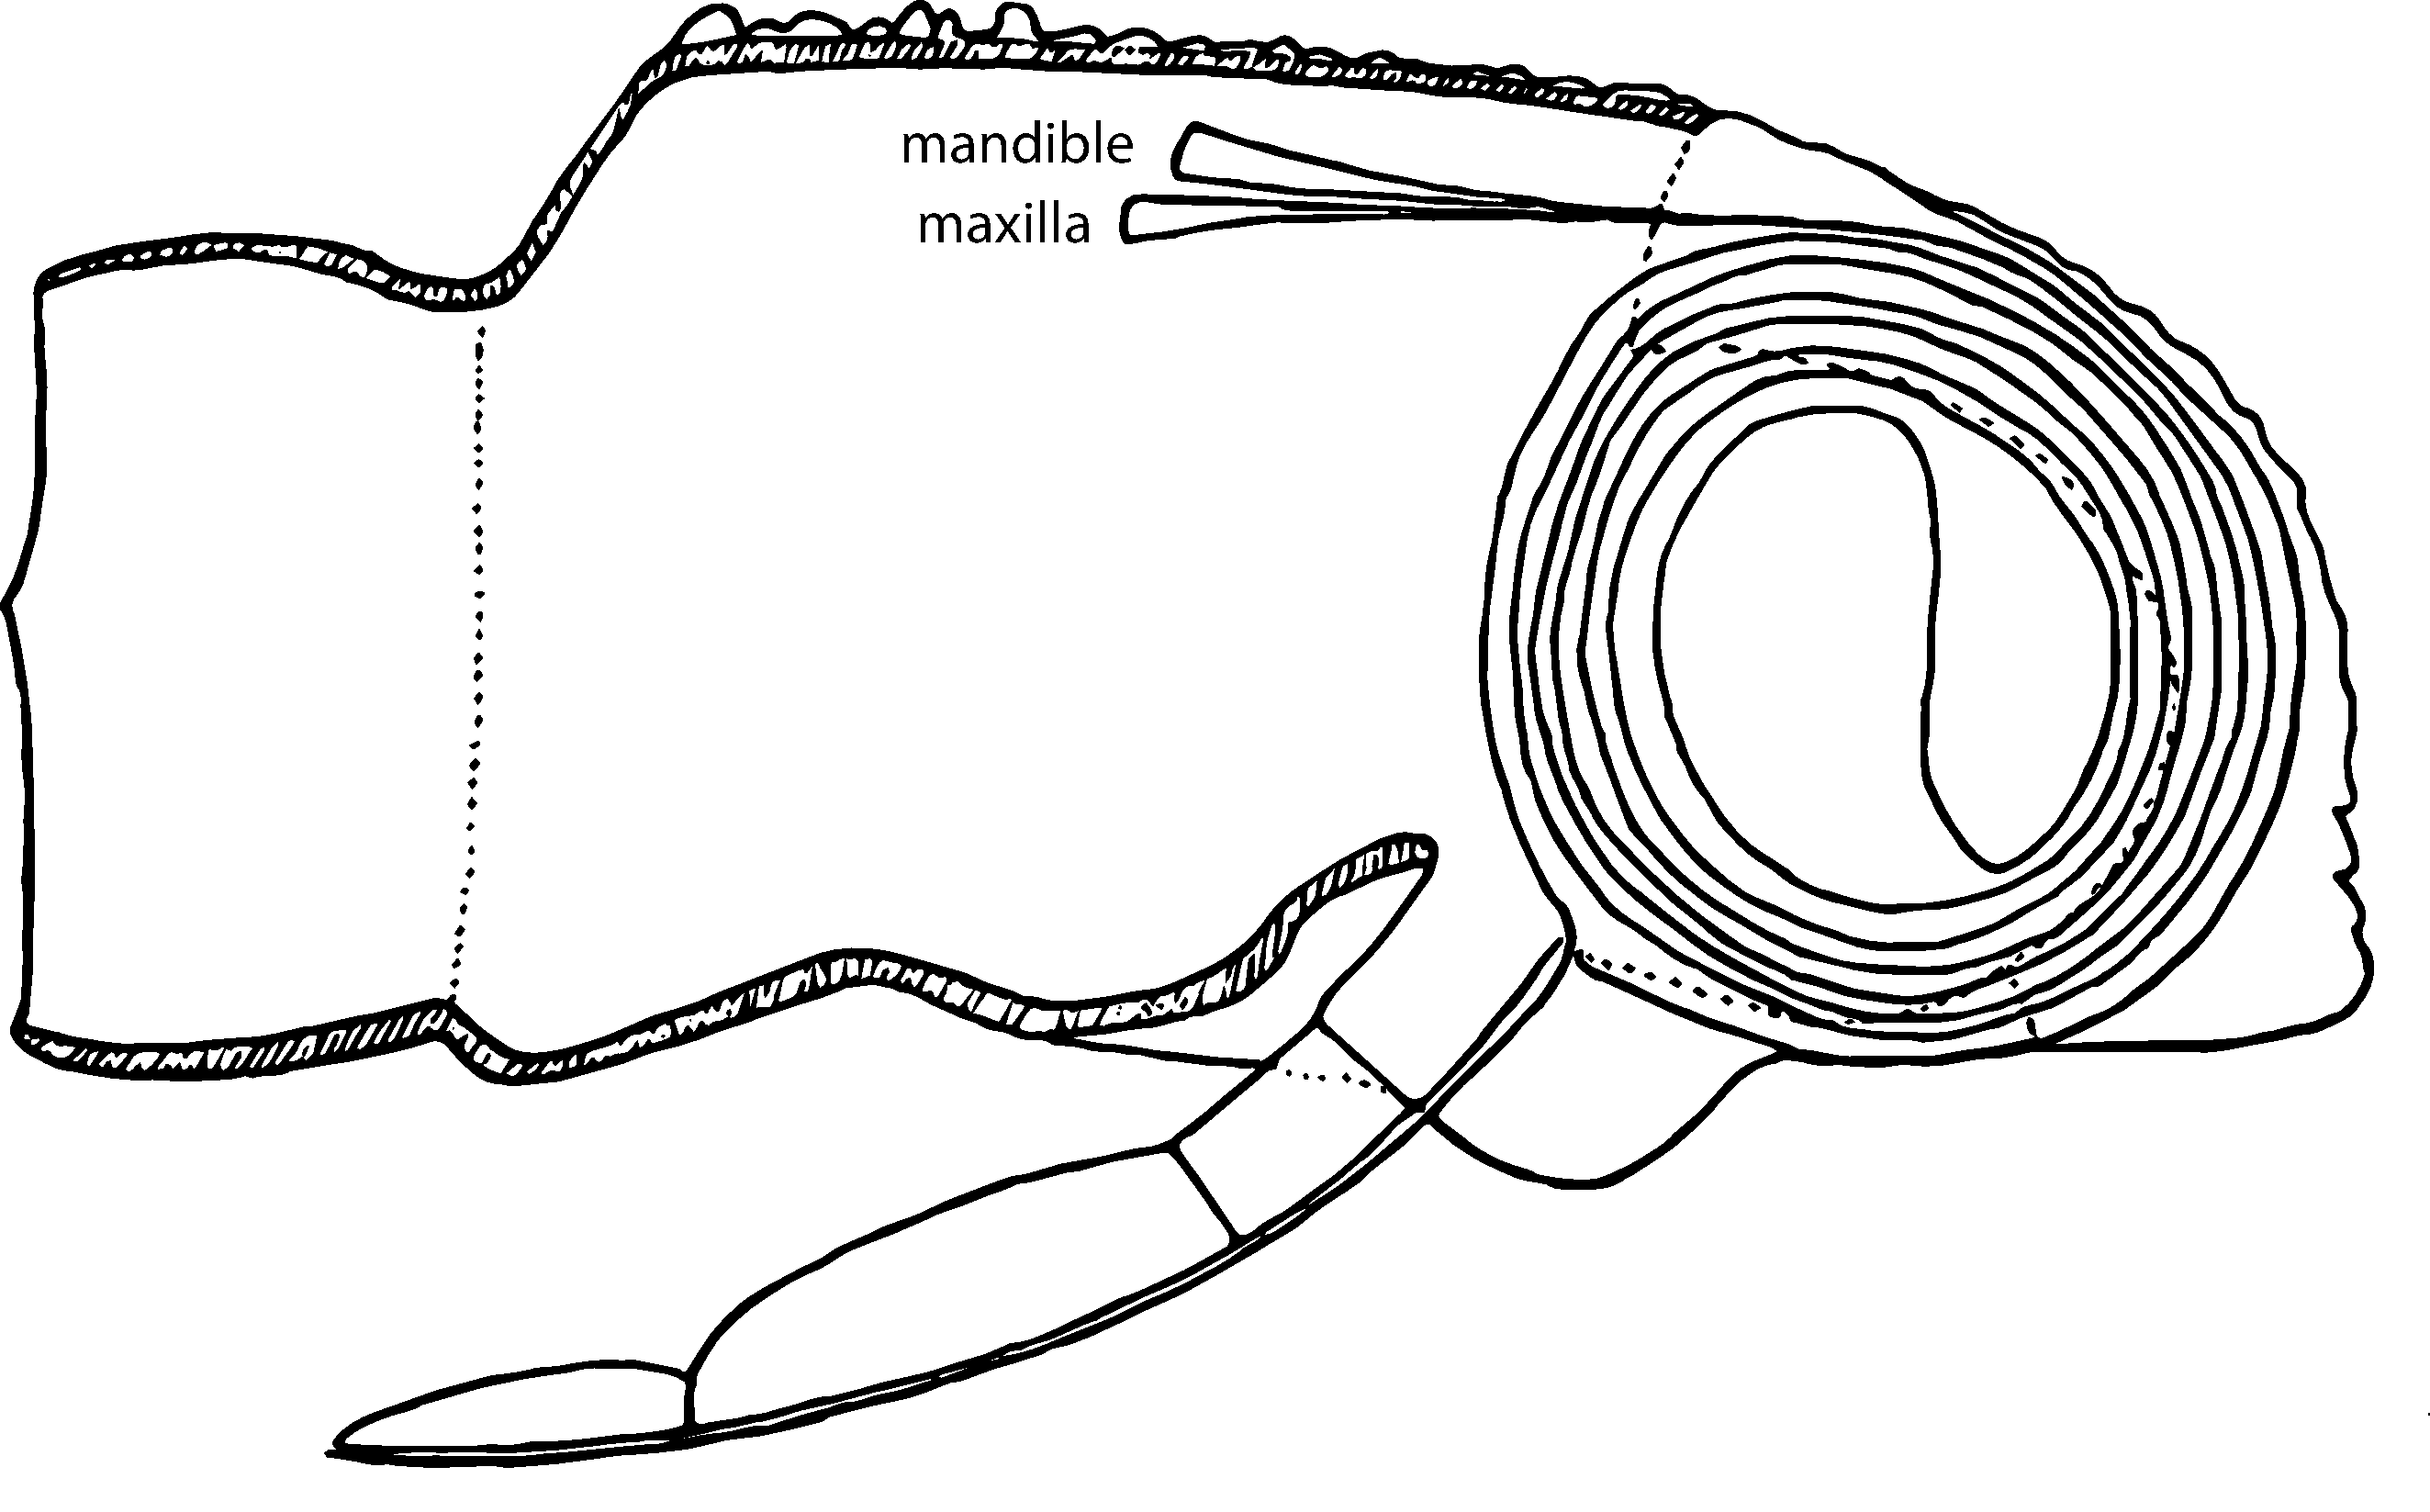
\includegraphics[width=\textwidth]{acercaria/aradidHead}
  \caption{}
  \label{fig:aradid2}
 \end{subfigure}
  \hfill
 \begin{subfigure}[ht!]{0.5\textwidth}
  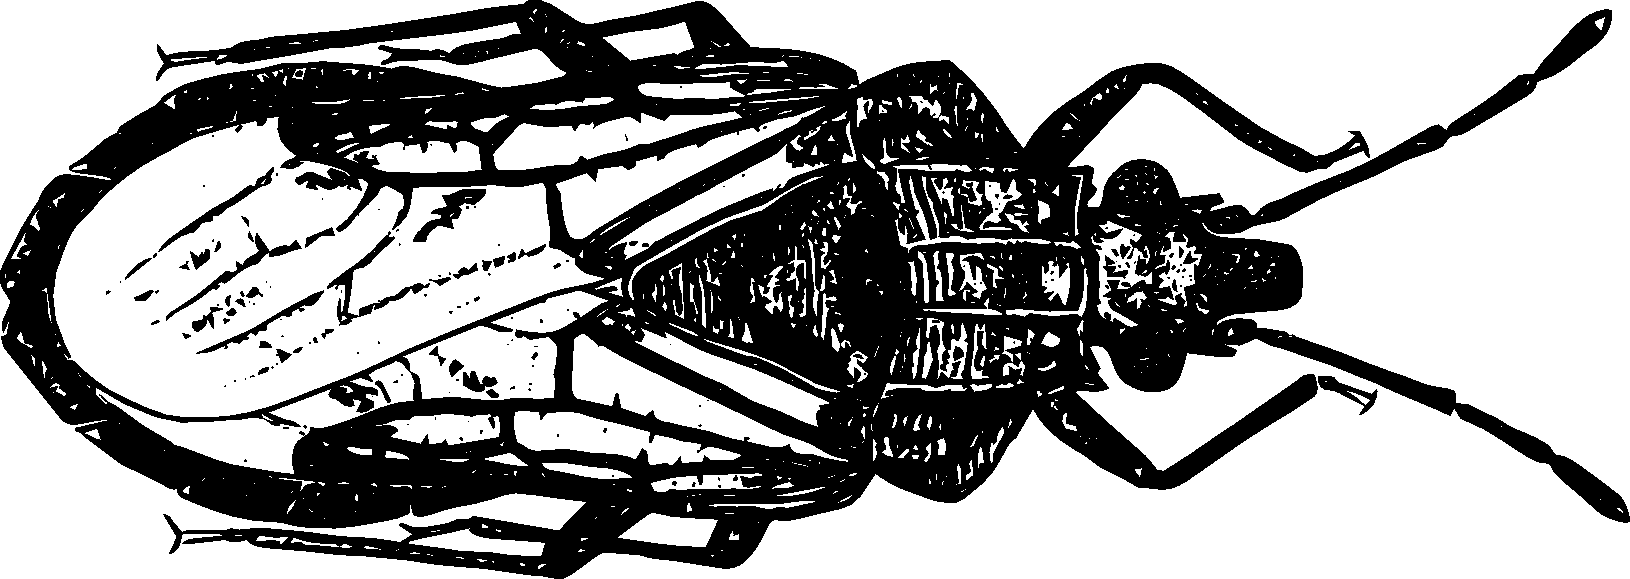
\includegraphics[width=\textwidth]{acercaria/aradid}
  \caption{}
  \label{fig:aradid1}
 \end{subfigure}
 \caption{Aradidae. \textbf{(a)} Inside of head, revealing coiled stylets \citep[redrawn from][Fig. 1]{Spooner121}; \textbf{(b)} habitus \citep[modified from][Fig. 1A]{deyrup2004natural}}\label{fig:aradids}
\end{figure}

\begin{theo}
{}Given their common name and their body shape, where do you think flat bugs live?
\end{theo}

\subsubsection{Scutelleridae (shield or shield-backed bugs)}\index{Scutelleridae}
\noindent{}\textit{Diagnostic characters:} Antenna with 5 antennomeres; labium with 4 sclerites; each leg with 3 tarsomeres; cuneus absent; mesoscutellum extends posteriorly, obscuring most of abdomen (figure \ref{fig:scutellerid1}); wings wide, abdomen at most slightly exposed laterally.\vspace{3mm}

\noindent{}\textit{Natural history:} About 450 species of shield bugs have been described worldwide. All species are phytophagous, and some exhibit traumatic insemination.\vspace{3mm}

\begin{figure}[ht!]
 \centering
\begin{subfigure}[ht!]{0.32\textwidth}
 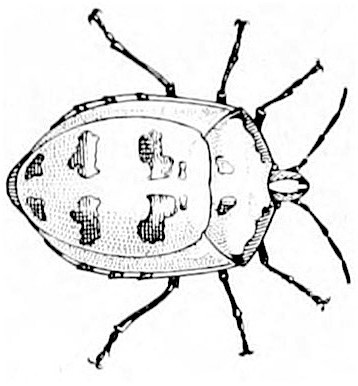
\includegraphics[width=\textwidth]{acercaria/ScutelleridHabitus}
 \caption{Scutelleridae}
 \label{fig:scutellerid1}
\end{subfigure}
 \hfill 
\begin{subfigure}[ht!]{0.48\textwidth}
 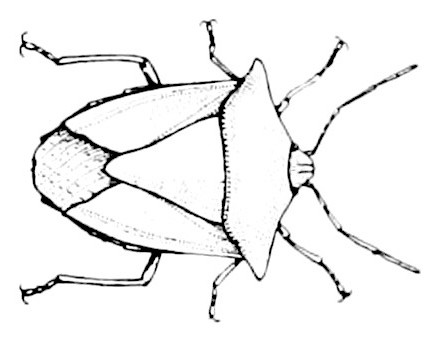
\includegraphics[width=\textwidth]{acercaria/PentatomidHabitus}
 \caption{Pentatomidae}
 \label{fig:pentatomid1}
\end{subfigure}
 \caption{\textbf{(a)} Scutelleridae habitus \citep[redrawn from][Plate XXXI, Fig. 11]{bhlitem82061AustrInsect}; \textbf{(b)} Pentatomidae habitus \citep[][Fig. 44]{bhlitem105840ross}}\label{fig:pentscut}
\end{figure}

\subsubsection{Pentatomidae (stink bugs)}\index{Pentatomidae}
\noindent{}\textit{Diagnostic characters:} antenna with 5 antennomeres (figure \ref{fig:pentatomid1}); labium with 4 sclerites; each leg with 3 tarsomeres; cuneus absent; mesoscutellum extends posteriorly but does not obscure most of abdomen; fore leg not raptorial; wings wide, abdomen at most slightly exposed laterally.\vspace{3mm}

\noindent{}\textit{Natural history:} About 5,000 species have been described worldwide. Most species are herbivores but many predate on other insects and can be effective biocontrol agents.\vspace{3mm}

\section{Psocodea (lice)}\index{Psocodea}
This lineage is comprised of three infraorders. Older classifications---Phthiraptera for parasitic lice and Psocoptera for bark lice, for example---resulted in at least one polyphyletic taxon. Synapomorphies of Psocodea include: Specialized water vapor uptake system (sitophore); autotomic antennae (look for a line of weakness proximally); molecular data.\vspace{3mm}

\subsection{Psocomorpha (bark lice)}\index{Psocomorpha}
\noindent{}\textit{Diagnostic characters:} Head usually with rounded vertex; antenna with 13 antennomeres; flagellomeres never annulated; labial palpus not subdivided; fore wing with nodus and thickened pterostigma (figure \ref{fig:psocids}); CuP ending together with A1 at wing margin; tarsus subdivided into 2--3 tarsomeres.\vspace{3mm}

\noindent{}There are 24 families classified in Psocomorpha).

\begin{figure}[ht!]
 \centering
\begin{subfigure}[ht!]{0.45\textwidth}
 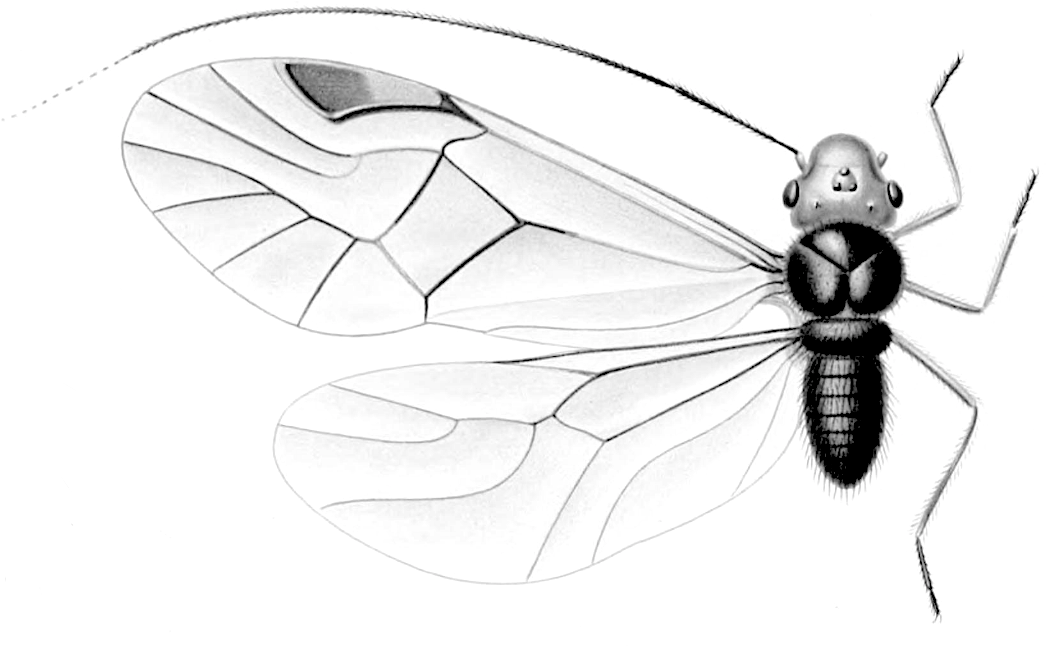
\includegraphics[width=\textwidth]{acercaria/psocomorphan}
 \caption{}
 \label{fig:psocids}
\end{subfigure}
 \hfill 
\begin{subfigure}[ht!]{0.5\textwidth}
 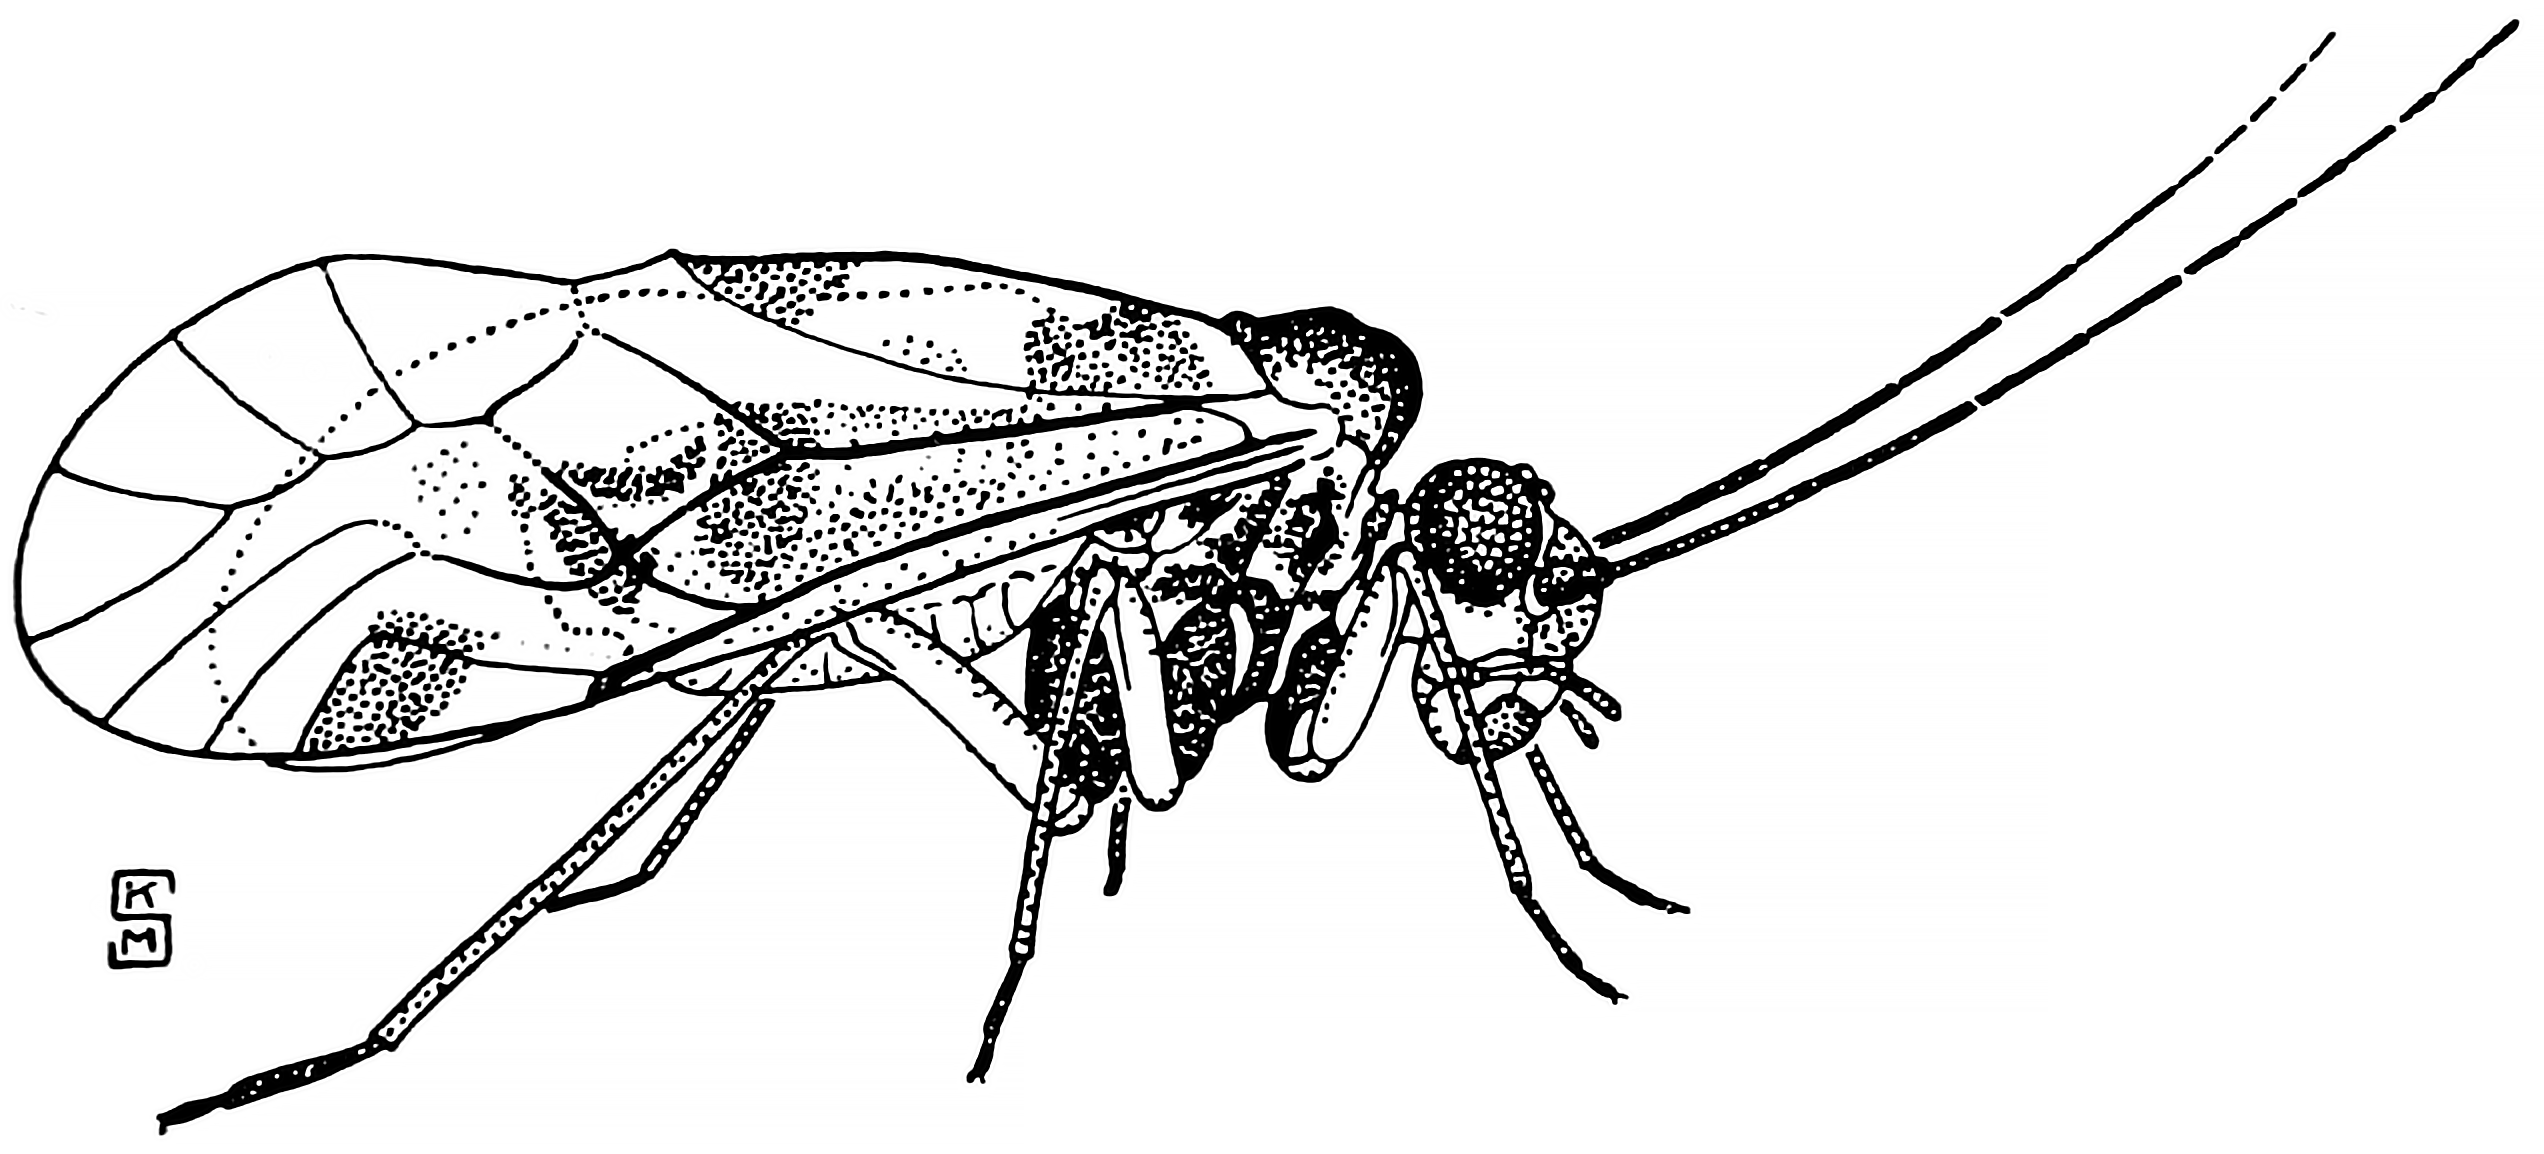
\includegraphics[width=\textwidth]{acercaria/Psocomorpha}
 \caption{}
 \label{fig:psocids1}
\end{subfigure}
 \caption{Psocomorpha. \textbf{(a)} dorsal habitus \citep[][Fig. 19]{bhlitem37577}; \textbf{(b)} lateral habitus \citep[][Fig. 40]{bhlitem105840ross}}\label{fig:psocids2}
\end{figure}


\subsection{Troctomorpha (book and parasitic lice)}\index{Troctomorpha}
\noindent{}\textit{Diagnostic characters:} Head usually with relatively flat vertex; antenna with 15--17 antennomeres; tarsus subdivided into 2 tarsomeres.\vspace{3mm}

\noindent{}There are 9 families classified in Troctomorpha. In lab we will look at four (see below), all of which are wingless and three of which are parasitic.

\subsubsection{Liposcelididae (common book lice)}\index{Liposcelididae}
\noindent{}\textit{Diagnostic characters:} Body usually yellow-brown in color; head prognathous; antenna relatively long, with 9--15 flagellomeres (figure \ref{fig:liposcelidid}); tarsus subdivided into 3 tarsomeres; hind femora relatively large; wings absent in most species.\vspace{3mm}

\noindent{}\textit{Natural history:} These insects can frequently be found on books, in leaf litter, or as pests of stored products (grains, flour). Approximately 200 species are known worldwide, and several are closely associated with birds and mammals.\vspace{3mm}

\begin{figure}[ht!]
 \centering
 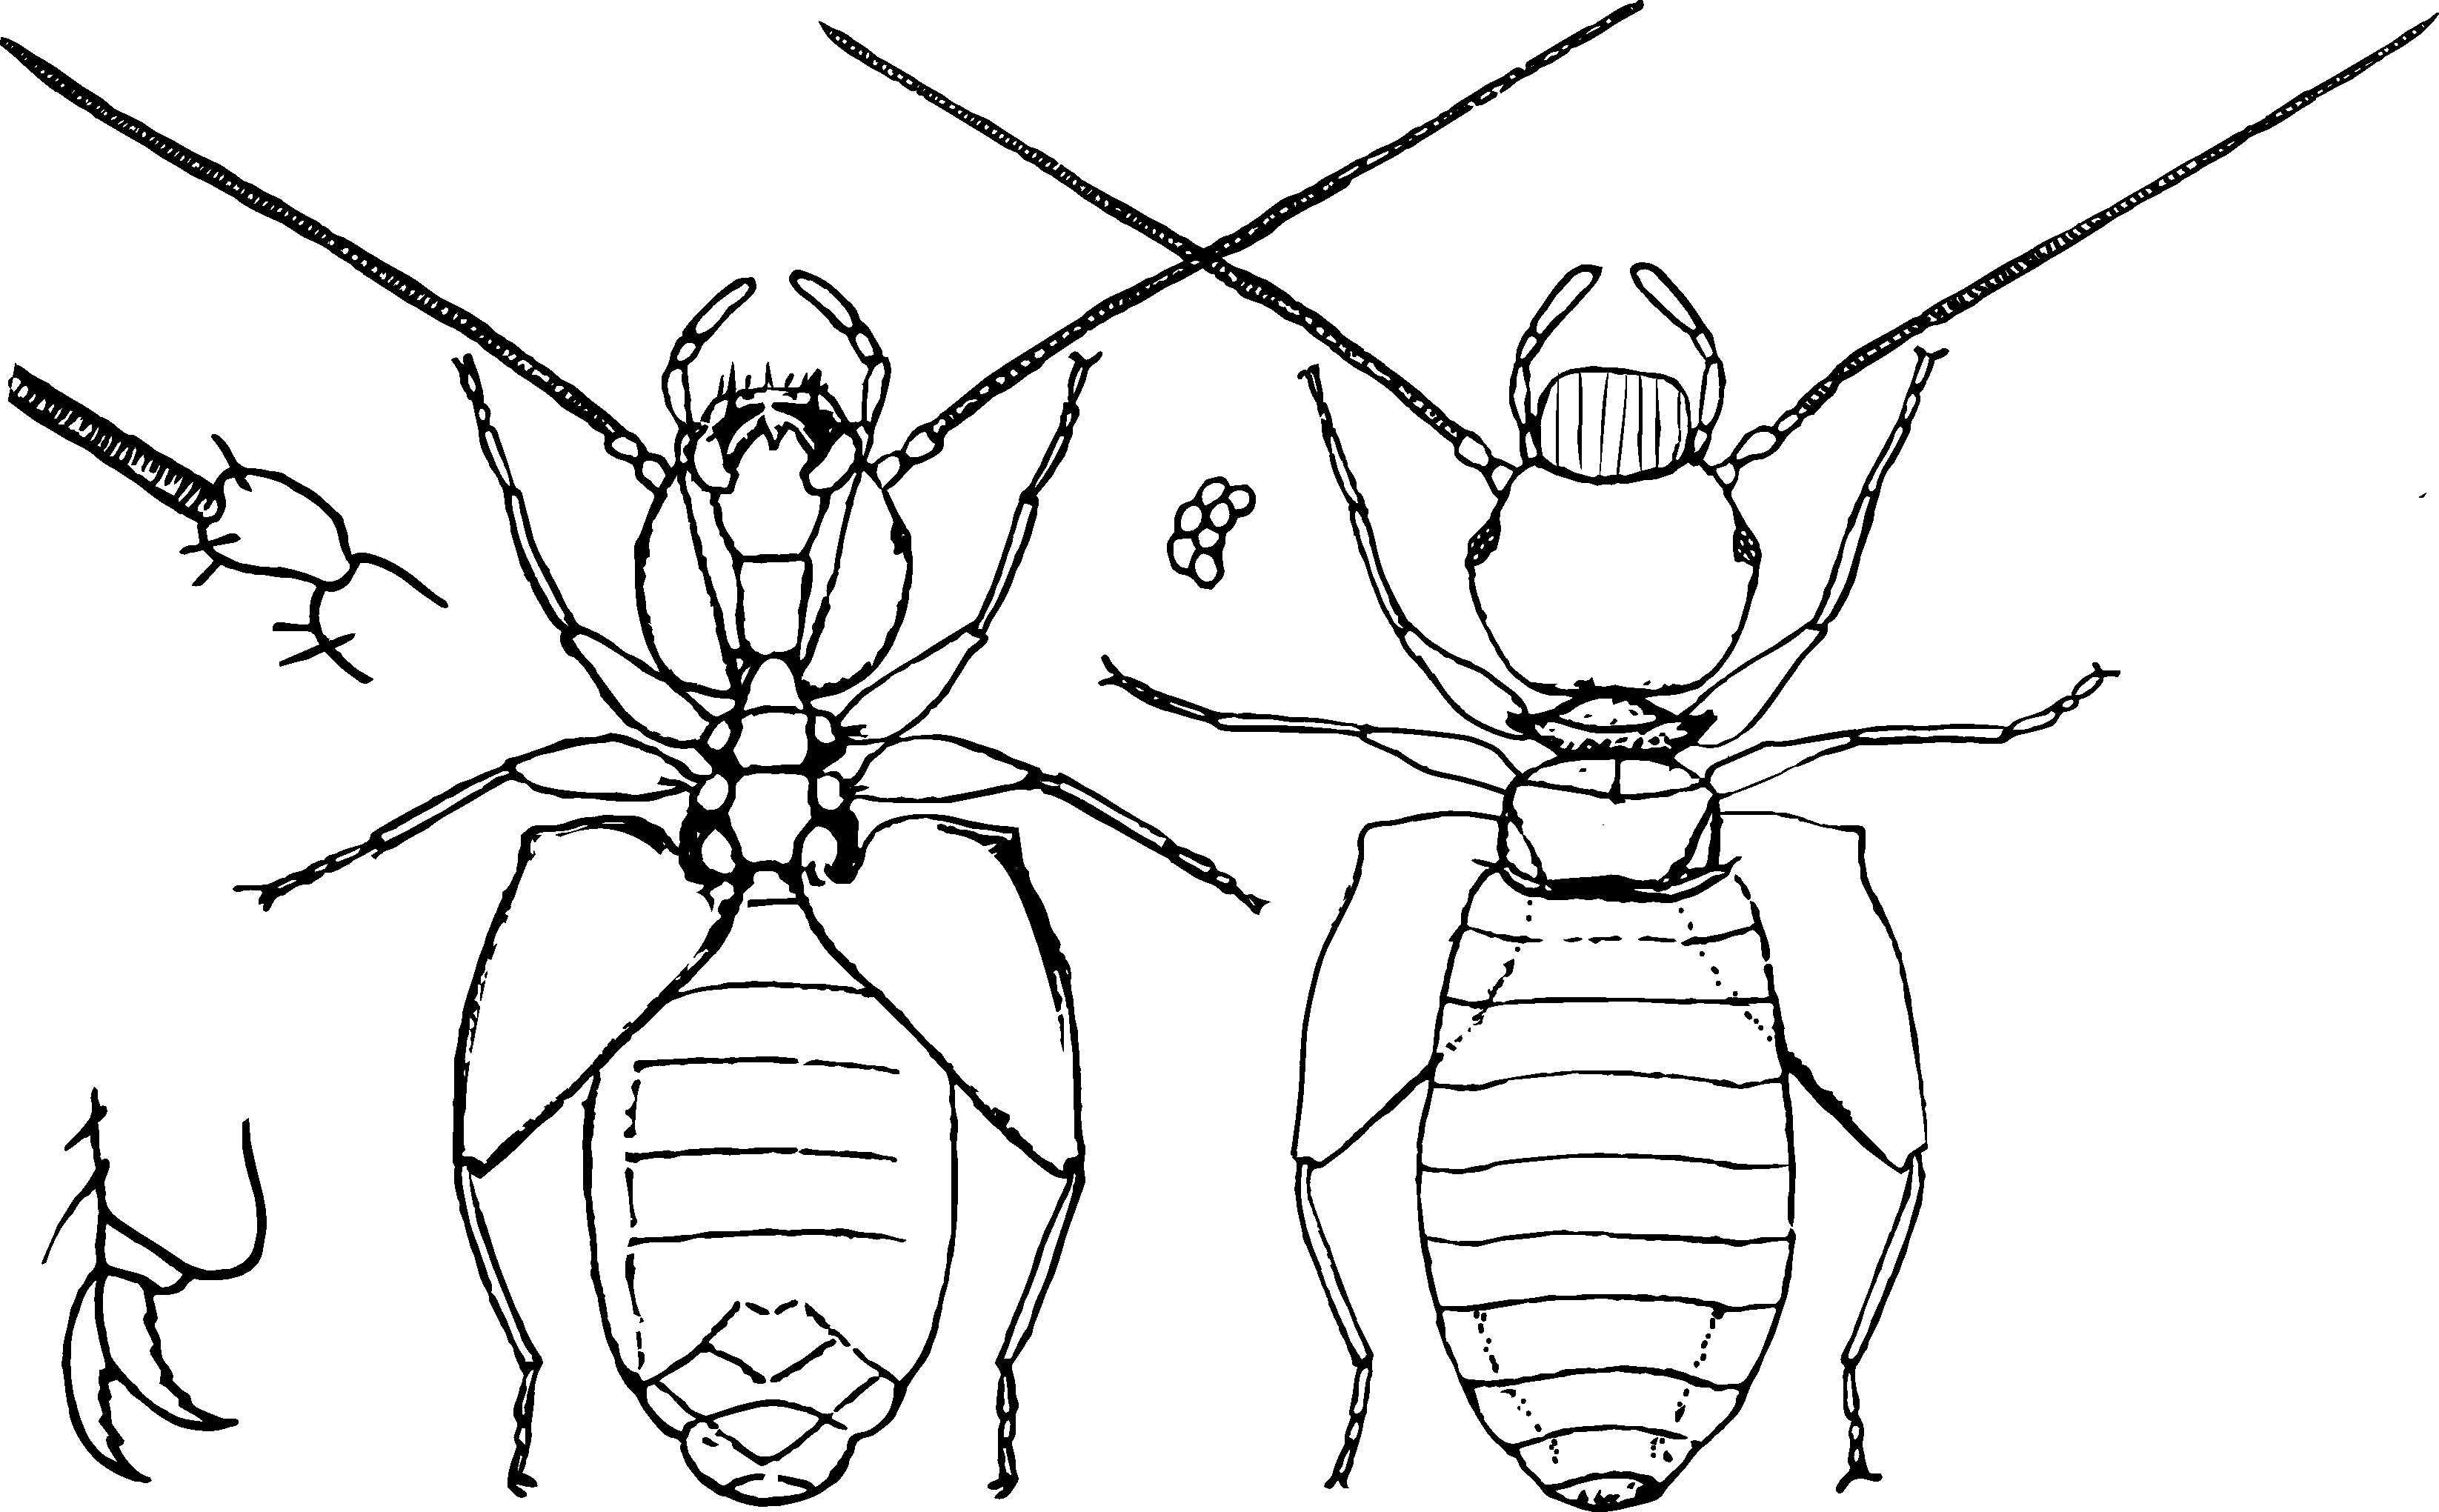
\includegraphics[width=0.58\textwidth]{acercaria/liposcelidid}
 \caption{Liposcelididae \citep[redrawn from][Fig. 34]{Howard029686434}}
 \label{fig:liposcelidid}
\end{figure}

\subsubsection{Pediculidae (human head and body lice)}\index{Pediculidae}
\noindent{}\textit{Diagnostic characters:} Head usually narrower than prothorax (figure \ref{fig:pediculid}); fore, mid, and hind legs roughly equal in size; tibial-tarsal complex adapted for grabbing; abdomen longer than width at base.\vspace{3mm}

\noindent{}\textit{Natural history:} These lice feed via piercing-sucking mouthparts and are classified in Anoplura (sucking lice). There are six described species worldwide, and all are parasites of Primates. This family include the human body and head lice species.\vspace{3mm}

\begin{figure}[ht!]
 \centering
 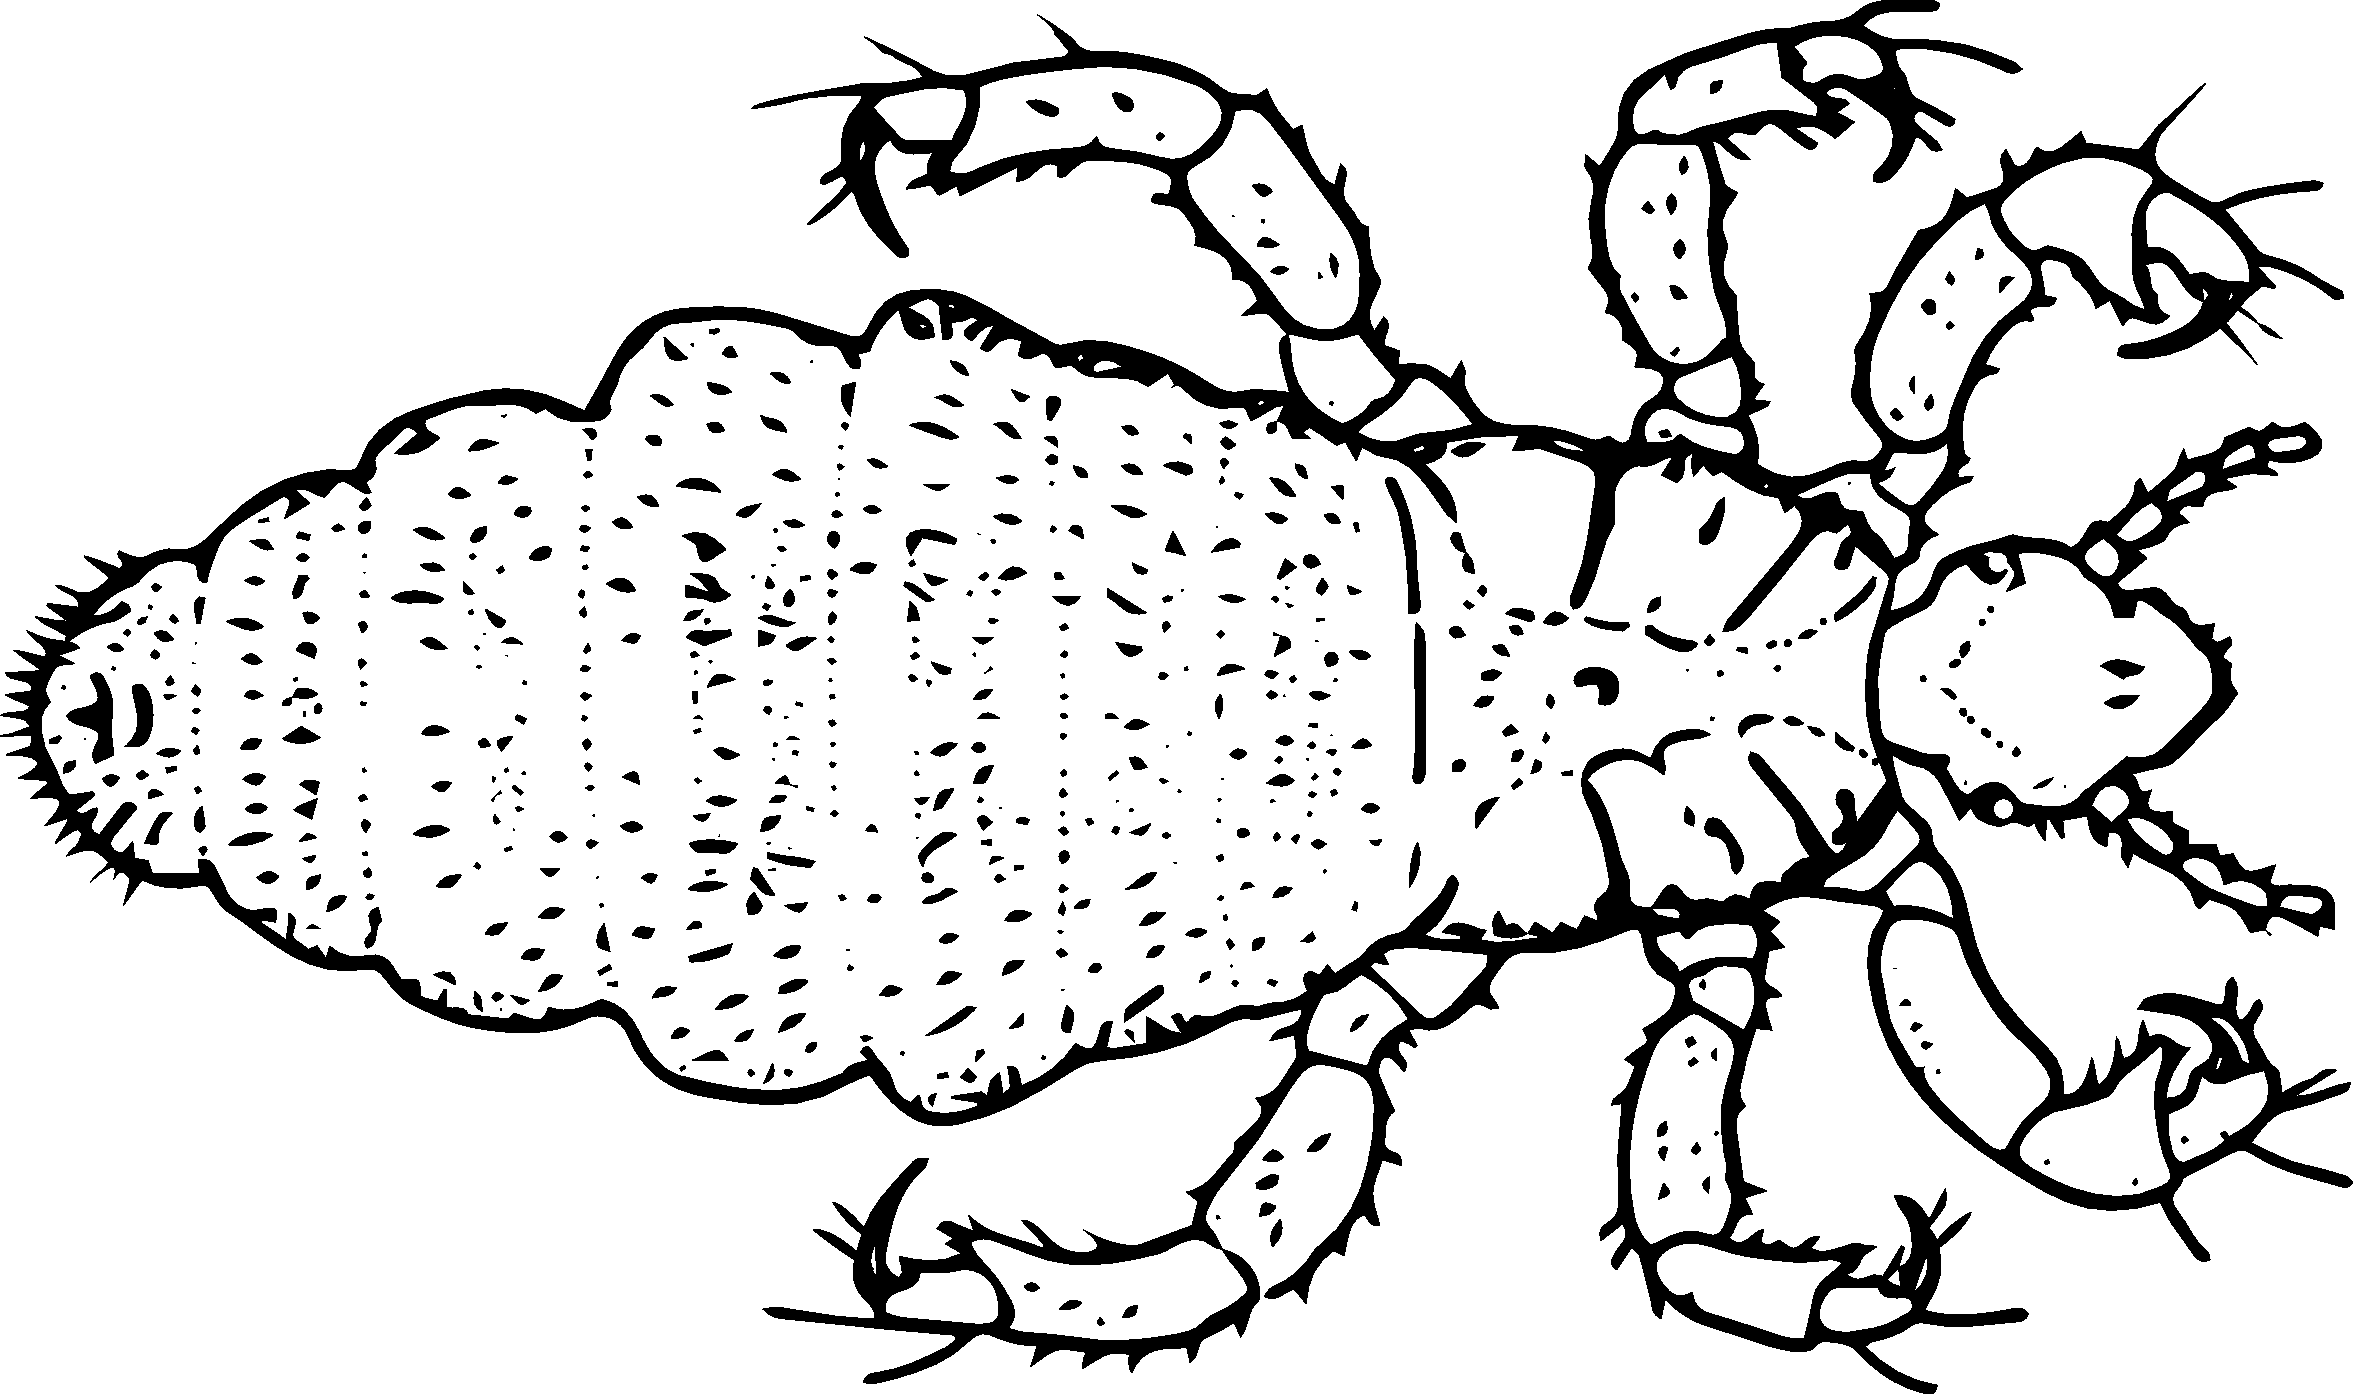
\includegraphics[width=0.38\textwidth]{acercaria/Pediculidae}
 \caption{Pediculidae \citep[redrawn from][Fig. 13A]{snodgrass1944feeding}}
 \label{fig:pediculid}
\end{figure}

\subsubsection{Phthiridae (human pubic louse, gorilla louse)}\index{Phthiridae}
\noindent{}\textit{Diagnostic characters:} Head narrower than prothorax; mid and hind legs thicker than fore legs; abdomen about as long as its width at base, with prominent lobe-like structures (paratergites) laterally (figure \ref{fig:phthirid}).\vspace{3mm}

\noindent{}\textit{Natural history:} There are only two described species in this family, which is also classified in Anoplura. One is \textit{Phthirus pubis} (Linnaeus, 1758), the human pubic louse. The other species is a parasite of gorillas (\textit{Gorilla gorilla} (Savage, 1847)).\vspace{3mm}

\begin{figure}[ht!]
 \centering
 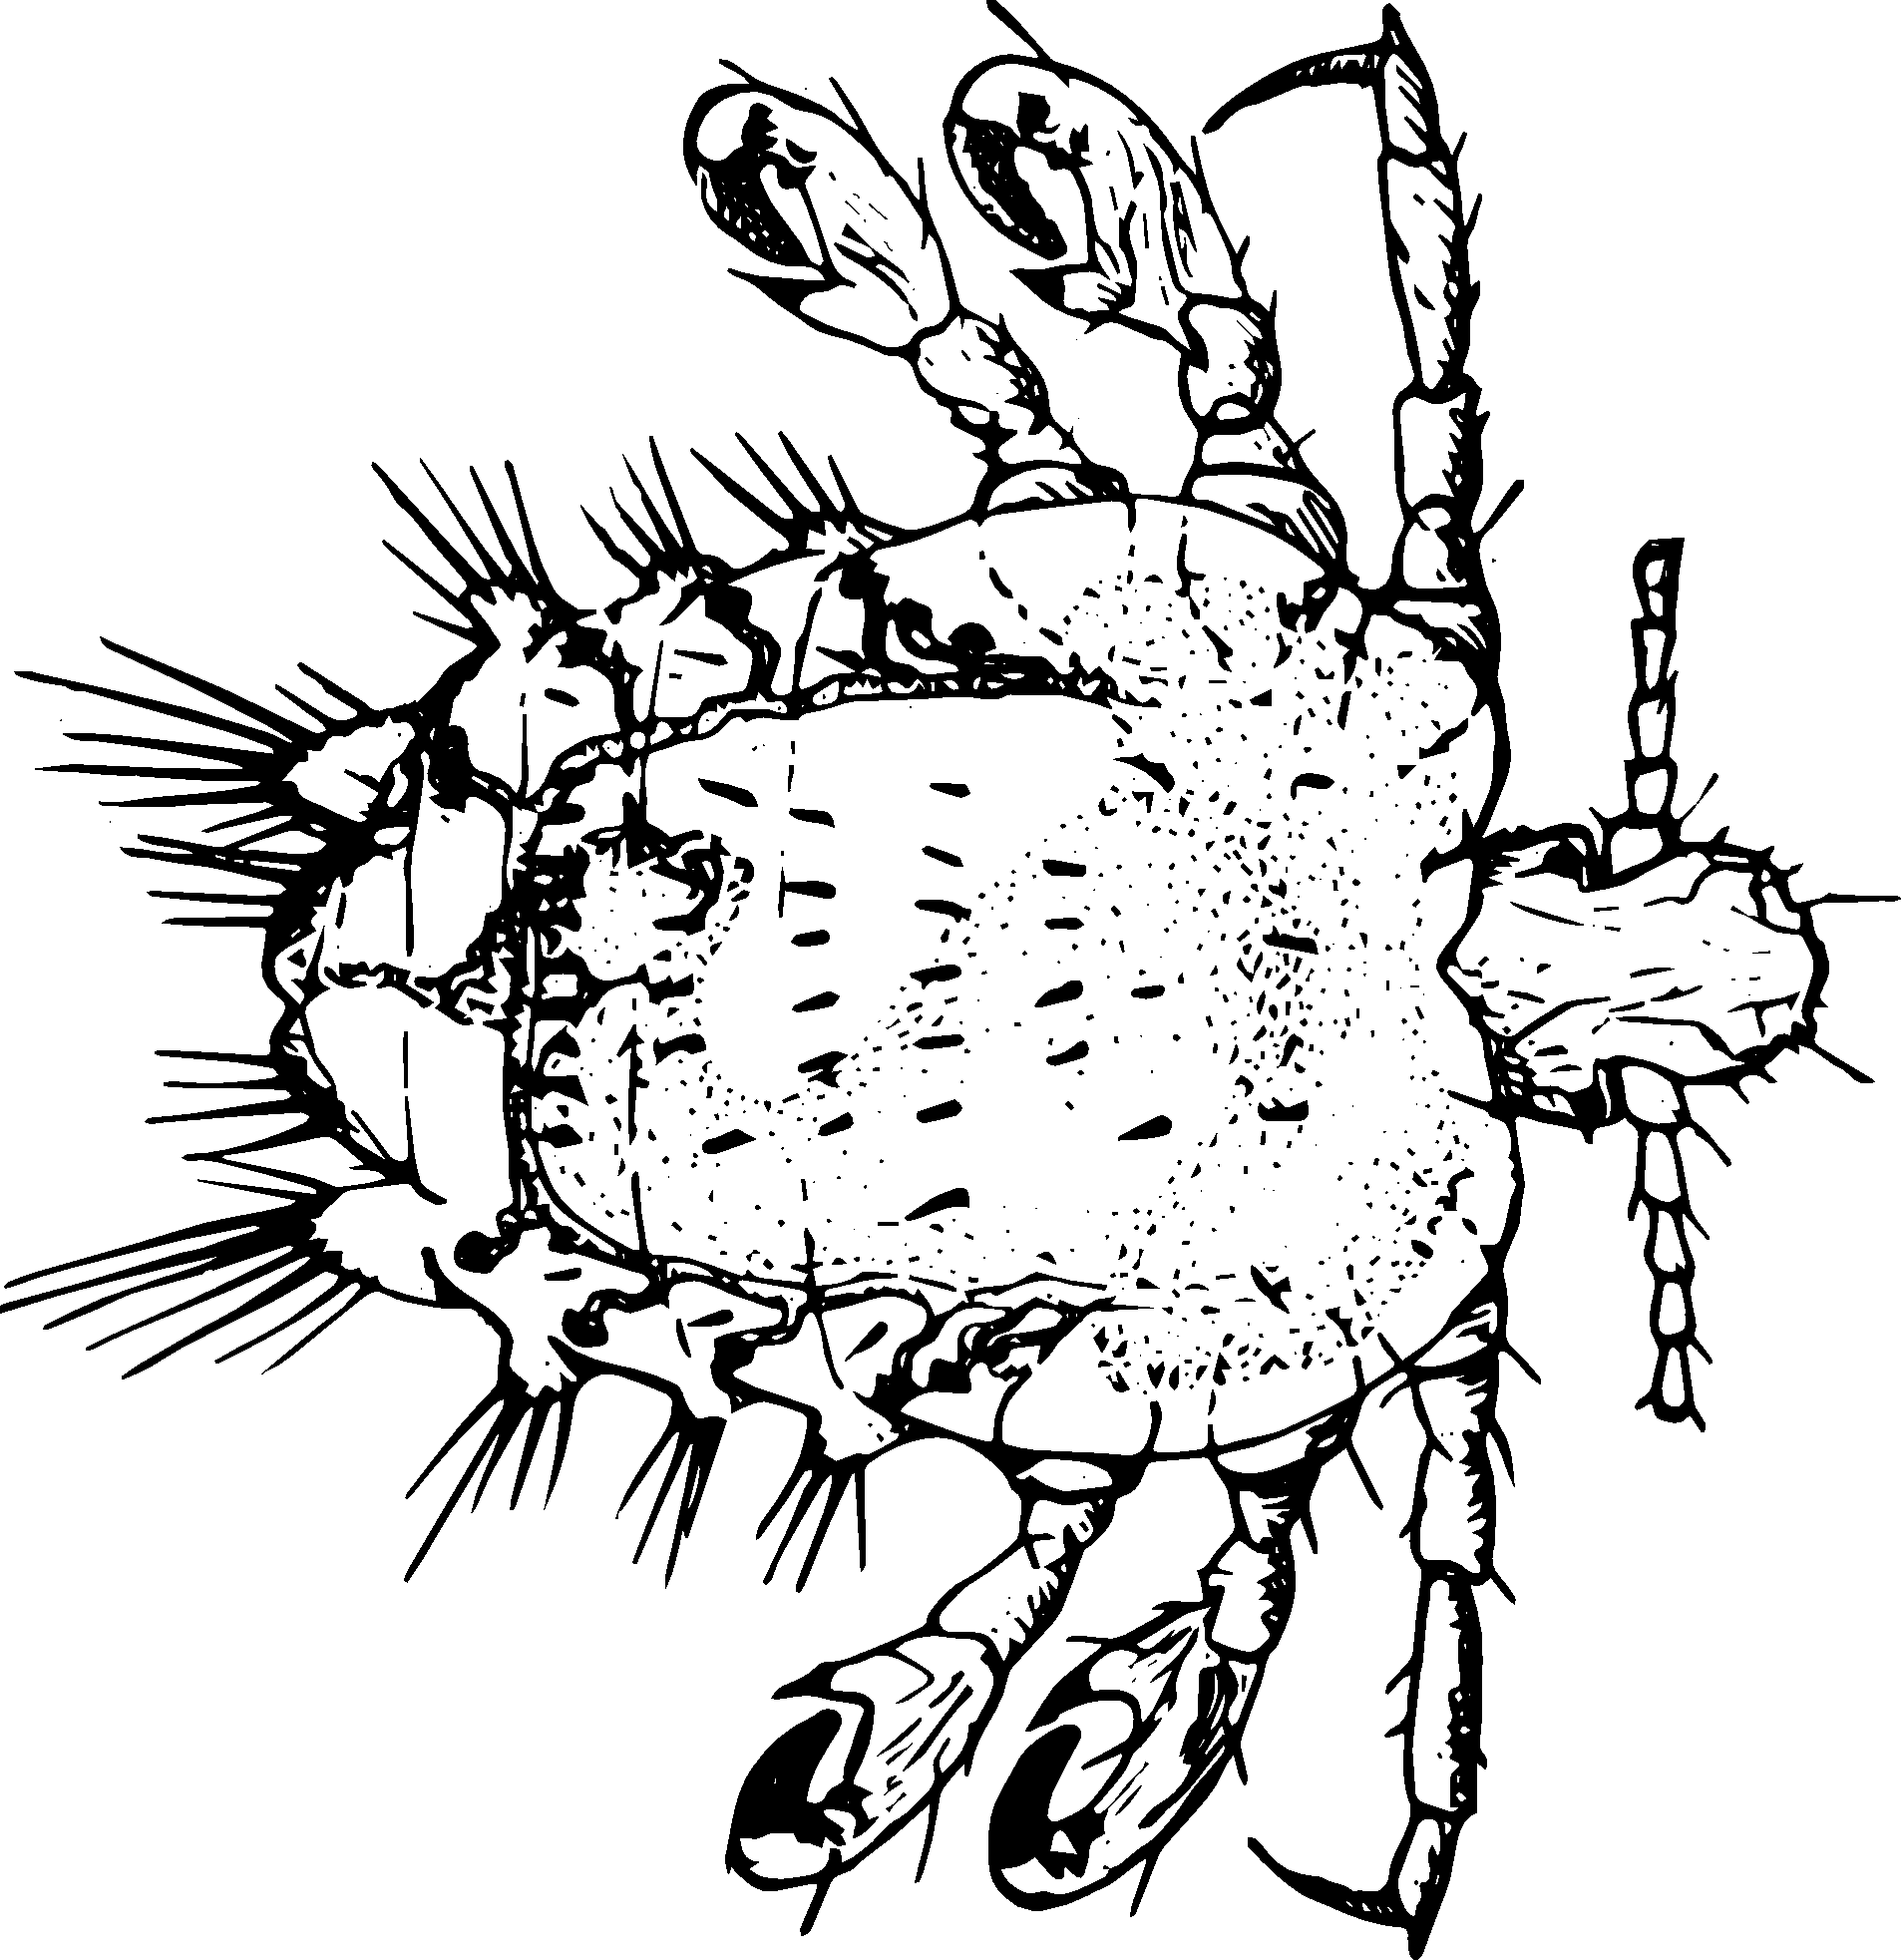
\includegraphics[width=0.33\textwidth]{acercaria/phthirid1}
 \caption{Phthiridae \citep[redrawn from][Fig. 176]{chandler1922animal}}
 \label{fig:phthirid}
\end{figure}

\subsubsection{Trichodectidae (mammal chewing lice)}\index{Trichodectidae}
\noindent{}\textit{Diagnostic characters:} Head as wide as or wider than thorax; mouthparts chewing (mandibulate) (figure \ref{fig:trichodectid}); antennae filiform, exposed, with 3 antennomeres; maxillary palpi absent.\vspace{3mm}

\noindent{}\textit{Natural history:} More than 400 trichodectid species have been described worldwide, all of which are parasites of mammals. They feed via chewing mouthparts and historically have been classified in a polyphyletic higher-level taxon ``Mallophaga''.\vspace{3mm}

\begin{figure}[ht!]
 \centering
 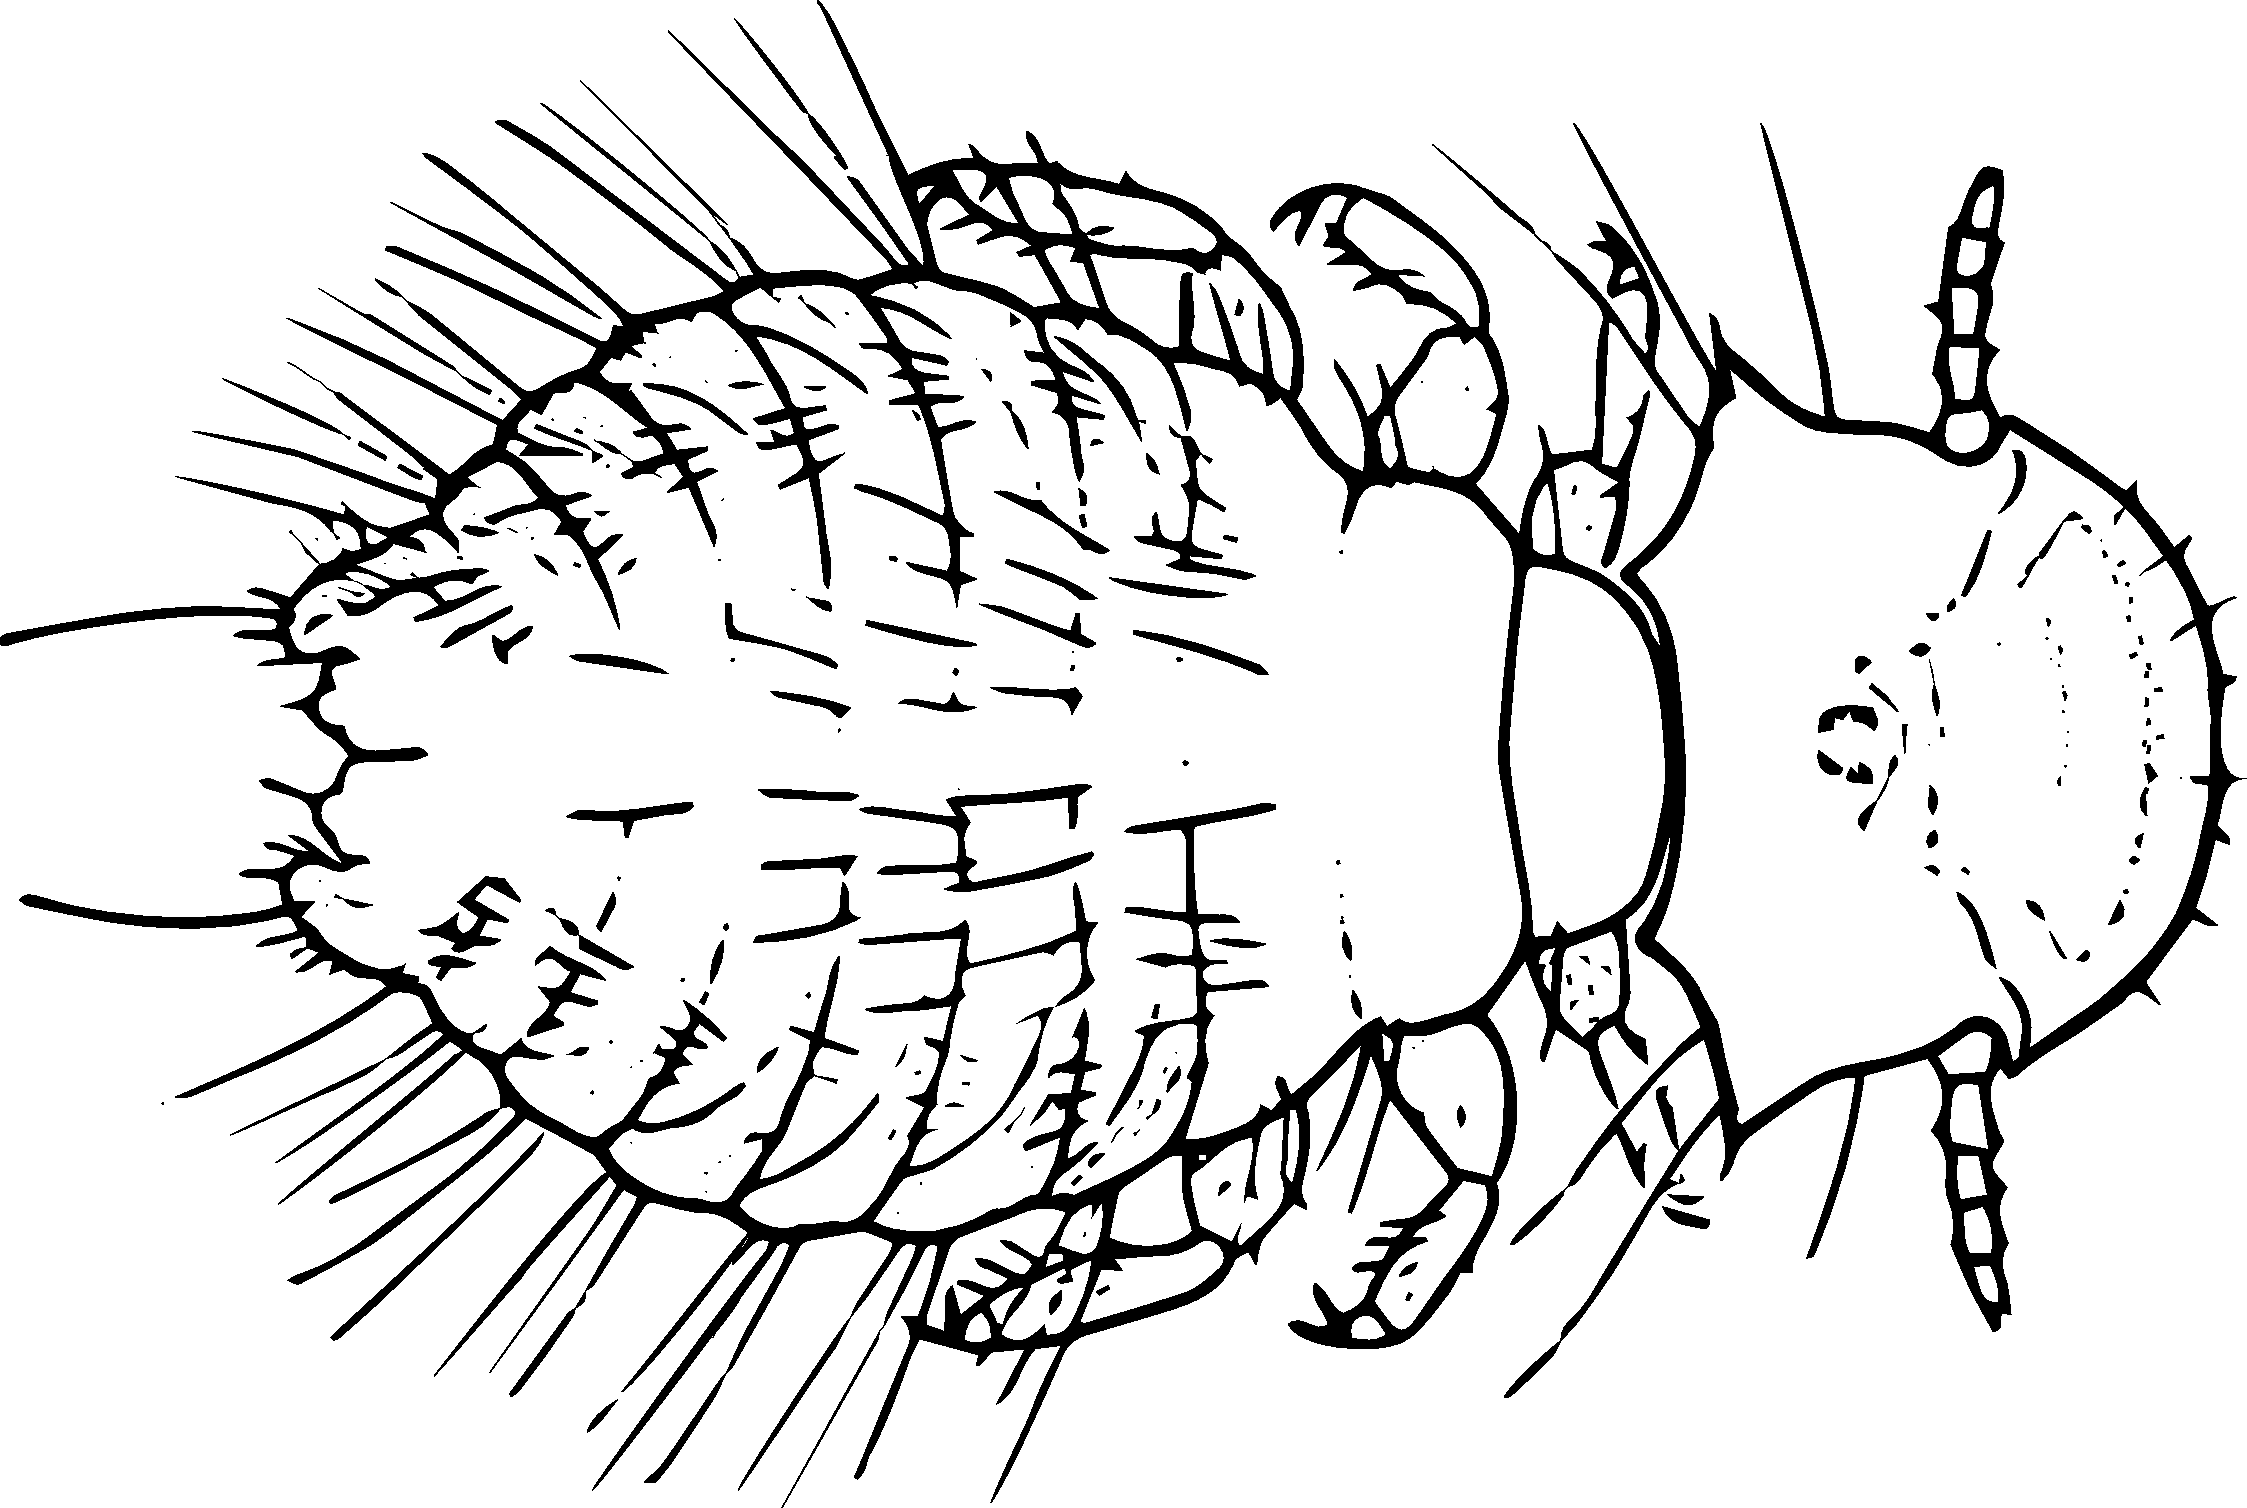
\includegraphics[width=0.38\textwidth]{acercaria/trichodectidae}
 \caption{Trichodectidae, ventral habitus \citep[redrawn from][Fig. 9B]{snodgrass1944feeding}}
 \label{fig:trichodectid}
\end{figure}

\subsection{Trogiomorpha}\index{Trogiomorpha}
\noindent{}\textit{Diagnostic characters:} Antenna with 22--50 antennomeres; forewing pterostigma is not thickened but rather is transparent to slightly opaque.\vspace{3mm}

\noindent{}There are 7 families classified in Trogiomorpha, which covers at least 300 species worldwide. We have no specimens in our teaching collection, but the lineage is included here because several species are pests of stored products.\vspace{3mm}

\begin{theo}
{}Compare the parasitic psocodeans to those that live on bark or in leaf litter. What adaptations can you observe that you hypothesize are for parasitization? Compare head shape and size, between Trichodectidae and Anoplura. Why are they different?
\end{theo}

\section{Thysanoptera (thrips)}\index{Thysanoptera}
\noindent{}\textit{Diagnostic characters:} Body very small (usually $\sim$2 mm), with opisthognathous head; antenna with 7--9 antennomeres; piercing/sucking, asymmetrical (one mandible present) mouthparts; wings usually narrow with fringe composed of long setae; fore wing similar in size/shape to hind wing; tarsus with 1 or 2 tarsomeres; arolium (apicomedial membraneous area of pretarsus) balloon-shaped, eversible, exceeds tarsal claw apically.\vspace{3mm}

\noindent{}Thysanoptera is subdivided into two suborders---Terebrantia (8 families, including Thripidae) and Tubulifera (1 family; Phlaeothripidae). Keep in mind that ``thrips'' is both singular and plural!

\subsection{Terebrantia}\index{Terebrantia}%learn as suborder instead of family?
\subsubsection{Thripidae (common thrips)}\index{Thripidae}
\noindent{}\textit{Diagnostic characters:} terminal abdominal segment divided ventrally, cone shaped, with strongly converging lateral margins; ovipositor present (figure \ref{fig:thripid2}), saw-like and curving ventrally; wing surface with acanthae (microtrichiae, or cuticular protuberances in the wing) and 2 rows of setae.\vspace{3mm}

\noindent{}\textit{Natural history:} More than 2,000 species have been described worldwide, including many pestiferous species. Most species survive as cryptophilous herbivores. As with many other kinds of thrips, some species are facultative parasites.\vspace{3mm}

\begin{figure}[ht!]
 \centering
 \begin{subfigure}[ht!]{0.48\textwidth}
  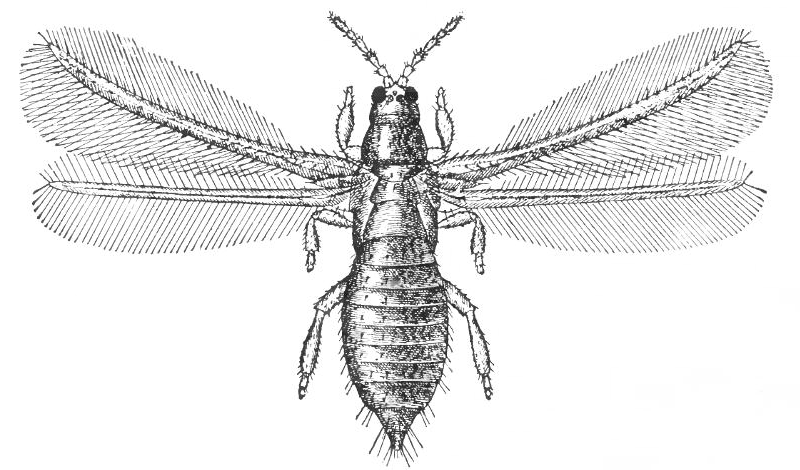
\includegraphics[width=\textwidth]{acercaria/ThripidHabitus}
  \caption{}
  \label{fig:thripid1}
 \end{subfigure}
 \qquad
 \begin{subfigure}[ht!]{0.32\textwidth}
      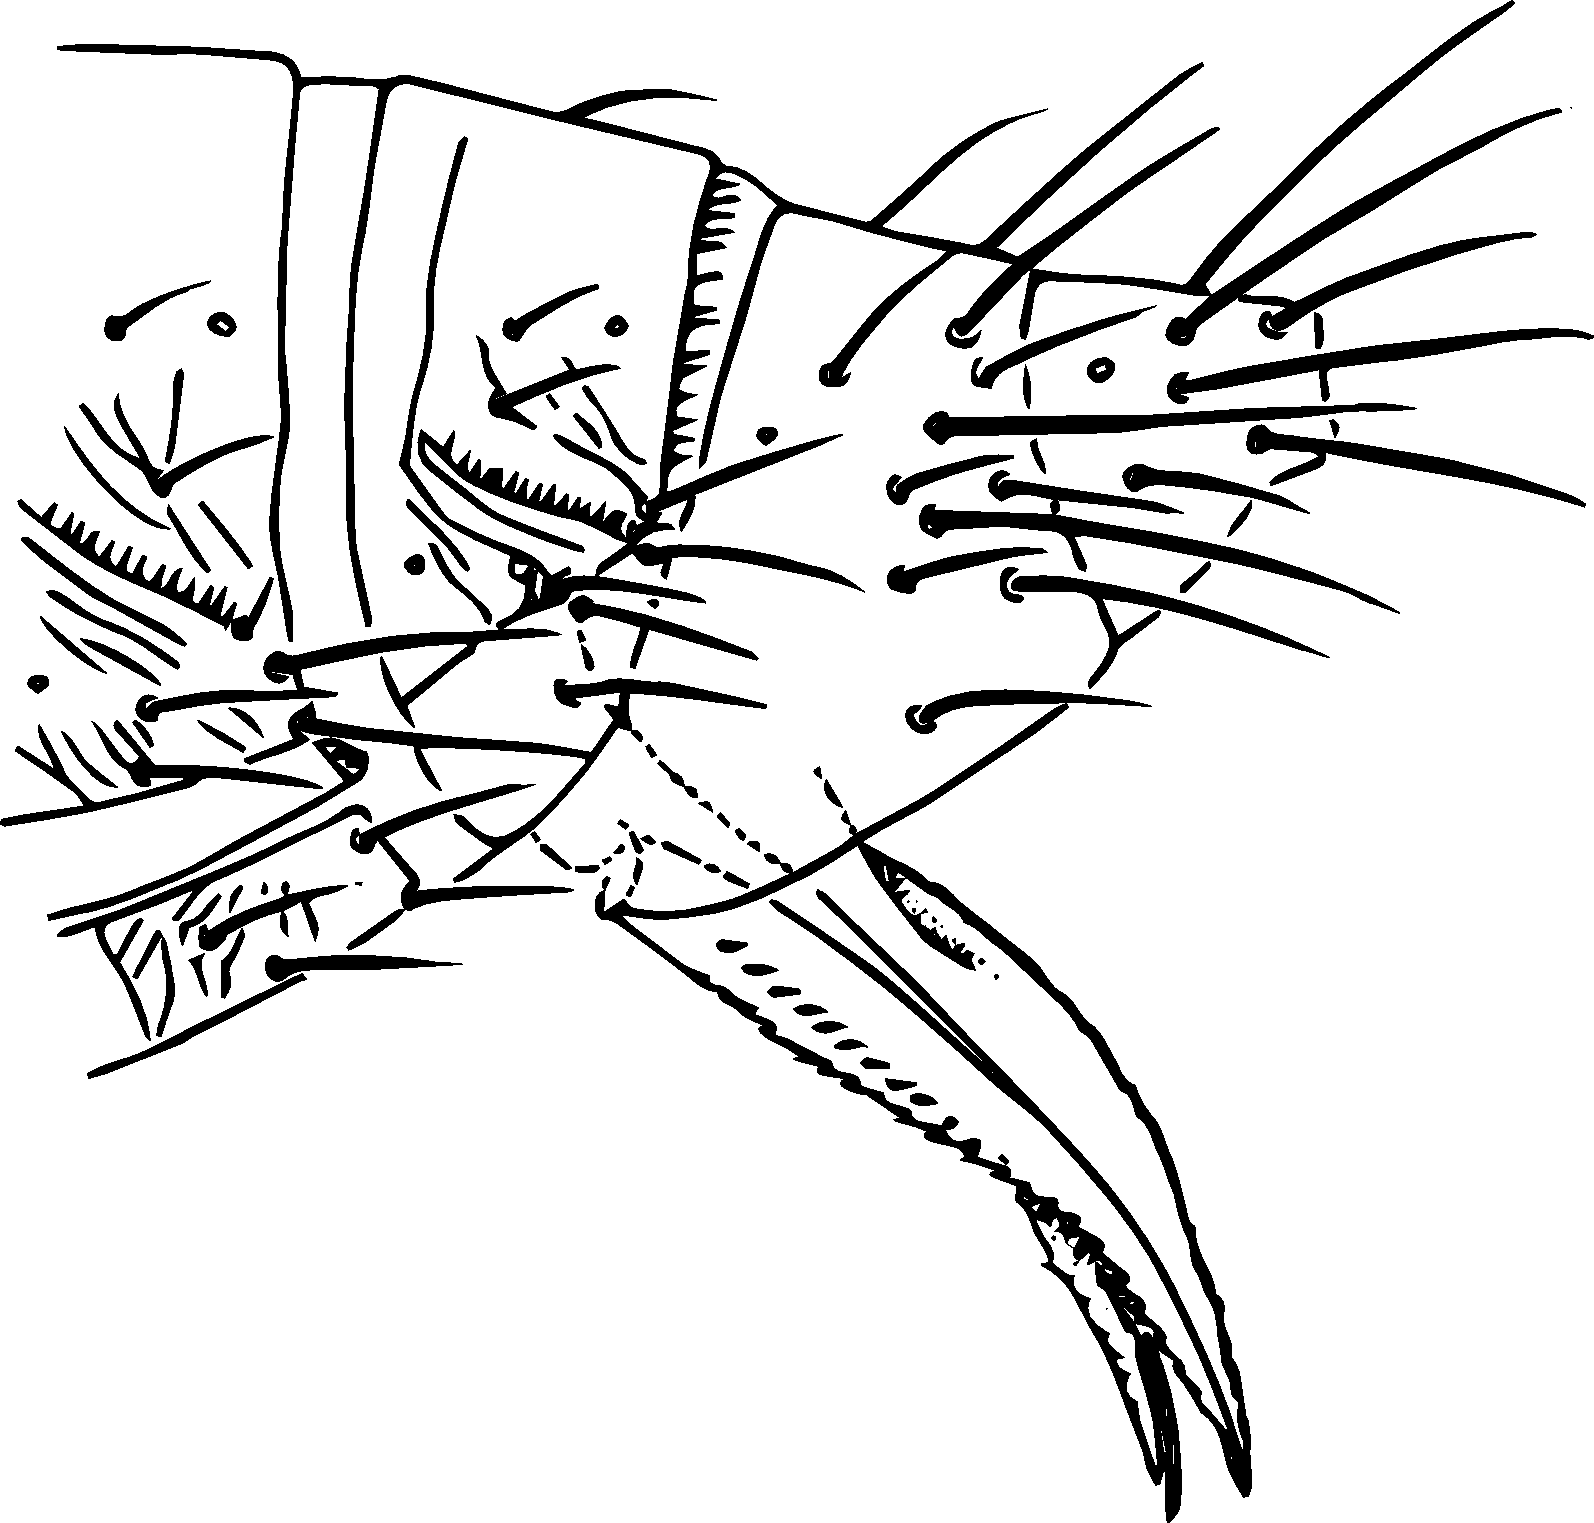
\includegraphics[width=\textwidth]{sections/img/acercaria/TerebrantiaOvipositor.pdf}
  \caption{}
  \label{fig:thripid2}
 \end{subfigure}
 \caption{Thripidae. \textbf{(a)} Dorsal habitus \citep[][Fig. 150]{bhlitem38199}; \textbf{(b)} lateral view of abdomen apex and ovipositor (modified from figure by Annette K. Walker, Manaaki Whenua / Landcare Research, New Zealand}\label{fig:thripid}
\end{figure}

\subsection{Tubulifera}\index{Tubulifera}
\subsubsection{Phlaeothripidae (tube-tailed thrips)}\index{Phlaeothripidae}
\noindent{}\textit{Diagnostic characters:} terminal abdominal segment tubular, not divided; ventrally, with parallel lateral margins (figure \ref{fig:phlaeothripid2}); ovipositor absent; wings with short, bare longitudinal veins and no acanthae (figure \ref{fig:phlaeothripid2}).\vspace{3mm}

\noindent{}\textit{Natural history:} Approximately 3,000 species have been described worldwide. This family includes many species that gallers, and many of them are eusocial. Other species survive as fungivores or herbivores.

\begin{figure}[ht!]
 \centering
 \begin{subfigure}[ht!]{0.48\textwidth}
  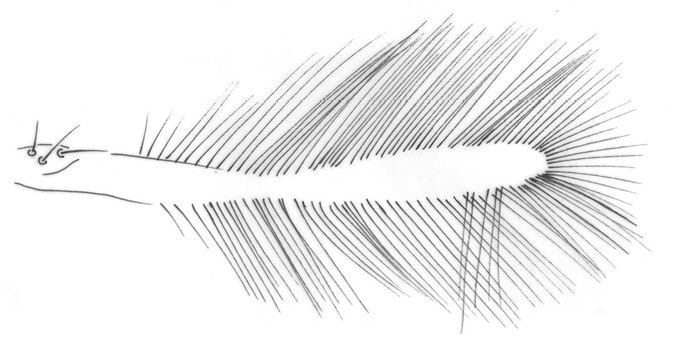
\includegraphics[width=\textwidth]{acercaria/PhlaeothripidWing}
  \caption{}
  \label{fig:phlaeothripid1}
 \end{subfigure}
 \qquad
 \begin{subfigure}[ht!]{0.34\textwidth}
  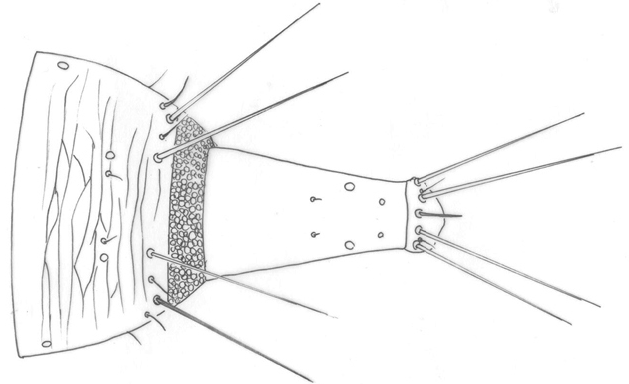
\includegraphics[width=\textwidth]{acercaria/PhlaeothripidAbdomen}
  \caption{}
  \label{fig:phlaeothripid2}
 \end{subfigure}
 \caption{Phlaeothripidae. \textbf{(a)} Fore wing \citep[][Fig. 6]{minaei2013}; \textbf{(b)} dorsal view of abdomen apex \citep[][Fig. 9]{minaei2013}}\label{fig:phlaeothripids}
\end{figure}

\section*{Test yourself}
What traits exhibited by this lineage (Acercaria) might explain the multiple independent origins of hematophagy? Ancestral acercarians possibly fed on fungi; what did the transitions to feeding on blood look like? Why are no Sternorrhyncha parasitic on animals?\vspace{3mm}

\noindent{}There remains some \sout{question} fading speculation regarding the monophyly of Acercaria. Think about the putative synapomorphies listed at the start of this section and the traits you observed in lab. Do you think these three orders are the only ones to evolve from a single common ancestor? If so, what did that ancestor look like?

\clearpage
\thispagestyle{empty}
